\documentclass[11pt,letterpaper]{article}

%%%%%%%%%%%%%%%%%%%%%%%%%%%%%%%%%%%%%%%%%%%%%%%%%%%%%%%%%%%%%%%%%%%%%%%%%
\pagestyle{plain}                                                      %%
%%%%%%%%%% EXACT 1in MARGINS %%%%%%%                                   %%
\setlength{\textwidth}{6.5in}     %%                                   %%
\setlength{\oddsidemargin}{0in}   %% (It is recommended that you       %%
\setlength{\evensidemargin}{0in}  %%  not change these parameters,     %%
\setlength{\textheight}{8.5in}    %%  at the risk of having your       %%
\setlength{\topmargin}{0in}       %%  proposal dismissed on the basis  %%
\setlength{\headheight}{0in}      %%  of incorrect formatting!!!)      %%
\setlength{\headsep}{0in}         %%                                   %%
\setlength{\footskip}{.5in}       %%                                   %%
%%%%%%%%%%%%%%%%%%%%%%%%%%%%%%%%%%%%                                   %%
\newcommand{\required}[1]{\section*{\hfil #1\hfil}}                    %%
\renewcommand{\refname}{\hfil References Cited\hfil}                   %%
\bibliographystyle{unsrt}                                              %%
%%%%%%%%%%%%%%%%%%%%%%%%%%%%%%%%%%%%%%%%%%%%%%%%%%%%%%%%%%%%%%%%%%%%%%%%%
%\usepackage[square, comma, sort&compress]{natbib}

\usepackage[font=small,format=plain,labelfont=bf,up,textfont=it,up]{caption}
\def\abovecaptionskip{1mm} 
\usepackage[margin=1in]{geometry}
\usepackage{url}
\usepackage{alltt}

\usepackage{cite}
\usepackage{bigstrut}
\usepackage{textcomp}
\usepackage{multirow}
\usepackage{rotating}
\usepackage{subfigure}
\usepackage{wrapfig}
\usepackage{hhline}
\usepackage{epsf}
\usepackage{nameref}
\usepackage{enumerate}
\usepackage{amsmath}
\usepackage{subfigure}
\usepackage{wrapfig}
\usepackage{times}
\usepackage{tabularx}
\usepackage{ifthen}
\usepackage{xspace}
\usepackage[usenames]{color}
\usepackage{colortbl}
\usepackage{tabularx}
\usepackage{wasysym}
\usepackage{pdfpages}
\def\naive{na\"{\i}ve}
\def\Naive{Na\"{\i}ve}
\def\naively{na\"{\i}vely}	% Okay, I know, this isn't French.
\def\Naively{Na\"{\i}vely}
\usepackage[compact]{titlesec}
\usepackage[T1]{fontenc}
\usepackage[latin1]{inputenc}
\usepackage[table]{xcolor}
\newcommand{\TODO}[1]{{\it \color{blue}\{TODO: #1\}}}

\usepackage{titlesec}

\urlstyle{same}

%list margin
\usepackage{enumitem}
\usepackage{makecell}

\graphicspath{{figures/}}
\DeclareGraphicsExtensions{.pdf, .png, .ps}

\newboolean{hidecomments}
\setboolean{hidecomments}{true}
\ifthenelse{\boolean{hidecomments}}
{\newcommand{\nb}[2]{}}
{\newcommand{\nb}[2]{
    \fbox{\bfseries\sffamily\scriptsize#1}
    {\sf\small$\blacktriangleright$
      {#2} $\blacktriangleleft$}}}
    
\newcommand\emh[1]{\nb{EMH}{#1}}
\newcommand\myTitle{\newpage
\begin{center}
{\bf SHF:Small: Mega-Transfer: Learning from 10,000+ Software Projects}\\
Tim Menzies (North Carolina State University)
\end{center}}

\usepackage{tikz}
%\newcommand*\circled[1]{\tikz[baseline=(char.base)]{
 %           \node[shape=circle,fille=.,draw,inner sep=2pt] (char) {\color{-.} \bfseries\footnotesize#1};}}

\definecolor{Gray}{gray}{0.9}
\definecolor{darkgray}{gray}{0.8}
\newcommand{\circled}[1]{\tikz[baseline=(myanchor.base)] \node[circle,fill=darkgray,inner sep=1pt] (myanchor) {\color{.}\footnotesize \textbf{#1}};}

\usepackage{bbding}
\definecolor{lgray}{gray}{0.9}

\usepackage{enumitem}
\setlist{nosep}
\usepackage{todonotes}

\newcommand{\bi}{\begin{itemize}}
\newcommand{\ei}{\end{itemize}}
\newcommand{\be}{\begin{enumerate}}
\newcommand{\ee}{\end{enumerate}}

\newcommand{\tion}[1]{\S\ref{sec:#1}}
\newcommand{\tab}[1]{Table~\ref{tab:#1}}

\newcommand{\tbl}[1]{Table~\ref{tbl:#1}}
\newcommand{\fig}[1]{Figure~\ref{fig:#1}}
\newcommand{\eq}[1]{Equation~\ref{eq:#1}}

%\newcommand{\THAT}[0]{ISOP}
\newcommand{\THAT}[0]{ISOP}
\newcommand{\THIS}[0]{\mbox{this proposal}}
% paraHead
\newcommand\paraHead[1]{\noindent\textbf{#1}}
\newcommand\head[1]{\paragraph{\underline{#1}}} 
\usepackage{titlesec}


\titlespacing*{\section}
{0pt}{0ex}{0ex}
\titlespacing*{\subsection}
              {0pt}{0pt}{0pt}
\titlespacing{\paragraph}{0pt}{3pt}{1em}
              
\newcommand{\quart}[4]{\begin{picture}(80,4)%1
	{\color{black}\put(#3,2){\circle*{4}}\put(#1,2){\line(1,0){#2}}}\end{picture}}
\usepackage[font=small,format=plain,labelfont=bf,textfont=it]{caption}

\usepackage{xcolor}
\pagenumbering{arabic}
\usepackage{enumitem}
\setlist{nosep}


\pagenumbering{arabic} 

\usepackage{pifont} 

\begin{document}
\pagestyle{plain}
\myTitle
%\pagenumbering{arabic}
\pagestyle{empty}

\head{Overview:}
Software analytics is a workflow that distills large amounts of low-value data into small chunks of very high-value data. 
What are the implications of big data for software analytics? Currently, researchers have ready access to 10,000+ projects. 
Using all that data, can we learn better models for software quality?  Or is learning from so much big data in software engineering inherently so confusing that no general models can be found?
Currently, there are no answers to these questions in the field of software engineering.  The experience in other fields is that the
{\em more} training data,  the {\em better} the learned model. This effect has yet to be seen in software engineering,
but that might just mean we have yet to use enough training data (hence, this proposal).

In this research, we will test for   better software analytics
via ``mega-transfer''; i.e. searching  10,000+ software projects for lessons learned that are relevant to particular projects.
Mega-transfer will  be tested on 10,000+  of software projects monitored inside public code repositories (e.g. Github) and commercial cloud platform 
like those run in  the Raleigh Research Triangle,  North Carolina.  
That cloud-based DevOps tool build, runs, and deploys, code written in Java, Node.js, Go, PHP, Swift, Python, Ruby Sinatra,Ruby on Rails (and is extensible to other languages). It is is used regularly by 100,000+ developers working on 1600 live projects.


The research  will ask and answer the question:
\begin{center}
{\em Can mega-transfer learning  between 10,000+ project generate better, more insightful, models?}
\end{center}
 
In order to demonstrate the external validity of our methods, we will watch for new releases of the projects we are studying. When such new releases occur, we will apply our current models to those new releases. This will demonstrate the value (or otherwise) of our models on new data.


\head{Intellectual Merit:} 
  In this era of big data, it is timely to ask ``when is enough data, enough?''.
Within all the current industrial focus on industrial big data methods, there is very
little discussion on the value (or otherwise) of using all the available data.
Given the diversity of software projects, accessing more data means accessing data from a diverse range of different projects. 
That is, there might be limits to the big data advantage in SE since,  as we look at more and more data, we are not sampling more items from the {\em same } population. This might mean that software analytics needs to set limits on how much data it uses to make conclusions.


More generally, we ask are there general models of SE that apply to a wide range of projects? Or should all projects be treated as unique entities
that require unique treatments? Note that the latter conclusion would imply a limit to theory development in software engineering.
 

\head{Broader Impacts:}
This proposal focuses on issues of
tremendous economic importance--  the creation of better quality software.
As a result, this work will increase America's ability for industrial and academic innovators to conduct
more scientific studies via computational means.  
 

 The PI teaches senior-level and graduate-level SE, and data mining classes (and in those data mining classes, all the case studies come from software engineering).  All of the technology developed in this proposal will become case study material for those subjects.   The PI will continue his established tradition of graduating  research  students  for  historically  under-represented  groups.   Also, this work will inform the curriculum of the PI's annual
   NSF-funded REU (research experience for undergraduates) work on  the ``Science of Software''
   (in  this program, places are reserved for students from traditionally under-represented areas; e.g.  economically challenged regions of the state of North Carolina) and/or students from universities lacking advanced research facilities). While some of the concepts of this grant would be too advanced for that group, some of the simpler data mining concepts would be suitable for lectures and REU projects.


\head{Keywords:} software analytics, transfer learning,  prediction
\newpage
\pagestyle{plain}

\setcounter{page}{1}
\renewcommand{\thepage} {D--\arabic{page}}
\myTitle

\head{1. OVERVIEW:} 
% In 2013-2014, eleven million programmers \cite{abel14} and half a trillion dollars \cite{gartner14} were spent on information technology. Such a large and growing effort should be managed and optimized via well-researched conclusions. To assist in achieving this, there has been a growing recognition within the software engineering research community of the importance of systematic knowledge collection~\cite{paivarinta15},~\cite{sjoberg08},~\cite{stol2015theory}. Knowledge-building needs to be an iterative process, in which results from practice are used to refine knowledge, then that knowledge is  used to inform future observation and data collection \cite{paivarinta15},~\cite{stol2015theory}. It is no coincidence that it is standard practice in other fields, such as medicine, to continually revisit old conclusions in the light of new theories \cite{prasad13}.
Software analytics distills large amounts of low-value data
into small chunks of very high-value data. For example, after examining many software projects,
it might be concluded that certain coding styles are more bug prone and, hence, should
be depreciated.
A challenging problem with     analytics is the pace of change
in   software. Numerous results~\cite{Pa11,Jo09,De16,Me17} report   many prior beliefs
about software engineering (SE) must now be revised due to the ever-changing nature of the tools,
techniques, and practices.
The hypothesis to be tested in this work is that we can create and maintain
 better  up-to-date quality policies for software projects using  {\bf human-augmented data miners}. Participants at a recent
 Dagstuhl meeting on software analytics~\cite{gall_et_al14}  agreed that human insight can, sometimes, add much value to an automatically 
 learned models. For example,  Shull et al.~\cite{shull02} and Kocaguneli et al.~\cite{kocaguneli2013distributed} both report cases where human insight was critical to avoiding ridiculous errors in software analytics. Further, those insights were central to the creation of the final models (generated
 as part of that work).

But how to collect those insights in a manner that scales to include a very large number of projects?  Consider, for example, the cloud
programming IDE developed 
by our industrial partners here at the Raleigh Research Triangle, North Carolina. 
This platform is an integrated DevOps tool that  build, run, deploy, and  manage  applications written in   Java, Node.js,  Go, PHP,  Swift,  Python,  Ruby  Sinatra,  Ruby  on Rails (and could  easily extended to support other languages  such  as  Scala).   At  the  time of this writing, this platform is used regularly by 1.6 million developers working on   1600 live projects on a variety of software analytics dashboards\footnote{There are  538 proprietary projects, plus over 1100 repositories marked as ``most trending'' at Github.}.  This cloud platform collects the {\em internal attributes} of \tab{metrics} which means, in turn,
that our analytics tools can  find answers about the {\em internal quality attributes}
shown in that table.
The  dashboards of this IDE generate thousands of conclusions
per day about all these projects  (later in this proposal, we give specific examples of those conclusions).

 In theory, given all the developers   reflecting on all those conclusions,  it should be possible to obtain useful feedback from
 a very large number of projects. 
 To test if this is so,  we propose  an innovative  method that debates  different ideas about software quality. {\em Particle swarm optimization} (PSO)~\cite{banks2008review,banks2007review}  is used to implement an arena in which novel extensions to old ideas must
compete to demonstrate their value (ideas without merit are ignored).  
This approach  will be tested on    tasks
such as (a)~predicting the time required to close issues; 
(b)~predicting  how many developers should be assigned to a software task;
(c)~predictors for the locations of bug in software;
(d)~ planners for recommending methods to change all the above (which would be used if managers do not like the predicted values).
These tasks are all ones that  PI Menzies has previously explored, using automatic data miners~\cite{Me13,krishna16,Kr16,rees2017better,Lu12,agrawal17,Me07,Me17}. Here, we extend that
  work by asking:
 
 \begin{center}
{\em Are human-augmented data miners      
 ``better'' for  software  analytics? }
\end{center}
 (i.e.,  ``better'' than  state of the art quality predictors or planners in the SE literature.)

 



 
One significant feature of this work is its
{\bf immediate industrial applicability}. We assert our research has such applicability  for two reasons.
{\em Firstly},
our methods
will be based around software tools in widespread industrial use (Jira, Github, Travis CI, etc).  We will release all our tools via open source licenses so our
results can be  readily applicable to the many research or development teams using Jira, Github, etc.


{\em Secondly}, we will produce not only predictors but also {\em planners}
for how to change software projects in order to improve quality with  that
 project.
 Why are such planners important? At a recent ASE'15 workshop on 
``Actionable Analytics''~\cite{Krishna15a}, industrial practitioners were very
clear in their protest against complex software analytics that offer no insight on what to do in order to improve their projects.
Much of the current work in software analytics, they said,  is on 
{\em prediction} of ``what is'' rather than {\em planning}  of ``what to do''.
 Accordingly, this proposal focuses particularly on the issue of generating plans describing what to do.
   For a formal description on the difference between  planners and predictors,  see  \tab{planprd}.



% Please add the following required packages to your document preamble:
% \usepackage{multirow}
\begin{table}[!t]
\scriptsize
\centering
\resizebox{.9\linewidth}{!}{
\begin{tabular}{l|ll}
\hline
\textbf{ENTITIES} & \multicolumn{2}{c}{\textbf{ATTRIBUTES}} \\  
\textit{\textbf{Products}} & \multicolumn{1}{c}{\textit{\textbf{Internal}}} & \multicolumn{1}{c}{\textit{\textbf{External}}} \\ \hline
\multirow{2}{*}{Specifications} & \multirow{2}{*}{\begin{tabular}[c]{@{}l@{}}size, reuse, modularity, redundancy, \\ functionality, syntactic correctness, \dots\end{tabular}} & \multirow{2}{*}{comprehensibility, maintainability, \dots} \\
 &  &  \\
\multirow{2}{*}{Designs} & \multirow{2}{*}{\begin{tabular}[c]{@{}l@{}}size, reuse, modularity, coupling, \\ cohesiveness, inheritance, functionality, \dots\end{tabular}} & \multirow{2}{*}{quality, complexity, maintainability, \dots} \\
 &  &  \\
\multirow{2}{*}{Code} & \multirow{2}{*}{\begin{tabular}[c]{@{}l@{}}CK metrics, McCabe metrics, Halstead metrics,  \\ functionality, algorithmic complexity,,control-flow structuredness, \dots\end{tabular}} & \multirow{2}{*}{\begin{tabular}[c]{@{}l@{}}reliability, usability, maintainability, \\ reusability\end{tabular}} \\
 &  &  \\
Test Data & size, coverage level, \dots & quality, reusability, \dots \\
\dots & \dots & \dots \\  
\textit{\textbf{Processes}} &  &  \\ \hline
\multirow{2}{*}{\begin{tabular}[c]{@{}l@{}}Construction\\ specification\end{tabular}} & \multirow{2}{*}{\begin{tabular}[c]{@{}l@{}}time, effort, \#requirement changes, \\ \dots\end{tabular}} & \multirow{2}{*}{quality, cost, stability, \dots} \\
 &  &  \\
\multirow{2}{*}{Detailed design} & \multirow{2}{*}{\begin{tabular}[c]{@{}l@{}}time, effort, number of specification faults\\ found, \dots\end{tabular}} & \multirow{2}{*}{cost, cost-effectiveness, \dots} \\


 &  &  \\
Testing & time, effort, number of coding faults found, \dots & cost, cost-effectiveness, stability, \dots \\
Maintenance & \#bug reports, \#maintenance requests, \#enhancement requests,\ldots & extensibleness\dots\\
            & \#issues open, \#issues closes, \#issue close time  \dots &   maintainability \dots \\
\dots & \dots & \dots \\  
\textit{\textbf{Resources}} &  &  \\ \hline
%Personnel & age, price, \dots & productivity, experience, intelligence, \dots \\
Teams & size, communication level, structuredness, \dots & productivity, quality, \dots \\
Organizations & size, pace of personnel change %ISO Certification, CMM level 
& Maturity, profitability, \dots \\
Software &   size, \dots & usability, reliability, \dots \\
%Hardware & price, speed, memory size, \dots & reliability, \dots \\
%Office & size, temperature, light, \dots & comfort, quality, \dots \\
\dots & \dots & \dots \\ 
\end{tabular}}
\caption{Some of the attributes we can access via mining of Github repositories and their associated tool chains.
Following  Fenton's~\cite{Fe14} guidance,  attributes are divided into product, process, and resource. Also, {\em internal}
metrics can be measured directly and {\em external} ones
represent the indirect external manifestations of the internal ones.  }
\label{tab:metrics}
\end{table}

\begin{wraptable}{r}{3in}
\small
\caption{ ``Planning'' is different to ``prediction''.}\label{tab:planprd}

\begin{tabular}{|p{.95\linewidth}|}\hline



~~~~~~Formally, we distinguish planning from prediction as follows: predictors in software analytics take the form \mbox{$out = f(in)$}
where {\em in} contains many independent features (such as OO static code metrics) and {\em out} contains some measure of
software quality such as how many defects are present. For software analytics, the function $f$ is learned via data mining (from static code attributes for instance).
On the other hand, a quality planner generates a concrete set of actions that can be taken (as precautionary measures) to significantly reduce the likelihood of defects occurring in the future.

~~~~~~Formally,   consider a software artifact $Z$ (e.g. a code module). Planners
proposes a plan $\Delta$ to adjust attribute $Z_j$ as follows:

{\scriptsize \begin{equation*}
\forall \delta_j \in \Delta :  Z_j =  
\begin{cases}
     Z_j + \delta_j& \text{if $Z_j$ is numeric}\bigstrut[t]\\
    \delta_j              & \text{otherwise}
\end{cases}
\end{equation*}}

With a planner, to (say) simplify a large bug-prone method, our planners
might suggest to a developer to reduce its size (i.e. refactor that
code by, say, splitting it across two simpler functions).
For an example of software that produces plans, see the discussion of
our CrossTREE algorithm~\cite{krishna2017learning,Kr16}, described later in this paper.\\\hline
\end{tabular}
\end{wraptable}


\head{2. MOTIVATION:  Why  New Tools?} 

~\\
 
Before beginning, we digress to ask a basic question:
why do we need new tools to discover insights about software projects? In this age of big data and  hyper-internet connectivity, is it not enough to just:
\bi
\item
Run a few data miners?
\item
Or just ask someone; e.g. post a query to the on-line programmer forum  stackoverflow.com? 
\ei
Clearly, sometimes, there is  benefit in  knowledge found
via automatic methods~\cite{Zimmermann2004}  or social qualitative methods~\cite{seaman1999qualitative}.
However, neither approach is    foolproof. 
Basili and Shull~\cite{shull02} warn that any automatic analysis of project data cannot access  tacit contextual
knowledge known to humans, but not represented in any data set.
 
\begin{figure}[t!]
    \centering
    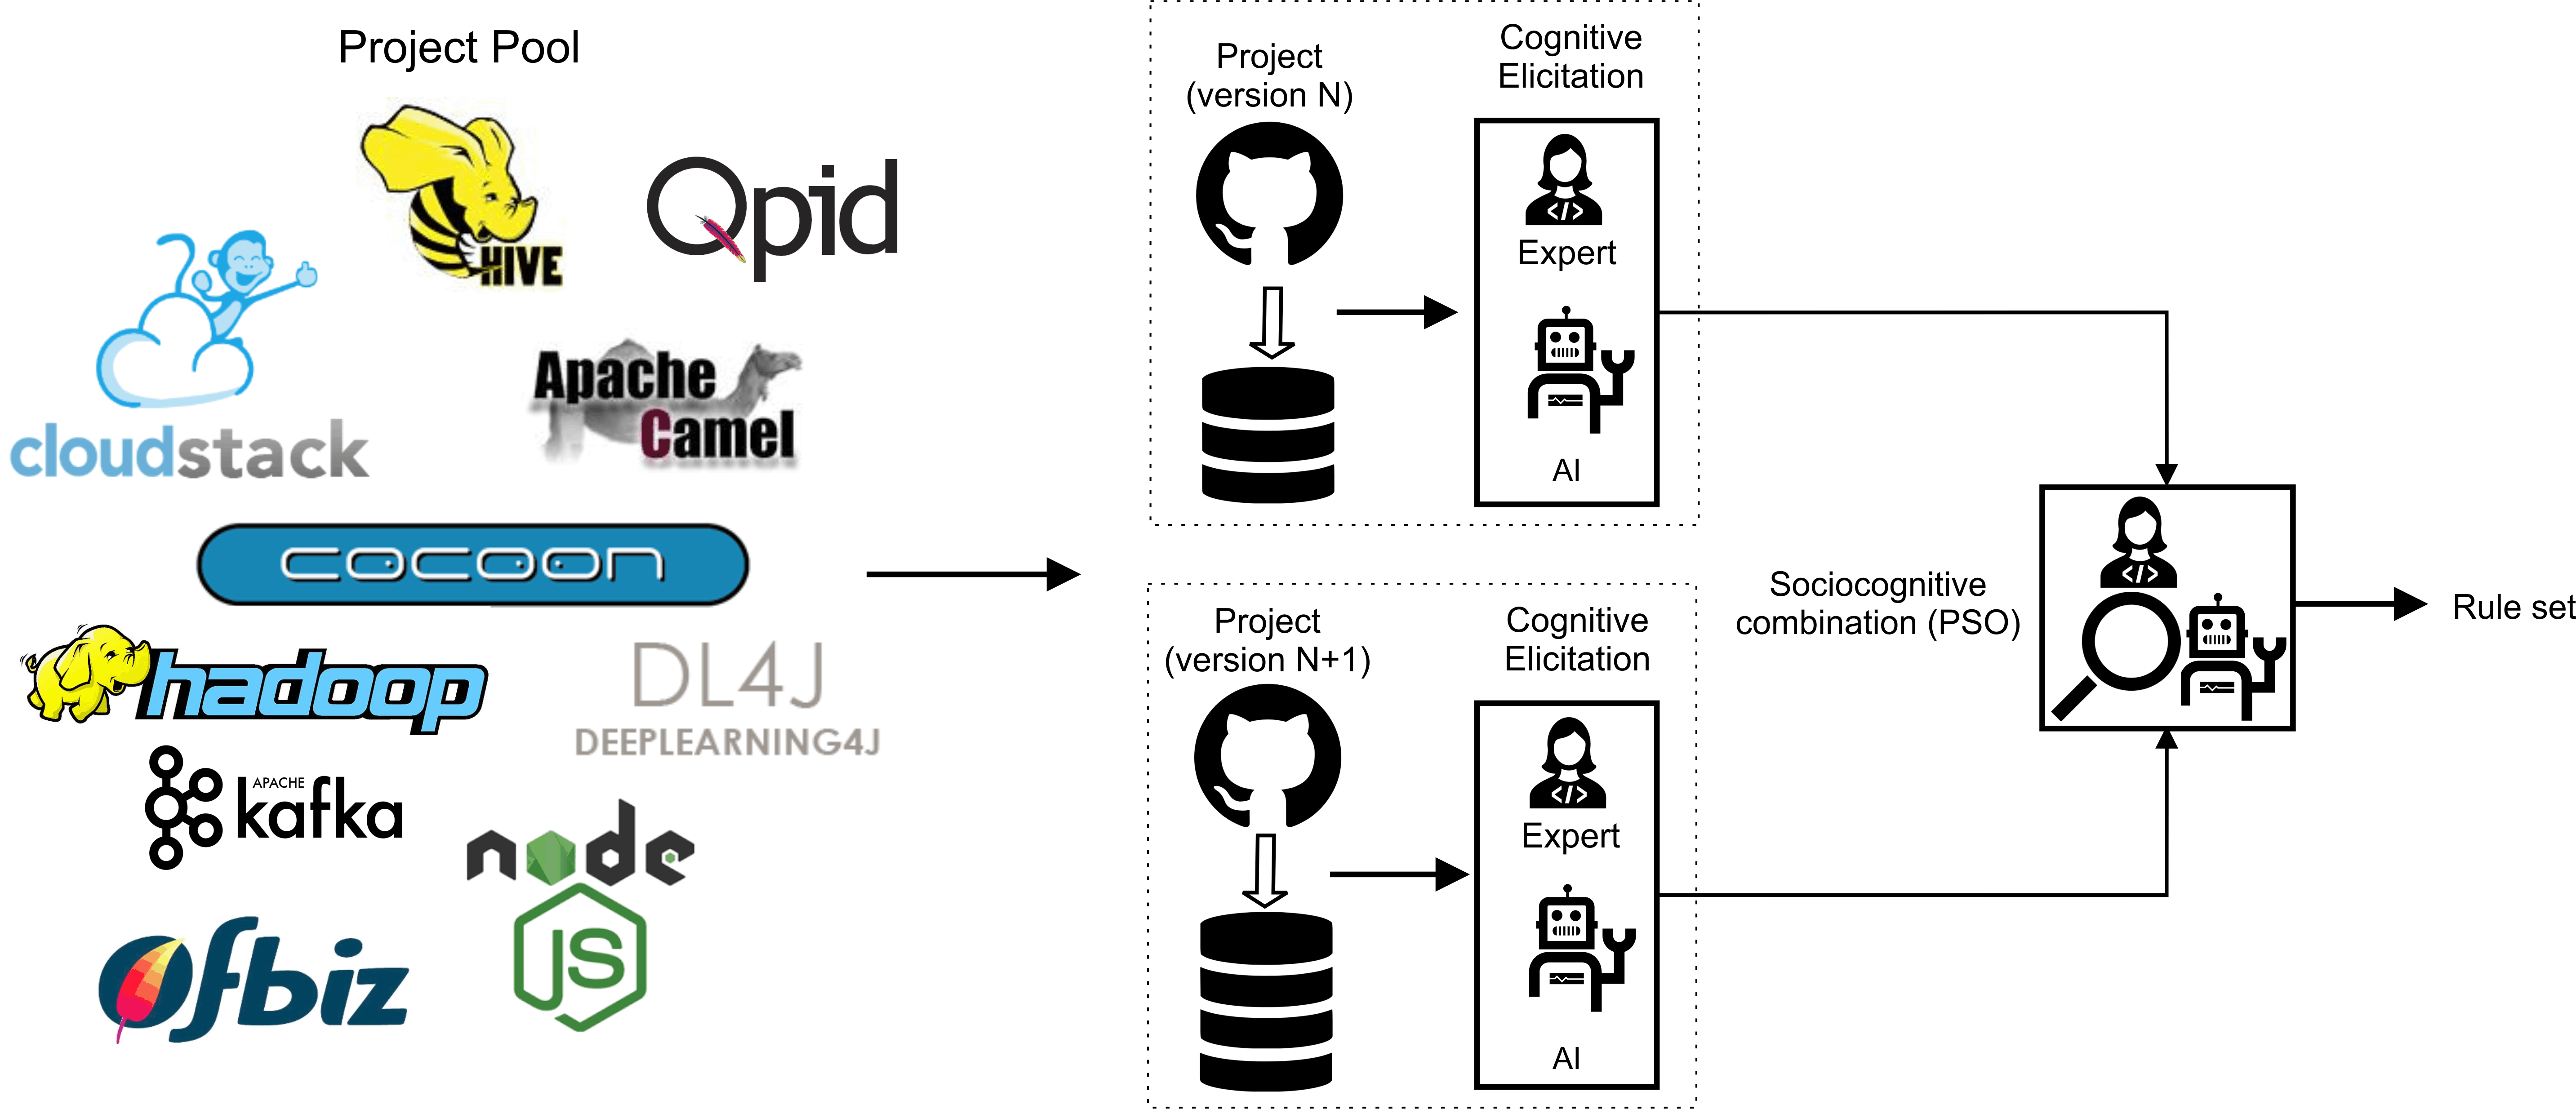
\includegraphics[width=\linewidth]{figs/flow.png}
    \caption{Flowchart of the proposed approach. Humans and AIs comment on data 
    from many projects. This knowledge enters an arena where competing ideas fight it out
    to conclude which are most useful. In this proposal, that arena will be implemented by particle swarm optimization.}
    \label{fig:flow}
\end{figure}

As to eschewing data miners and just using supposed   expert opinion of
developers, that  too  is  problematic.
 Passos et al.~\cite{Pa11} warns that software developers often inappropriately assume whatever worked/failed on their first few projects will also work/fail on all their future projects. They comment  that ``past experiences were taken into account without much consideration for their context''~\cite{Pa11}. 
Other  results by J\o rgensen \& Gruschke~\cite{Jo09} endorse the pessimism of Passos et al. In an empirical study of expert effort estimation, they report that the experts rarely use knowledge patterns from past projects to improve their future reasoning.  
Yet other results have found numerous examples where developers hang on to old ideas, despite evidence to the contrary.
Krishna et al.~\cite{Me17,Kr16}    have conducted   surveys of developers that
  reveal widespread misconceptions and inconsistencies
about the impact of delaying issue resolution in software systems;
and the value (or otherwise) of fixing different kinds of code bad smells.
In a more extensive study of programmers, Devanbu et al.~\cite{De16} surveyed 564 Microsoft software developers from around the world. They found that ``(a) programmers do indeed have very strong beliefs on certain topics; but (b) those beliefs can vary across the personnel within one project, and these usually do not necessarily correspond with actual evidence in that project.'' 

So, what to do? Merely using data miners is not enough since they miss contextual knowledge. And merely
asking developers can lead to misleading results. Perhaps a better way would be to combine human and artificial intelligence.

\head{3. OVERVIEW OF OUR APPROACH: Knowledge Elicitation and Combination} 


In the following, we propose a novel
{\em cognitive} approach that  combines {\em both}   human and artificial intelligence. Our hypothesis, to be tested in this research, is that better analytics 
arise  from {\em combining}
  (a)~an ability to reason over gigabytes of data
 with (b)~data mining with human contextual knowledge. Our approach is in two parts: 
\bi
\item A {\em cognitive elicitation method} that extracts developer insights 
about software. This elicitation method may be designed using data mining or by interacting with domain experts. 
\item A {\em socio-cognitive combination method}  that  combines multiple opinions into one coherent whole using  PSO~\cite{Eb95,banks2008review,banks2007review}. Here,  cognition 
 emerges from the convergence of the beliefs of many individuals. Note that PSO makes no
 assumption that any piece of knowledge is correct. Rather, it is an arena 
 where ideas must  compete to demonstrate their value.
\ei
For readers familiar with the AI literature, we note that alternate methods for combining human and artificial intelligence include Bayesian methods, 
crowdsourcing methods, and 
methods inspired by neuroscience. Those methods are not used here for reasons discussed in our {\em Related Work} section.

% TEXT HERE EXPLAIN FIGURE
The flow chart of the proposed scheme is shown in~\fig{flow}. For every project in the project pool, we mine the repositories and gather the necessary information. Next, we elicit cognitive insights from experts. For reasons discussed in \S2, we also seek to gather insights from tools like CrossTREE following which we combine these rules using a socio-cognitive approach (with PSO).  This approach overcomes a significant drawback with the  CrossTREE system:  CrossTREE has no knowledge on the {\em usability} of its recommendations. Hence, it is prone to produce recommendations that developers can not, or will not, want to change. Our plan is to elicit
feedback from developers to learn which recommendations are feasible (and which aren't).

\fig{venn} visualizes the space of used and ignored recommendations within a software project.
Here \circled{A} shows  all   artifacts that exist in a project and \circled{B} represents the artifacts that can be changed by the developers
of that project. 
Of that set, there is only a subset \circled{C} that developers are actually willing to change.
 \circled{D} is  a subset of the artifacts  that have been changed historically; and
\circled{E} represents the artifacts that CrossTREE recommends fixing. Note that the entire space of possibilities in \circled{A}~--~\circled{E} is not known, nor should we expect to know them. What we do get as the project evolves are a set of points that lie in these sets, i.e., if we watch the projects over time, then the pattern of \fig{venn} should appear. 

\begin{wrapfigure}[10]{l}{0.6\linewidth}
\footnotesize
\centering
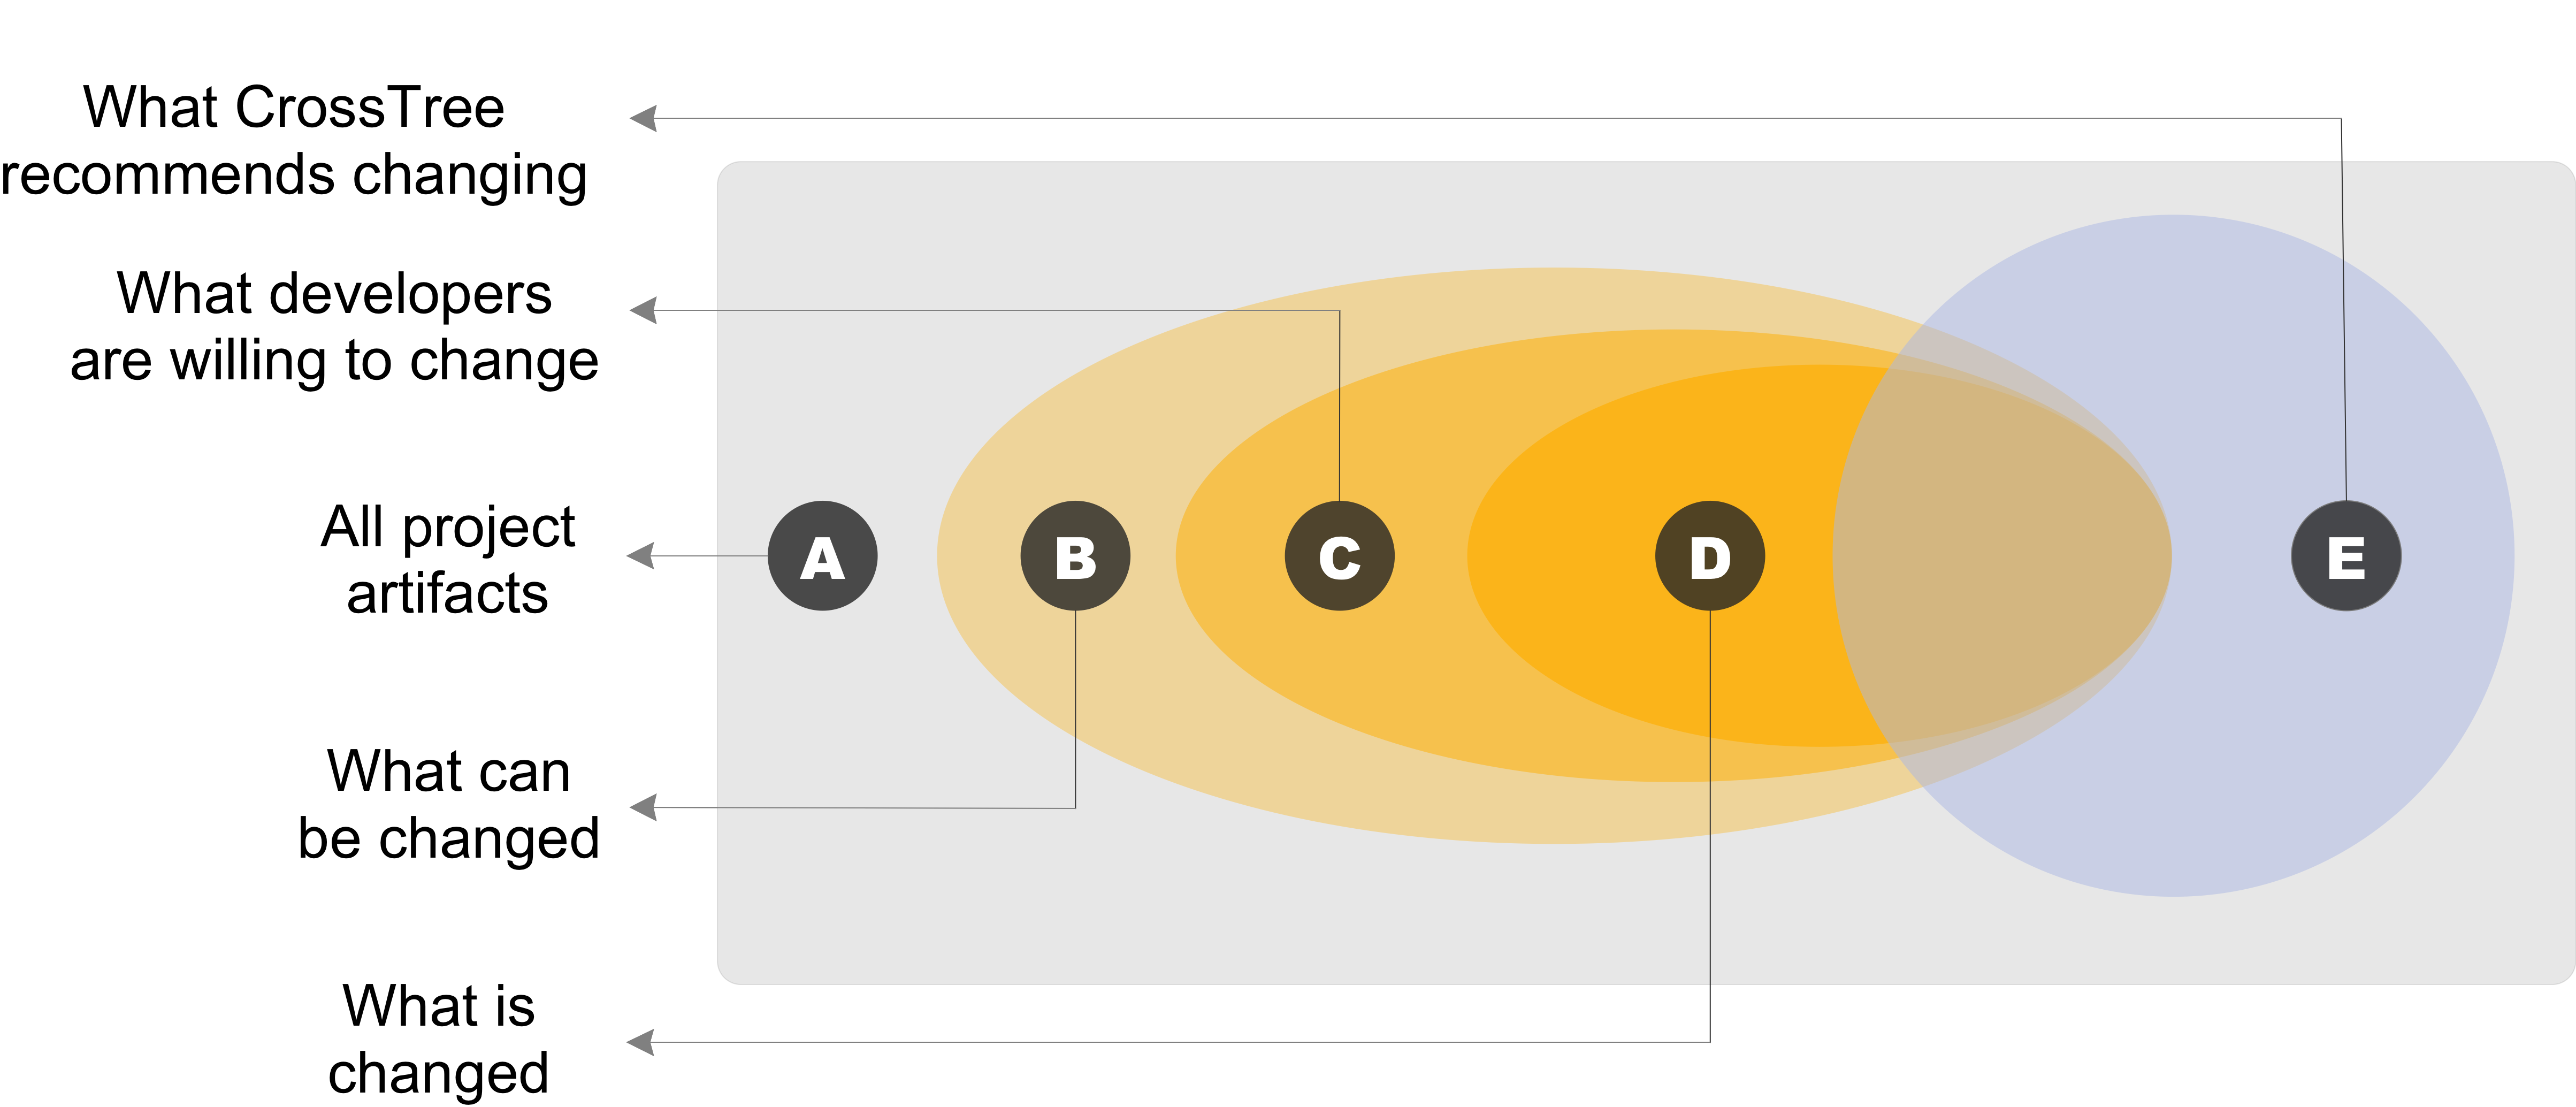
\includegraphics[width=\linewidth]{figs/venn.png}
\caption{Set of possible changes to address project artifacts.}
\label{fig:venn}
\end{wrapfigure} 

Using the sample point in the sets, we would say that developers have the following opinions about CrossTREE's recommendations:
\bi
\item {\em E=Endorsed} = $\circled{D} \cap \circled{E}$; i.e. the    recommendations   developers will actually use; 
\item {\em I=Irrelevant} =  $\circled{E} - \circled{B}$; i.e.  the recommendations  never used (and CrossTREE should avoid these);
\item {\em O=Other} = $\circled{D}- \circled{E}$; i.e. the  changes that developers made but which CrossTREE did not recommend.
\ei

The aim of this project is to explore the space of artifacts in~\fig{venn} so that the recommendations for improving software quality satisfies the following four goal multi-objective problem:
\bi
\item[1.]  {\em Maximize} $E$: the number of   {\em endorsed} recommendations;
\item[2,3.]  {\em Minimize} $I,O$: the  number of {\em irrelevant} and {\em other} recommendations;
\item[4.]  Maximize the  effectiveness of the recommendation as measured by the   $G$ equation of  \fig{xtree_results}.
\ei
\noindent We hypothesize that a socio-cognitive multi-objective evolutionary algorithm such as particle swarm optimization would be an ideal candidate for this purpose.

As a motivating example, for some project ``$X$'' assume that we have the internal attributes: $commit\_id$, $author$, $total\_loc$, $coupling\_between\_objects$, and $cyclomatic\_complexity$. Here, we have:
\bi
\item $\{\mathit{commit\_id,~author,~total\_loc,~coupling\_between\_objects,~cyclomatic\_complexity}\}\in \circled{A}$. The set of all artifacts, measured by a set
of attributes. Note that not all of these are changeable  so any recommendation to change (e.g.) {\em author} would be inappropriate.
Of these, 
\item $\{\mathit{total\_loc,~coupling\_between\_objects,~cyclomatic\_complexity}\}\in \circled{B}$. The set of all artifacts that can be changed.
\item $\{\mathit{coupling\_between\_objects,~cyclomatic\_complexity}\}\in \circled{C}$. The set of all artifacts that the developers are willing to change.
\item $\{\mathit{coupling\_between\_objects,~cyclomatic\_complexity}\}\in \circled{D}$. The set of artifacts that are changed.
\item And finally, $\{\mathit{commit\_id,~total\_loc,~cyclomatic\_complexity}\}\in \circled{E}$. The set of all artifacts that CrossTREE recommends changing.
\ei

\noindent From this, we can derive the following sets:
\bi
\item  {\em E=Endorsed} = $\circled{D} \cap \circled{E}$; i.e. $\{cyclomatic\_complexity\}\in E$
\item {\em I=Irrelevant} =  $\circled{E} - \circled{B}$; i.e.  $\{commit\_id\}\in I$
\item {\em O=Other} = $\circled{D}- \circled{E}$; i.e. $\{coupling\_between\_objects\}\in O$
\ei

\noindent The rules above would in fact be more concrete, e.g. {\em reduce cyclomatic complexity $<15$}. The developers reading these rules 
would keep track of the complexity of the modules they are developing, and split them into smaller modules whenever the cyclomatic complexity of the module exceeds 15. 

The above is an example of one set of insights. For real world projects, we have several thousand such rules which are constantly generated with new project data\footnote{For a real world example of this, see~\fig{bluemix} on page \pageref{fig:bluemix}}. In those cases, we would deploy a PSO with the objectives of: (1) maximizing $E$, (2-3) minimizing $I, O$, and (4) maximizing the effectiveness. The outcome of the PSO would represent the best subset of rules to be applied to a specific case.

\head{4. DETAILS}
This section motivates  our {\em elicitation} and {\em combination} methods
based on CrossTREE and PSO. These tools are developed using principles of cognitive
psychology,  described below. To summarize, we cannot just ask a large cloud of developers to state their knowledge. Rather, for reasons described below,
we will have to query it out of them. In the following, our ``trick'' will learn the useful sections of \fig{venn}.

\noindent
{\bf 4a On the Nature of Human Expertise: }
Recall from {\bf \S{2}}, the results of  Passos, J\o rgensen \& Gruschke, Krishna, 
Devanbu et al.~\cite{Pa11,Jo09,De16,Me17,Kr16}: human software developers have significant trouble explaining
their expertise.  
This is actually
a  known effect; specifically, even 
when humans are quite expert at some task, they can be   inept in explaining how they performed that task~\cite{Fi80,menzies1987micro,menzies94,Compton1990}.  This effect was first seen in the 1970s when researchers struggled to capture  human knowledge in ``expert systems''.
Those researchers found that experts were usually very slow at explaining their expertise;  and when they did, they would say contradictory or incorrect statements~\cite{Fi80}.  

Cognitive psychology~\cite{La81} offers an explanation for this puzzling behaviour of human expertise-- such expertise is stored in a large library of patterns that has been ``compiled'' in such a way as to support fast access, but not
easy browsing of the underlying knowledge. 
Larkin et al.~\cite{La81} characterize human expertise in terms of two memory structures:
\bi
    \item A very small short term memory, or STM, used as a temporary scratch pad for current observation. The short term  memory may be so small that it can hold only 7,  or even 4, items \cite{Mi56}, \cite{Co01}. Recently,  Ma et al.~\cite{Ma14} used evidence from neuroscience and functional MRIs  to  argue  that STM capacity might be better measured using other factors than ``number of items''. But even they conceded that ``the concept of a limited (STM) has considerable explanatory power for behavioral data''.
    \item A very  large long term memory, or LTM, that stores patterns that trigger  on STM contents, perhaps to rewrite the STM  (thus triggering other rules).   The LTM is heavily  indexed, thus  enabling fast reasoning, but complicating the  explication of  that knowledge.  
These LTM patterns are separate tiny  knowledge fragments
that says ``when you see THIS, do THAT''.
\ei
Experts are experts, says Larkin et al.~\cite{La81} because the patterns in their  LTM
patterns dictate what to do, without needing to pause for reflection. On the other hand, novices perform worse than experts when they fill  up  their STM with many to-do's where they plan to pause and reflect on what to do next.  Since, experts post far fewer to-do's  in their STMs, they complete their tasks faster because (a) they are less encumbered by excessive reflection and (b) there is more space in their STM to reason about new information. 

While first proposed in 1981, this STM/LTM theory  still remains relavant~\cite{Ma14}. This theory can be used to explain both expert competency and incompetencies.
 For example, Wiedenbeck et al.~\cite{Wi96}  studied   novice vs expert program comprehension. Experts can reason better than novices  about code written using recurring basic  patterns (e.g. a for loop that iterates for 1 to 10). However, for
an unfamiliar kind of code segment (e.g. a for loop that counts 10 to 1 in jumps of 2), expert performance degrades. This can be explained via the LTM: experts are experts when the recurring basic patterns match their LTM patterns.  Otherwise, when finding code that is unfamiliar to their LTM patterns, their performance deteriorates.

% Similarly, STM/LTM can explain the findings of  Passos, J\o rgensen \& Gruschke, Krishna, 
% Devanbu et al.~\cite{Pa11,Jo09,De16,Me17,Kr16}. We conjecture that since software development is such a rapidly evolving field, it is unlikely that developers will see exactly the same kind
% of project, twice. Hence, LTM patterns learned on old projects are never challenged with new 
% information. According, a developer's LTM fills up with irrelevancies from old projects, thus explaining the results of 
%  Passos, J\o rgensen \& Gruschke, Krishna, 
% Devanbu et al.


%
\begin{wraptable}{r}{0.45\textwidth}
\footnotesize
\centering
\begin{tabular}{|p{0.95\linewidth}|}
\hline
Tasks to be swapped into short-term memory during verification:
\begin{itemize}[leftmargin=*]
  \item Check   singletons return 1 class not N;
  \item Check   streams close in finally block;  
  \item Check  method signatures throw exceptions  caught in method body;
  \item Check   fields are  initialized in constructor;  
  \item Check types being stored in hashmap;
\end{itemize}\\\hline
\end{tabular}
\caption{ Some expert anti-patterns. From~\cite{Jo17}.}
\label{tab:expert_knowledge}
\end{wraptable}


% Another piece of recent research also endorses the currency of this STM/LTM cognitive theory.   Johnson~\cite{Jo17}  found that expert software developers use  their short term memory in special way.   She reports  that one consistent difference between novice and expert developers is that latter built  a list  of ``anti-patterns'' that suggest specific tests that should be applied during testing  (anti-patterns describe a commonly occurring response to a  recurring problem that generates decidedly negative consequences~\cite{Ko95}). One way to summarize the Johnson result is as follows: experts are experts since they know how (sometimes) stupid they can be. Hence, they guard their own systems against their own stupid mistakes via the judicious selection a small number of verification tasks that they will load into the shorter term memory, when the code is being tested. For examples of this kind of expert knowledge found by Johnson, see ~\tab{expert_knowledge}.


% More generally,  Johnson's results  are an example of what Scaife and Rogers  call  external distributed cognition, or DCog~\cite{SCAIFE1996185}.
% DCog explores goal-based activity and
% emphasizes the ways that cognition is off-loaded into the environment through     technological
% and other means. That is, rather than a ``brain in a vat'' model, where all cognition happens
% only between the ears, DCog   involves the coordination between individuals, artifacts and the environment~\cite{Rogers1994}.  



Informed by the above theory, offer two principles of knowledge elicitation that will guide the rest of this research proposal.
\bi
\item {\em Principle\#1:}
never seek   dense richly-connected models from experts.  LTM theory states that human expert knowledge exists as many small fragments.
Hence,  the goal of knowledge elicitation should be to  increase
the rate of discovery  of such  small knowledge fragments. Subsequently  in this proposal, we will use {\em planning
association rules} to represent those fragments.
\item
{\em Principle\#2:} never ask for knowledge directly. Human expertise is buried away inside heavily indexed LTM patterns. Hence, humans have a hard time articulating
that knowledge. An alternate tactic, used by PI Menzies in the 1980s, is ``knowledge elicitation via irritation".   Human experts  are often much more comfortable critiquing than creating knowledge. Hence, rather than asking experts ``what is?'', he found them much more forthcoming when he showed them some initial ``first pass'' knowledge (which was wrong) and ask them  ``is it this?''.  
Back in the 1980s, one draw back with knowledge elicitation by irritation is that 
this ,  ``first pass''  knowledge must be first generated in order to elicit more knowledge. Now, a better ``first pass'' knowledge generator would be  to use a data miner such as CrossTREE   (described below).
\ei
 


 \begin{figure}[!b]
 \hrule
 
 \begin{minipage}{.59\linewidth}
 \vspace{1mm}
\includegraphics[width=3.5in]{figs/XTREE_samp.eps}
\end{minipage}
\begin{minipage}{.40\linewidth}
\small
CrossTREE's plans 
% from improving quality 
are derived from decision trees or regression trees that predict for some software quality
attribute. 
In this example, the tree uses static code attributes to predict for number of bugs
and the leaf values show the probability
that a code module falling here will be buggy. 

For example,  this decision tree is saying that
the ``current branch'' has a `100\% chance of being buggy.
CrossTREE's  {\em plan} is the {\em delta $\Delta$} between
a test instance's current leaf and a nearby {\em desired} leaf with higher quality.
\end{minipage}

\hrule

\caption{CrossTREE: a tutorial. From~\cite{Kr16}.}\label{fig:tutorial}
\end{figure}

\noindent{\bf 4b.   Knowledge elicitation with CrossTREE:}
This section describes the CrossTREE  knowledge elicitation tool
designed using the above two
principles.
 CrossTREEs is an example of the  planning algorithms described in \tab{planprd}. For an example of how
 this algorithm generates plans, see \fig{tutorial}.
 
In 2017, CrossTREE was  deployed into the cloud-based big data development platform described in our introduction. \fig{bluemix} shows a CrossTREE plan, as it is displayed on the dashboard of
that   platform. The circular bar chart 
of that figure shows lines of code in a software system and the red sections denote regions predicted to be buggy.  The recommendations shown on the screen are CrossTREE's
advice for how a developer can reduce the expected number of bugs in their code.

\begin{figure} 
    \centering
    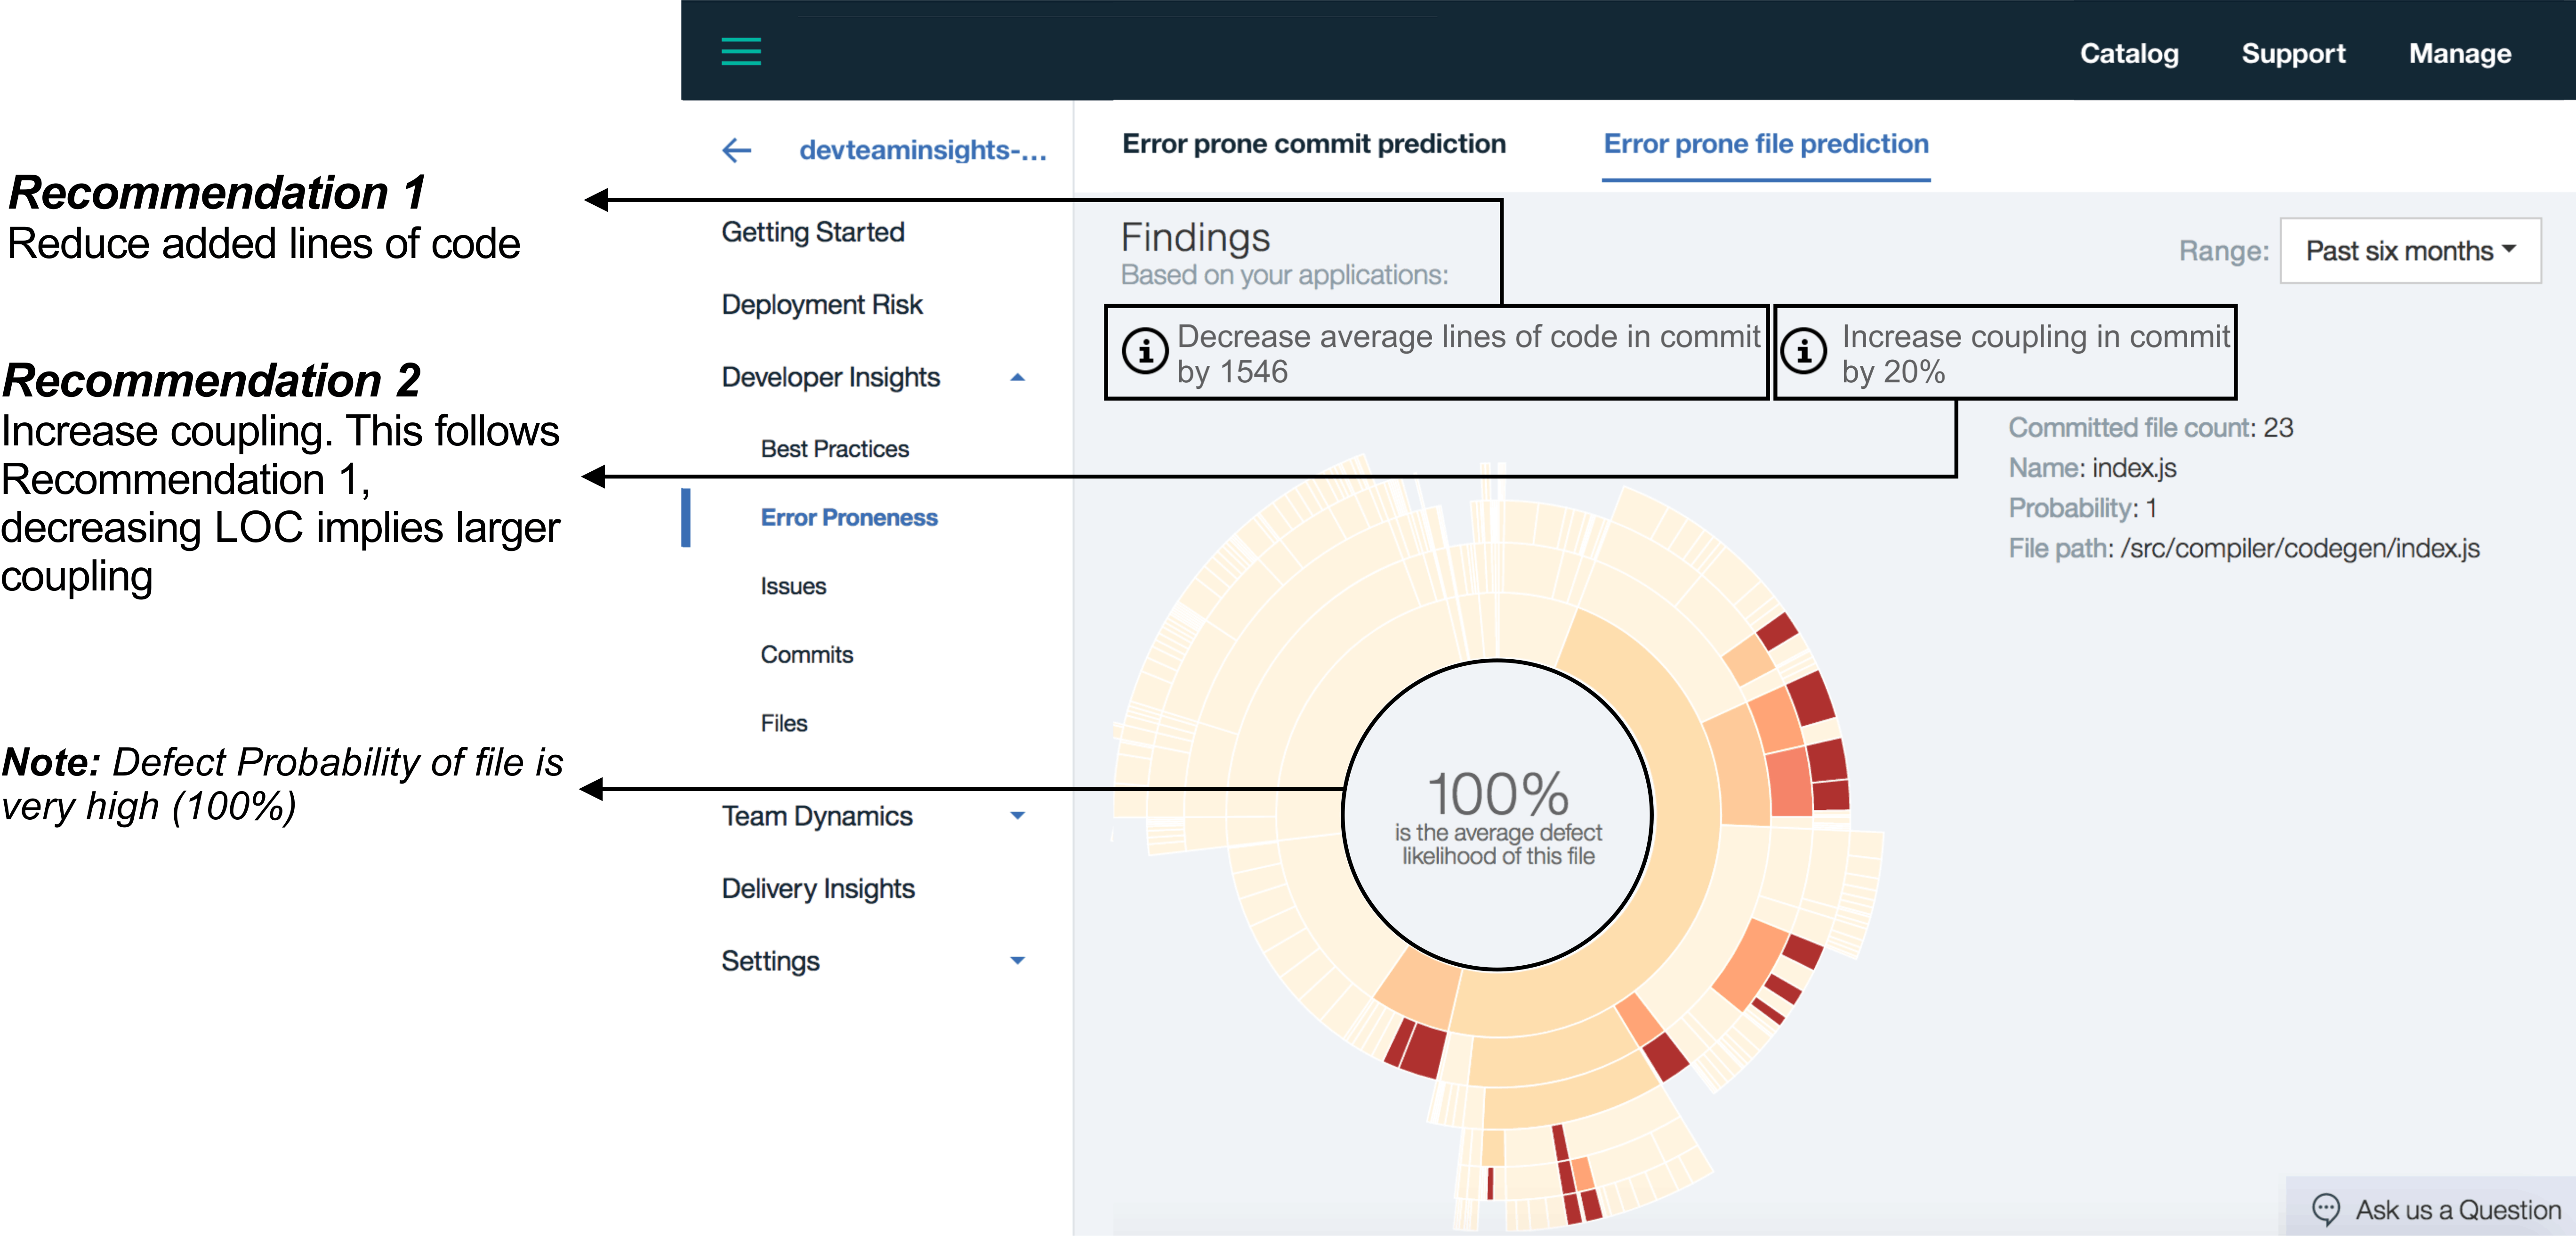
\includegraphics[width=\linewidth]{figs/bluemix.png}
    \caption{The CrossTREEs tools used in this research has already been deployed into
   a cloud-based programmer IDE. The circular display shows lines of ode in a software system
    and the red sections denote regions predicted to be buggy. The recommendations shown on the screen are CrossTREEs' advice
    for how a developer can reduce the expected number of bugs
    in their code. By our reckoning, screens like the above are seen
    by the developers of 1600 projects. Given all that expertise reflecting on our recommendations, the research challenge of this research it so find some way to combine all the insight into better and actionable models of
    software quality
}
    \label{fig:bluemix}
\end{figure}




 \begin{wrapfigure}[11]{r}{3in}
\scriptsize
  
  
 \begin{tabular}{{l@{~~~~}l@{~~~~}|r@{~~~~}r@{}c@{~~~}r}}
\arrayrulecolor{lightgray}
\rowcolor{lightgray}\textbf{Rank} & \textbf{Treatment} & \textbf{Median} & \textbf{IQR~~~} & \\
  1 &         CrossTree &    56   &  21  & \quart{54}{25}{65}{1} \\
\hline  2 &        Alves &    32   &  17  & \quart{28}{20}{37}{1} \\
\hline  3 &     Shatnawi &    15   &  4.2 & \quart{15}{6}{18}{1} \\
\hline \end{tabular}

 
% \textbf{Poi}~~~~~~~~ \begin{tabular}{{l@{~~~~}l@{~~~~}|r@{~~~~}r@{~~}c@{}r}}
% \arrayrulecolor{lightgray}
% \rowcolor{lightgray}\textbf{Rank} & \textbf{Treatment} & \textbf{Median} & \textbf{IQR~~~} & \\
%         1 &         CrossTree &    20   &  16  & \quart{39}{40}{51}{2} \\
% \hline  2 &        Alves &    14   &  16  & \quart{21}{41}{37}{2} \\
%         3 &     Shatnawi &    8   &  1  & \quart{19}{5}{21}{2} \\
% \hline \end{tabular}\\
 
\caption{Somewhat quality
improvement seen in 30 random samples of the data.
measured in terms of $G=100\times(1- v/u)$ (defined in text).
Comparing the effectiveness of CrossTREEs's plans to other methods on two defect data sets.
Median, IQR are 50th   (75-25)th percentiles values.
{\em Larger} values
are {\em better}).
From~\cite{Kr16}.}\label{fig:xtree_results}
\end{wrapfigure}
% {\scriptsize \textbf{Lucene}~ \begin{tabular}{{l@{~~~~}l@{~~~~}|r@{~~~~}r@{~~}c@{}r}}
% \arrayrulecolor{lightgray}
% \rowcolor{lightgray}\textbf{Rank} & \textbf{Treatment} & \textbf{Median} & \textbf{IQR~~~} & \\
%         1 &         CrossTree &    16   &  6  & \quart{50}{29}{71}{4} \\
%         1 &     Shatnawi  &    15   &  2  & \quart{63}{10}{67}{4} \\
% \hline  3 &        Alves  &    9   &  4  & \quart{33}{19}{42}{4} \\
% \hline \end{tabular}}\\
% {\scriptsize \textbf{Ivy}~~~~~~~~ \begin{tabular}{{l@{~~~~}l@{~~~~}|r@{~~~~}r@{~~}c@{}r}}
% \arrayrulecolor{lightgray}
% \rowcolor{lightgray}\textbf{Rank} & \textbf{Treatment} & \textbf{Median} & \textbf{IQR~~~} & \\
%         1 &        Alves &    67   &  20  & \quart{58}{21}{71}{1} \\
% \hline  2 &         CrossTree &    52   &  22  & \quart{42}{24}{55}{1} \\
% \hline  4 &     Shatnawi &    20   &  7  & \quart{18}{8}{21}{1} \\
% \hline \end{tabular}}\\
% {\scriptsize  \textbf{Jedit}~~~~~ \begin{tabular}{{l@{~~~}l@{~~~~}|r@{~~~~}r@{~~}c@{}r}}
% \arrayrulecolor{lightgray}
% \rowcolor{lightgray}\textbf{Rank} & \textbf{Treatment} & \textbf{Median} & \textbf{IQR~~~} & \\
%   1 &        Alves &    36   &  7  & \quart{60}{10}{66}{1} \\
%   1 &        CrossTree &    36   &  0  & \quart{66}{0}{66}{2} \\
%   1 &     Shatnawi &    36   &  9  & \quart{53}{13}{66}{1} \\}
 CrossTREE   is known to generate effective plans  for improving software quality in many   software engineering domains.
With Krishna et al.~\cite{krishna2017learning,krishna16,Kr16}, we have  applied CrossTREE
 plans  to data relating to (a)~predicting issue close time in Github;
(b)~effort estimation; (c)~bad smell detection; and  (d)~defection prediction data. 
In all those domains, Krishna et al.~\cite{krishna2017learning,krishna16,Kr16} showed
 that CrossTREE plans are an effective tool for proposing effective changes to software projects.
 For example, \fig{xtree_results} shows some CrossTREE results for defect prediction.
In this study,
CrossTREE's plans were compared against alternate
plans generated by methods proposed by Alves, Erni, Hermans, Shatnawi et al.~\cite{Al10},~\cite{Er96},~\cite{He15}, and~\cite{Sh10}. These tools were used to assess CrossTREE since they are very  widely cited (as of August 2017, Google Scholar reported that the Alves, Erni, Hermans,and Shatnawi's papers have received  118, 116, 23, and  85 citations, respectively).
All these methods raise an alert if some static code measure crosses some decision boundary;
e.g. Erni et al. raises an alert if any static code measure is above  $\mu+\sigma$  for that static code measure's distribution. 



To compare CrossTREE against these other tools, the following procedure was applied.
First, the available project data was divided into separate {\em train, change} and {\em test} set.
Second, Random Forests were applied to the {\em train} set to learn a verification oracle that can predict the bug-proneness of some section of code.
Random Forests were used since Ghotra and Lessmann et al.~\cite{Gh15},~\cite{Le08} both strongly recommend Random Forest.
Third,  CrossTREE and the other methods were applied to the {\em change} set to generate planners to plan for what to change. For CrossTREE, the planner was generated as per  \fig{tutorial}.
For the other methods, the planners were obtained by adhereing to the thresholds at which these tools raised an alert.
Fourth, we applied the changes recommended in step-3 to the {\em test} set.
Fifth, using the verification oracle built in step-1, we determined how many bugs would be seen if the code was changed as per step~4.
 \fig{xtree_results} shows the resulting performance measures in terms of
   $G=100\times(1- v/u)$ where {\emu u,v} denote the probability of low
quality before, after applying a plan. 
Values near 0
imply no improvement and {\em larger} values are {\em better}.
The $G$ values seen using
CrossTREE's plans are {\em larger},  hence {\em better} that other methods. 
  
  
  Note that   CrossTREE  satisfies   the above    principles of knowledge elicitation discussed in {\bf \S{4a}}:
  \bi
  \item
  \mbox{{\em Principle \#1:}}
CrossTREE's recommendations are not dense richly-connected models. Rather, they read
like LTM fragments; i.e. tiny context-specific knowledge fragments that offer specific advice what to do in specific situations. 
\item
\mbox{{\em Principle \#2:}}, CrossTREE can be used for ``knowledge elicitation via irrigation''.
 Instead of asking developers ``what factors increase software project quality?'' we will
 instead show developers  CrossTREE recommendations, then track what response that evolves. 
Specifically, we will post the recommendation as an issue report. After that,
 it will be clear if developers act
 on that recommendation 
 (i.e. if they accept that issue, then move to close to the issue as ``completed'').
Other researchers~\cite{theisen2017risk} report that such a ``post an issue and see what happens'' tactic is an effective experimentation  for  teams communicate extensively via Github issue reports.  
\ei 

{\bf 4c. Knowledge combination + PSO:} If we believed that there is no value in human insight, then our current
systems, which generates recommendations like \fig{bluemix}, would suffice.  However, our goal is to
test {\em combinations}
of human and artificial intelligence. Therefore, more machinery is required.

This  section describes our PSO architecture.  
We use PSO since it is a  {\em socio-cognitive} approach where
 all inference is made by jostling around
all the  opinions of other members of the community.
This makes it a natural method for exploring a space of possible contradictory opinions, only some of which might   actually be useful
for improving quality.





% Recalling {\bf \S{2}}, our premise is that any assertion from humans or from an AI might  sometimes be wrong.
% Hence, we cannot uncritically accept any such assertion. Instead, we must create an arena 
% where novel extensions to old ideas must compete to demonstrate their value (and ideas that lose that compete will be purged). Note that this arena should always be reviewing old conclusions since, as we saw above
% in \mbox{{\bf \S{2a}}}, one problem
% with SE knowledge is that SE developers fixate on old patterns while rarely revising them.


% Within that arena, we will run a multi-objective optimizers to solve the above  four goal multi-objective problems
% i.e. minimize $(I,O)$ while maximizing $(E,D_i)$.
% To build that arena, we will use the  particle swarm optimization (PSO)~\cite{Eb95} algorithm
% where  particle contains one {\em planning association rule}
%  The details of PSO are discussed below, after some technical notes on planning association rules.
 
 
 Over the past several decades researchers have reported that stochastic algorithms (e.g. PSO, genetic algorithms) can 
 generate very effective rule sets~\cite{Gold85, dejong90, dejon93, vent93,va92}. These stochastic methods have been applied to such diverse domains such as mining rules for credit assignment~\cite{grefen, grefenstette93} and for learning very complex first order logic rules~\cite{Aug95}. Of particular interest to us is the finding that this approach is particularly useful for combining rules derived from expert opinion with machine derived rules~\cite{Ish97}. For
 example, stochastic algorithms can also be extended to synthesize expert opinion with fuzzy control rules~\cite{he98}.
A distinct advantage of generating rules from stochastic algorithms is that it enables discovering a few interesting, high-level prediction rules from the databases, rather than discovering  a large rule set as was the usual practice with other approaches~\cite{Fr98}. Further, using evolutionary algorithms, these rules can also be derived from streaming data without much overhead ~\cite{Vi11}.


For our domains,  rules will take the  form {\em LHS $\rightarrow$ RHS} where $\mathit{LHS} \cap \mathit{RHS}=\emptyset$
 and {\em LHS,RHS} are sets of attribute ranges taken from the project data (we create these ranges using
 the methods described below).
 Each rule is a plan that should be following in a certain context and can be interpreted
 as ``when the LHS is true, change the ranges to the values seen in the RHS''. 
 

 


% \begin{wrapfigure}[15]{R}{0.4\textwidth}
% 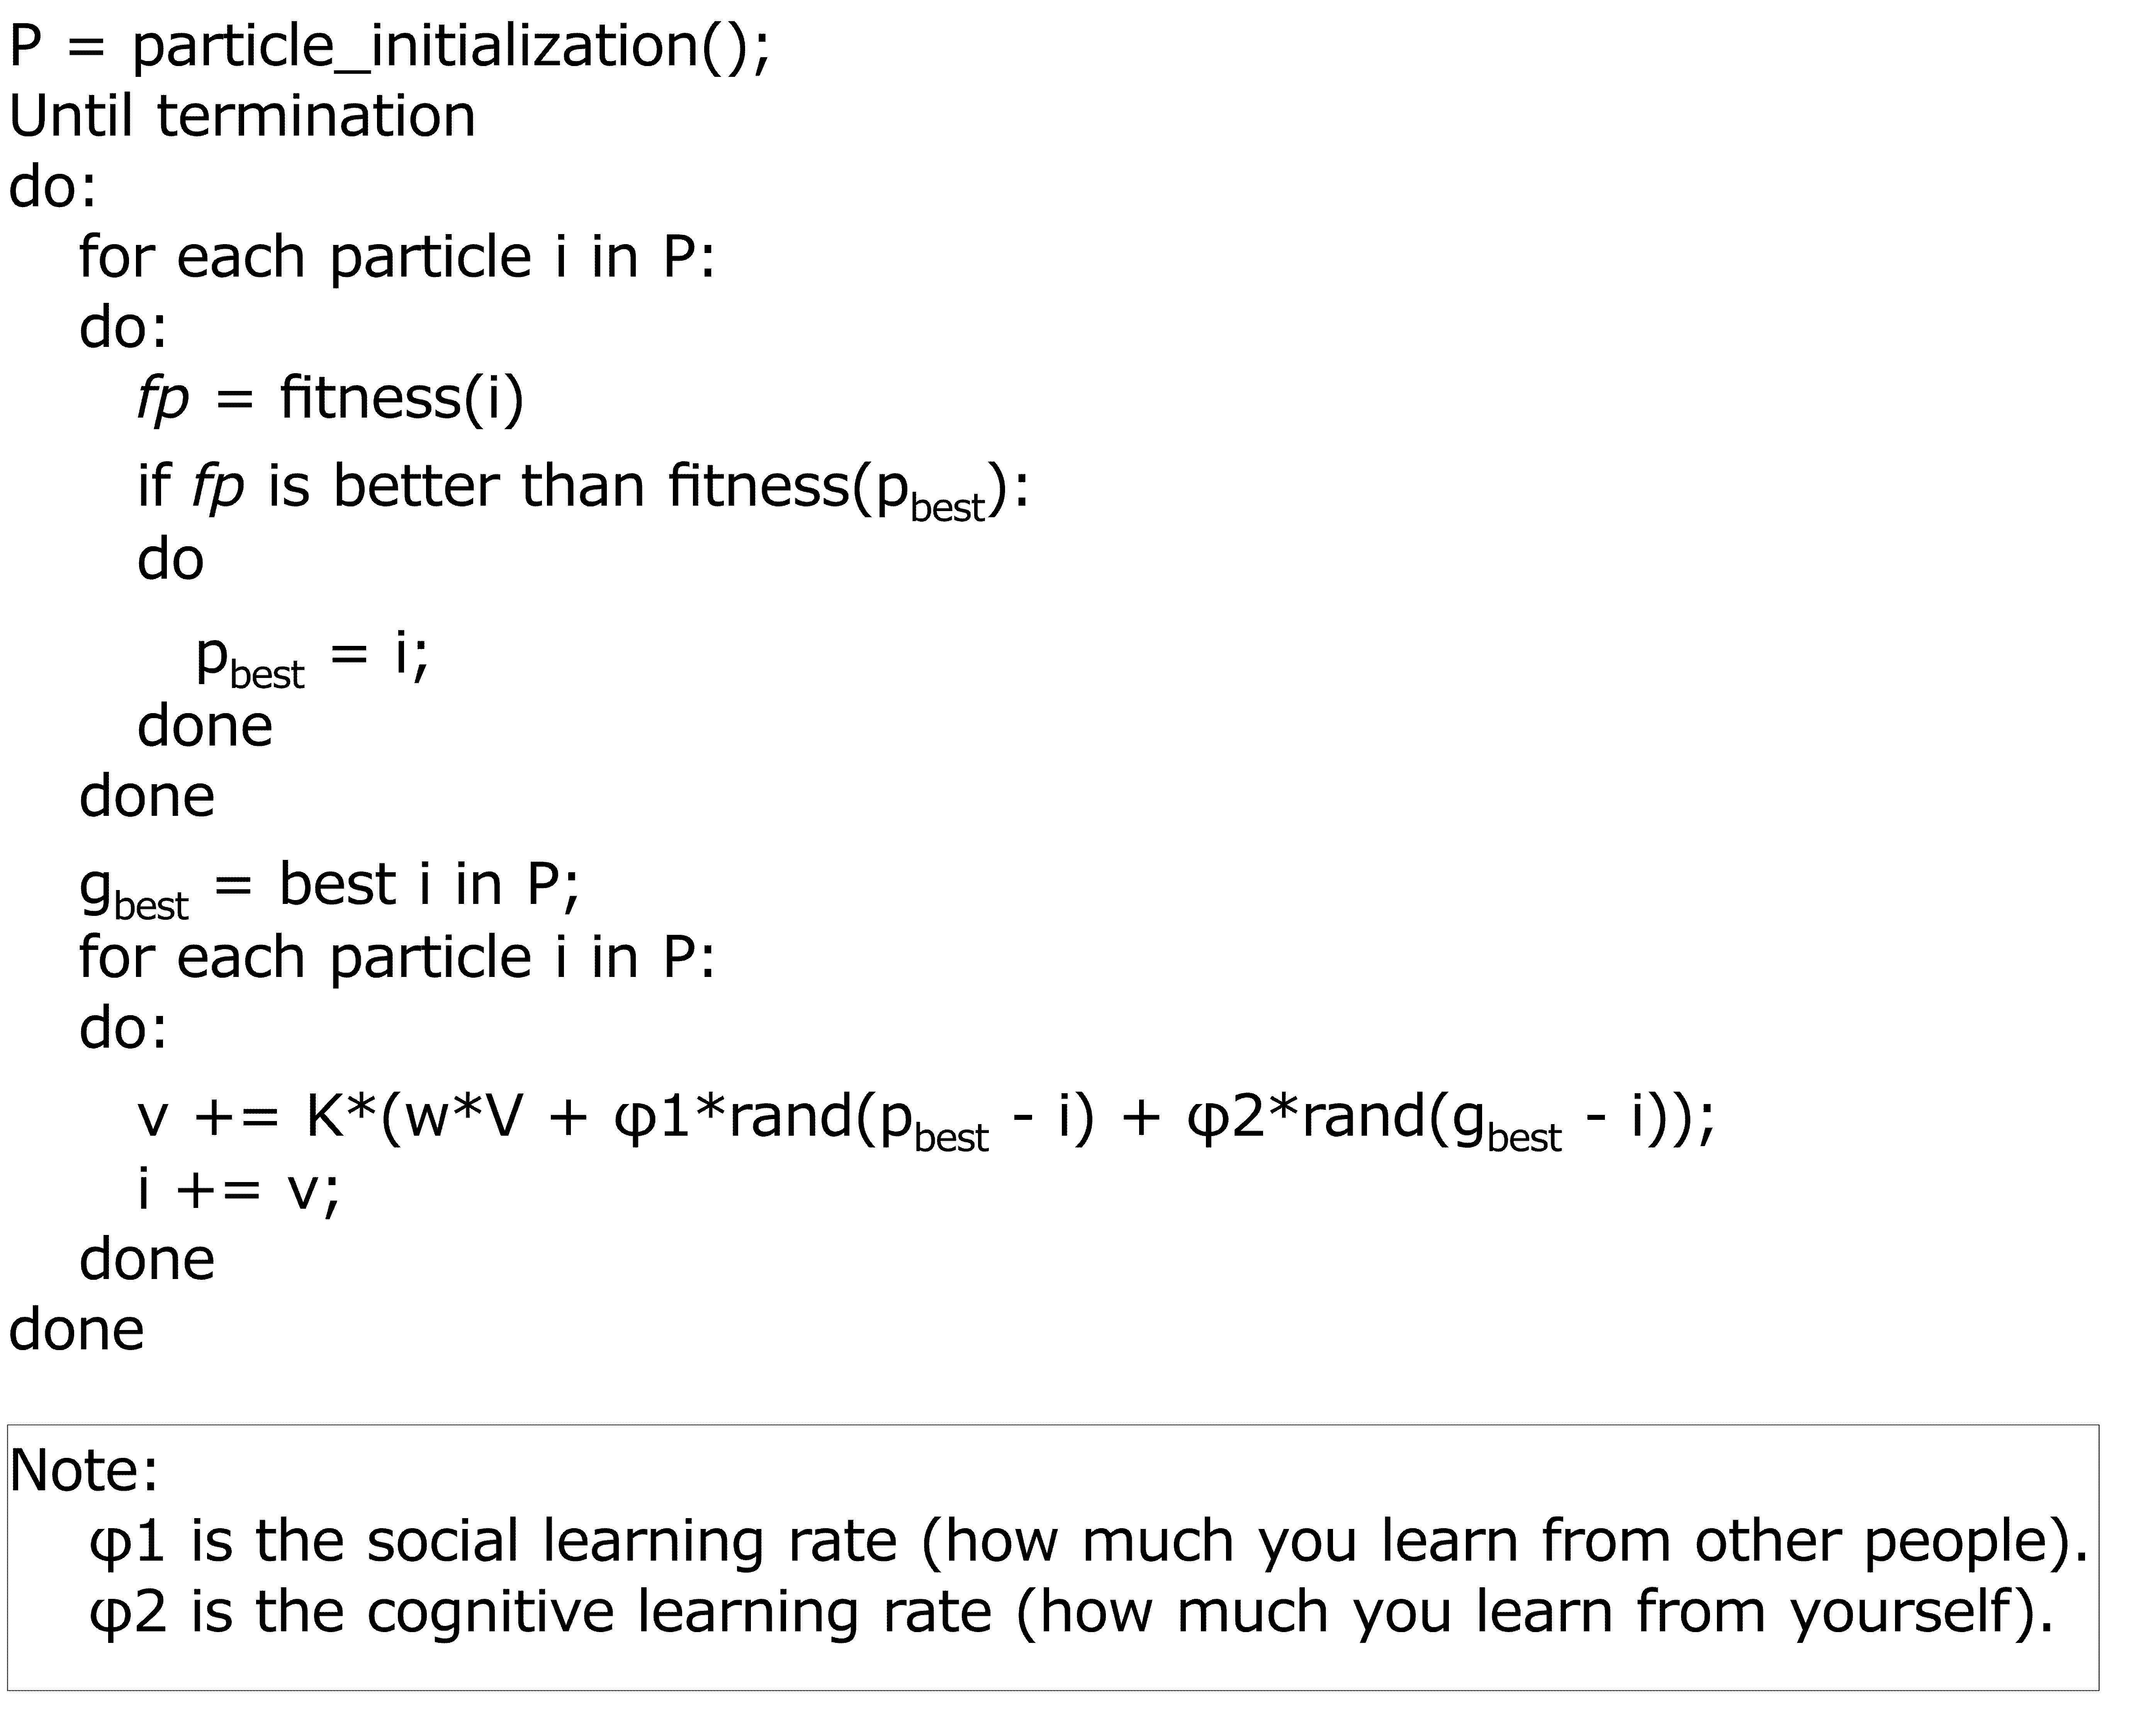
\includegraphics[width=\linewidth]{figs/pso_pseudo.png}
% \caption{Pseudocode for a basic PSO.}
% \label{fig:pso_pseudo}
% \end{wrapfigure}

\begin{figure}[!b]
\begin{minipage}{0.5\linewidth}
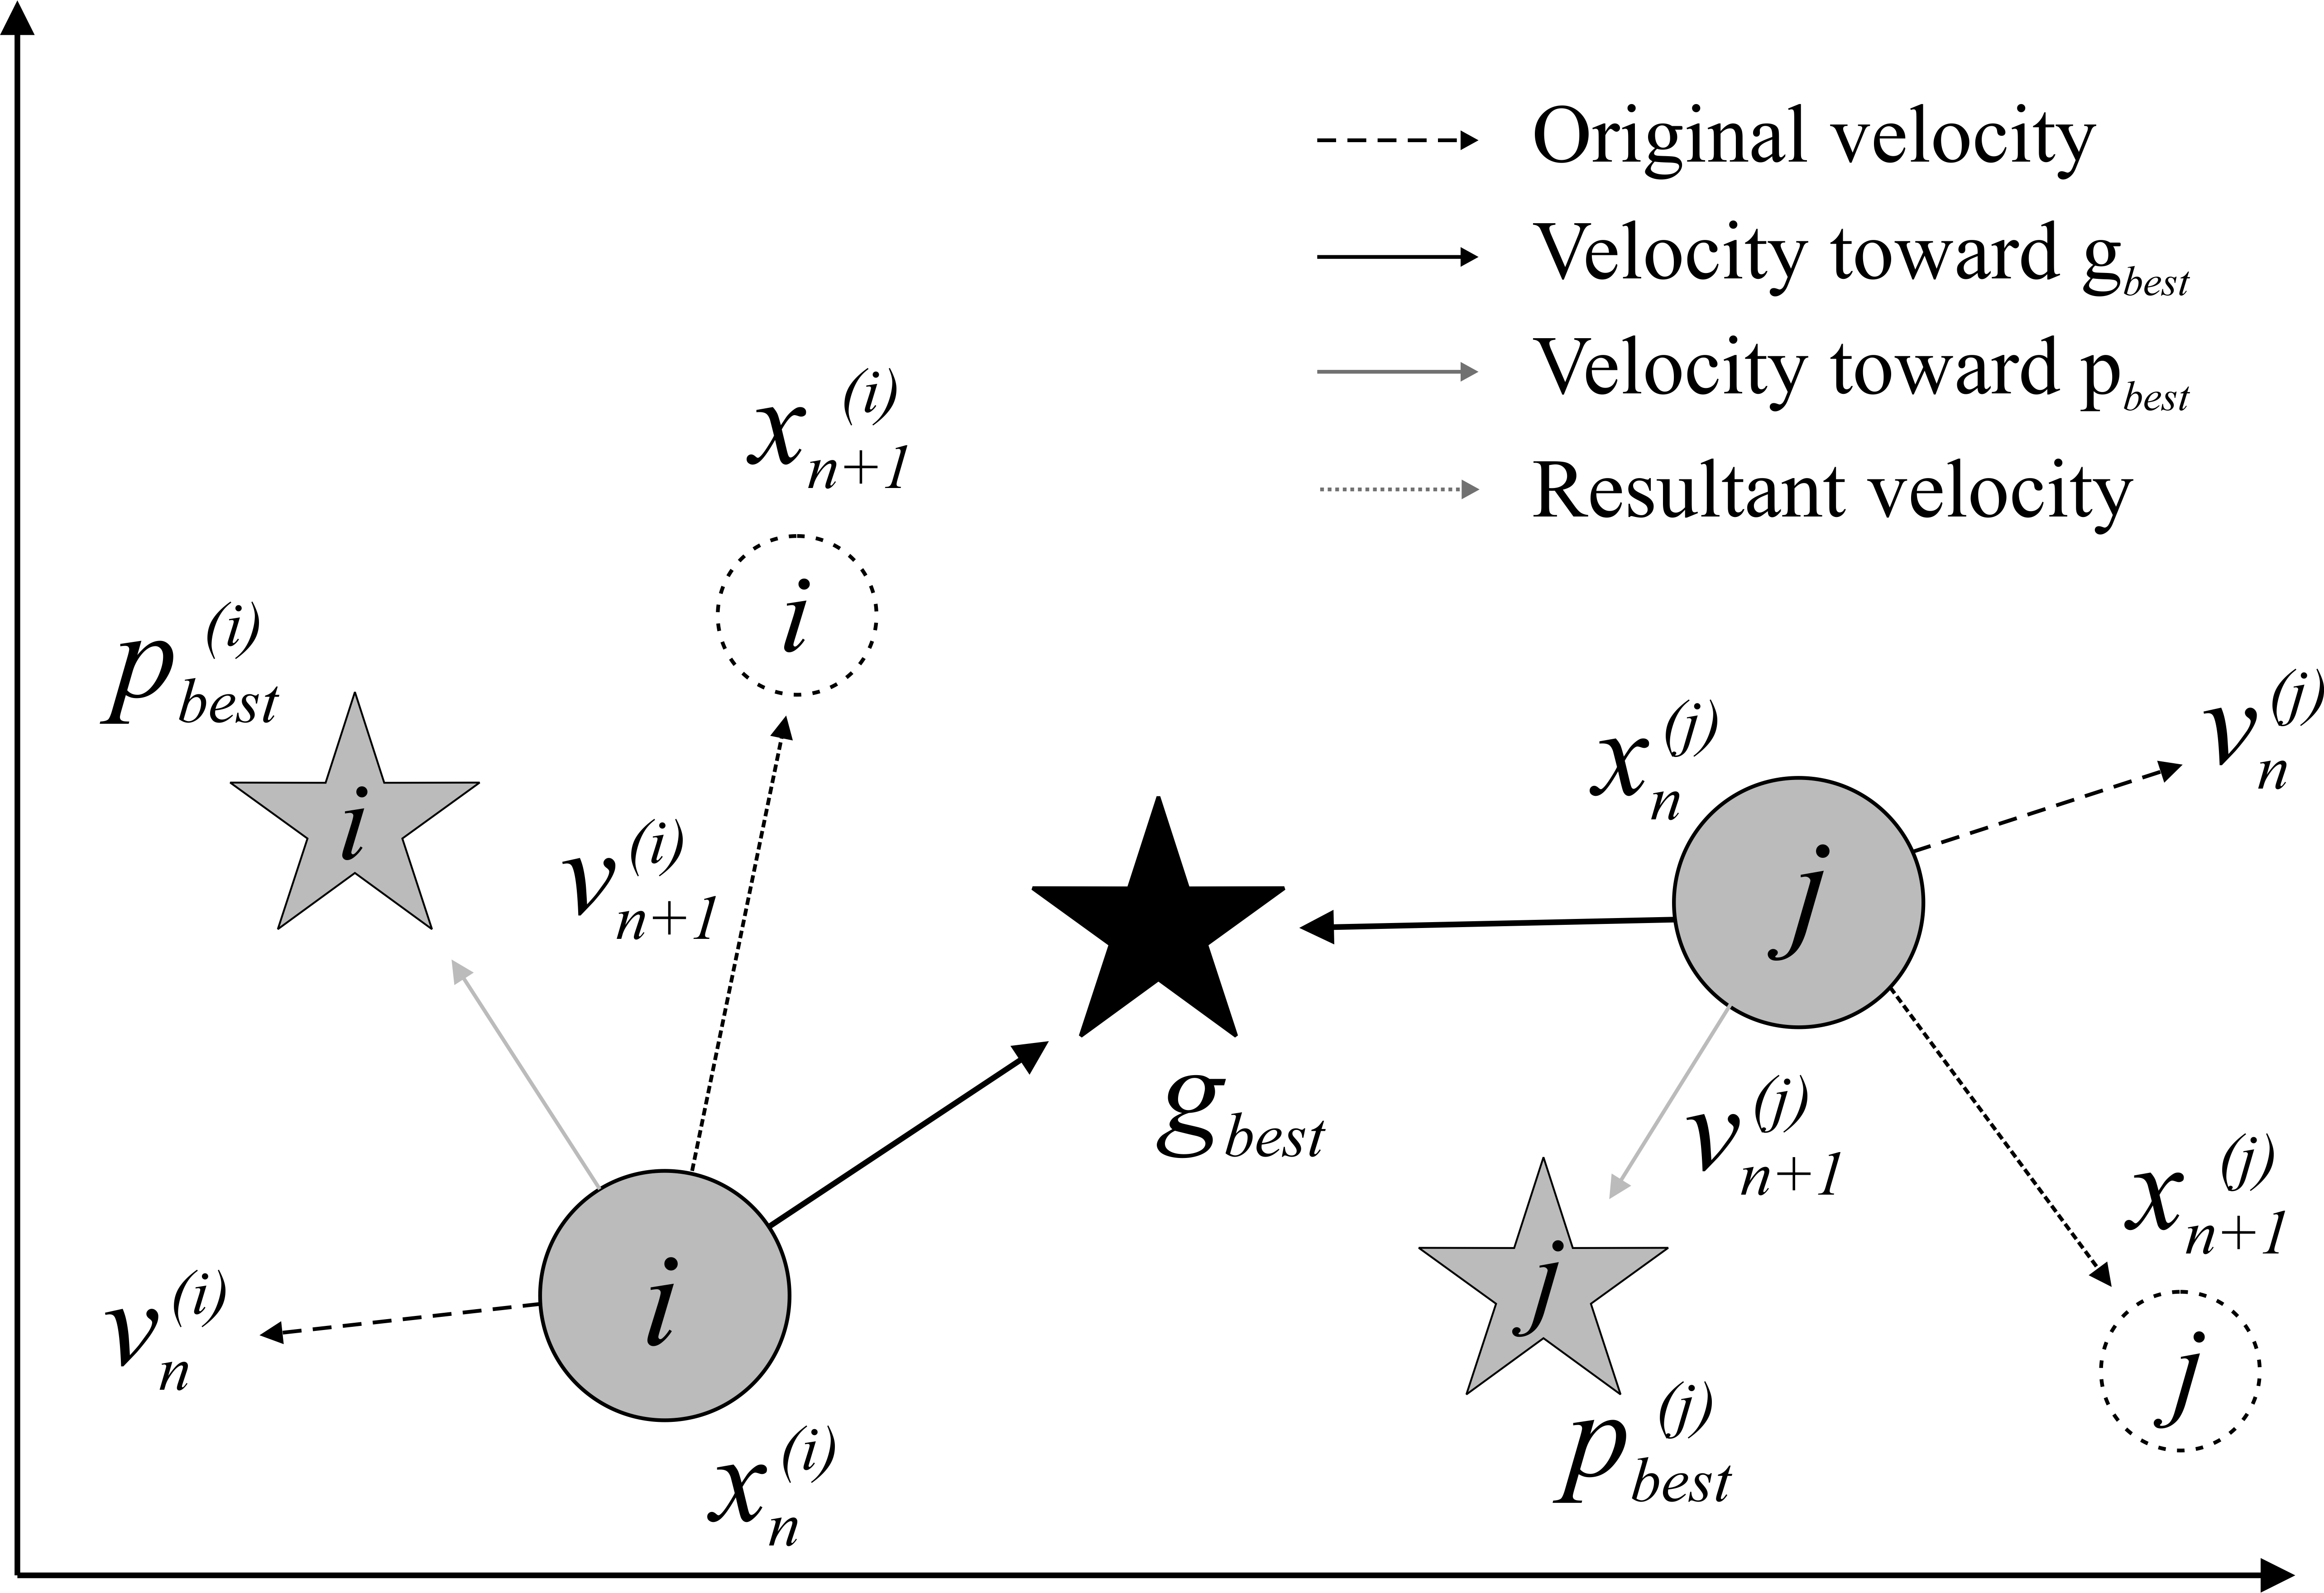
\includegraphics[width=\linewidth]{figs/pso_demo.png}
\caption{Mutations in PSO.}
\label{fig:pso}
\end{minipage}~~~~\begin{minipage}{0.5\linewidth}
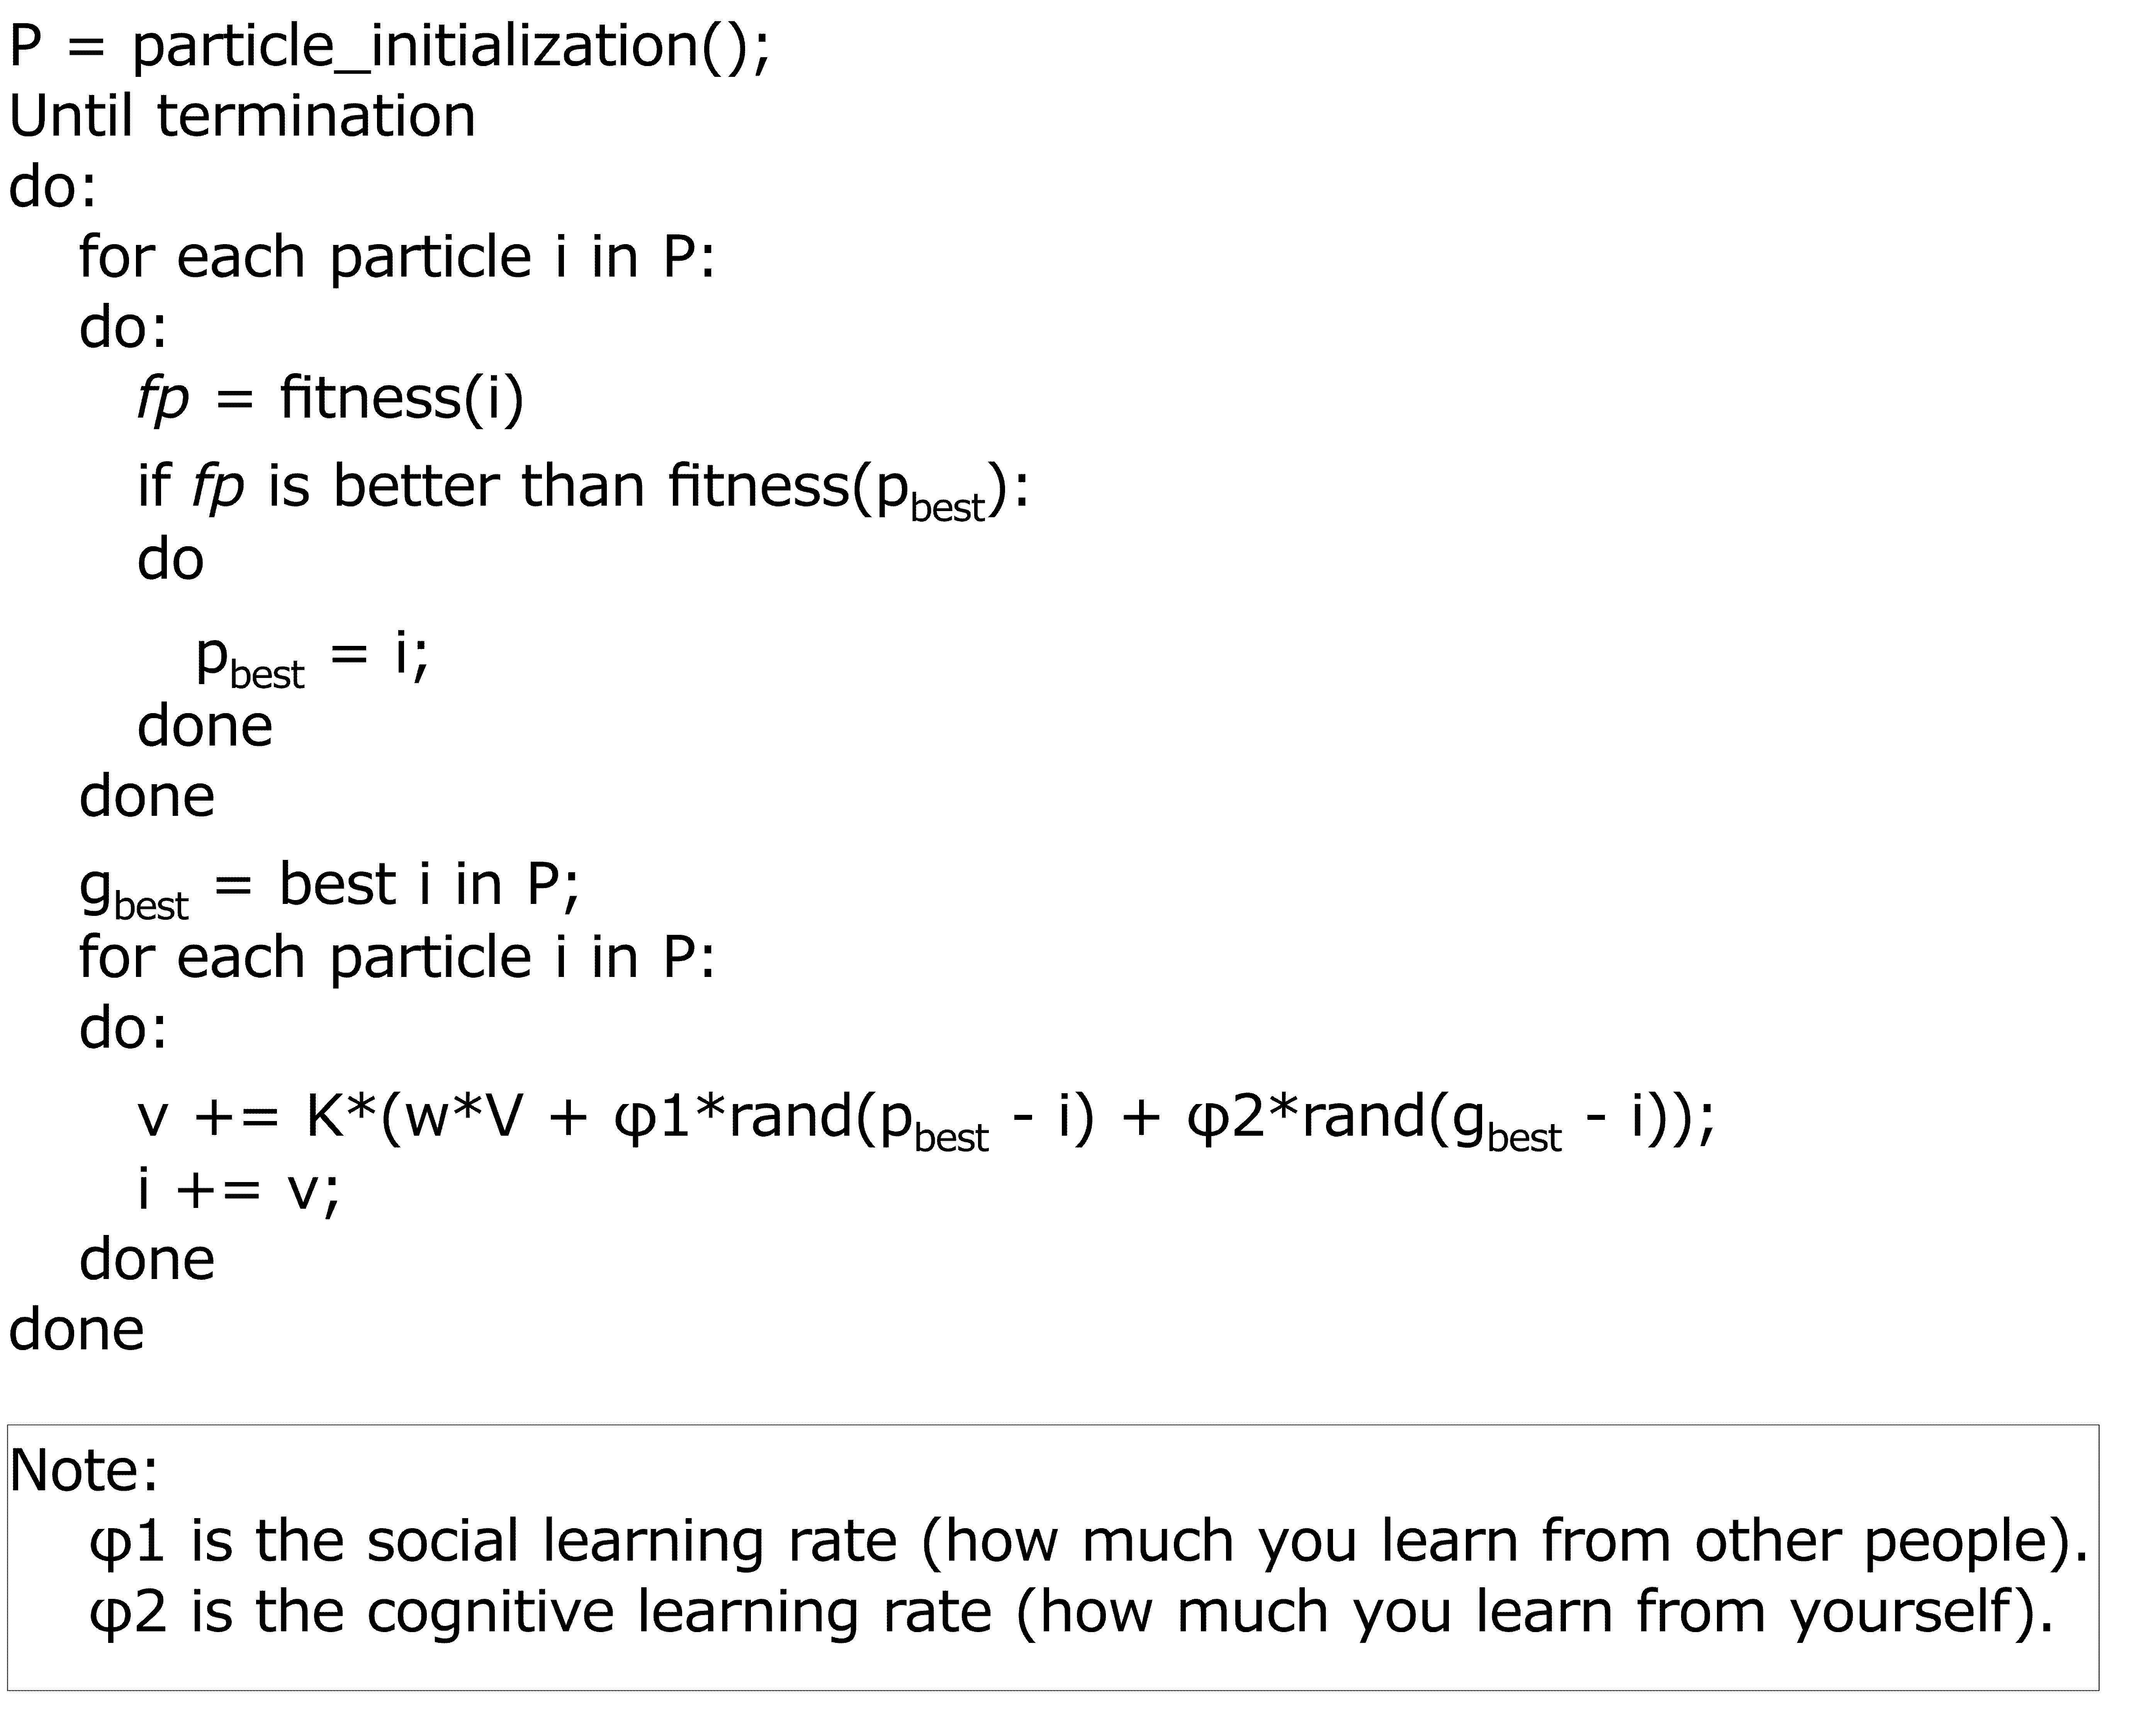
\includegraphics[width=\linewidth]{figs/pso_pseudo.png}
\caption{Pseudocode for a basic PSO.}
\label{fig:pso_pseudo}
\end{minipage}
\end{figure}

% \begin{wrapfigure}[15]{R}{0.4\textwidth}
% 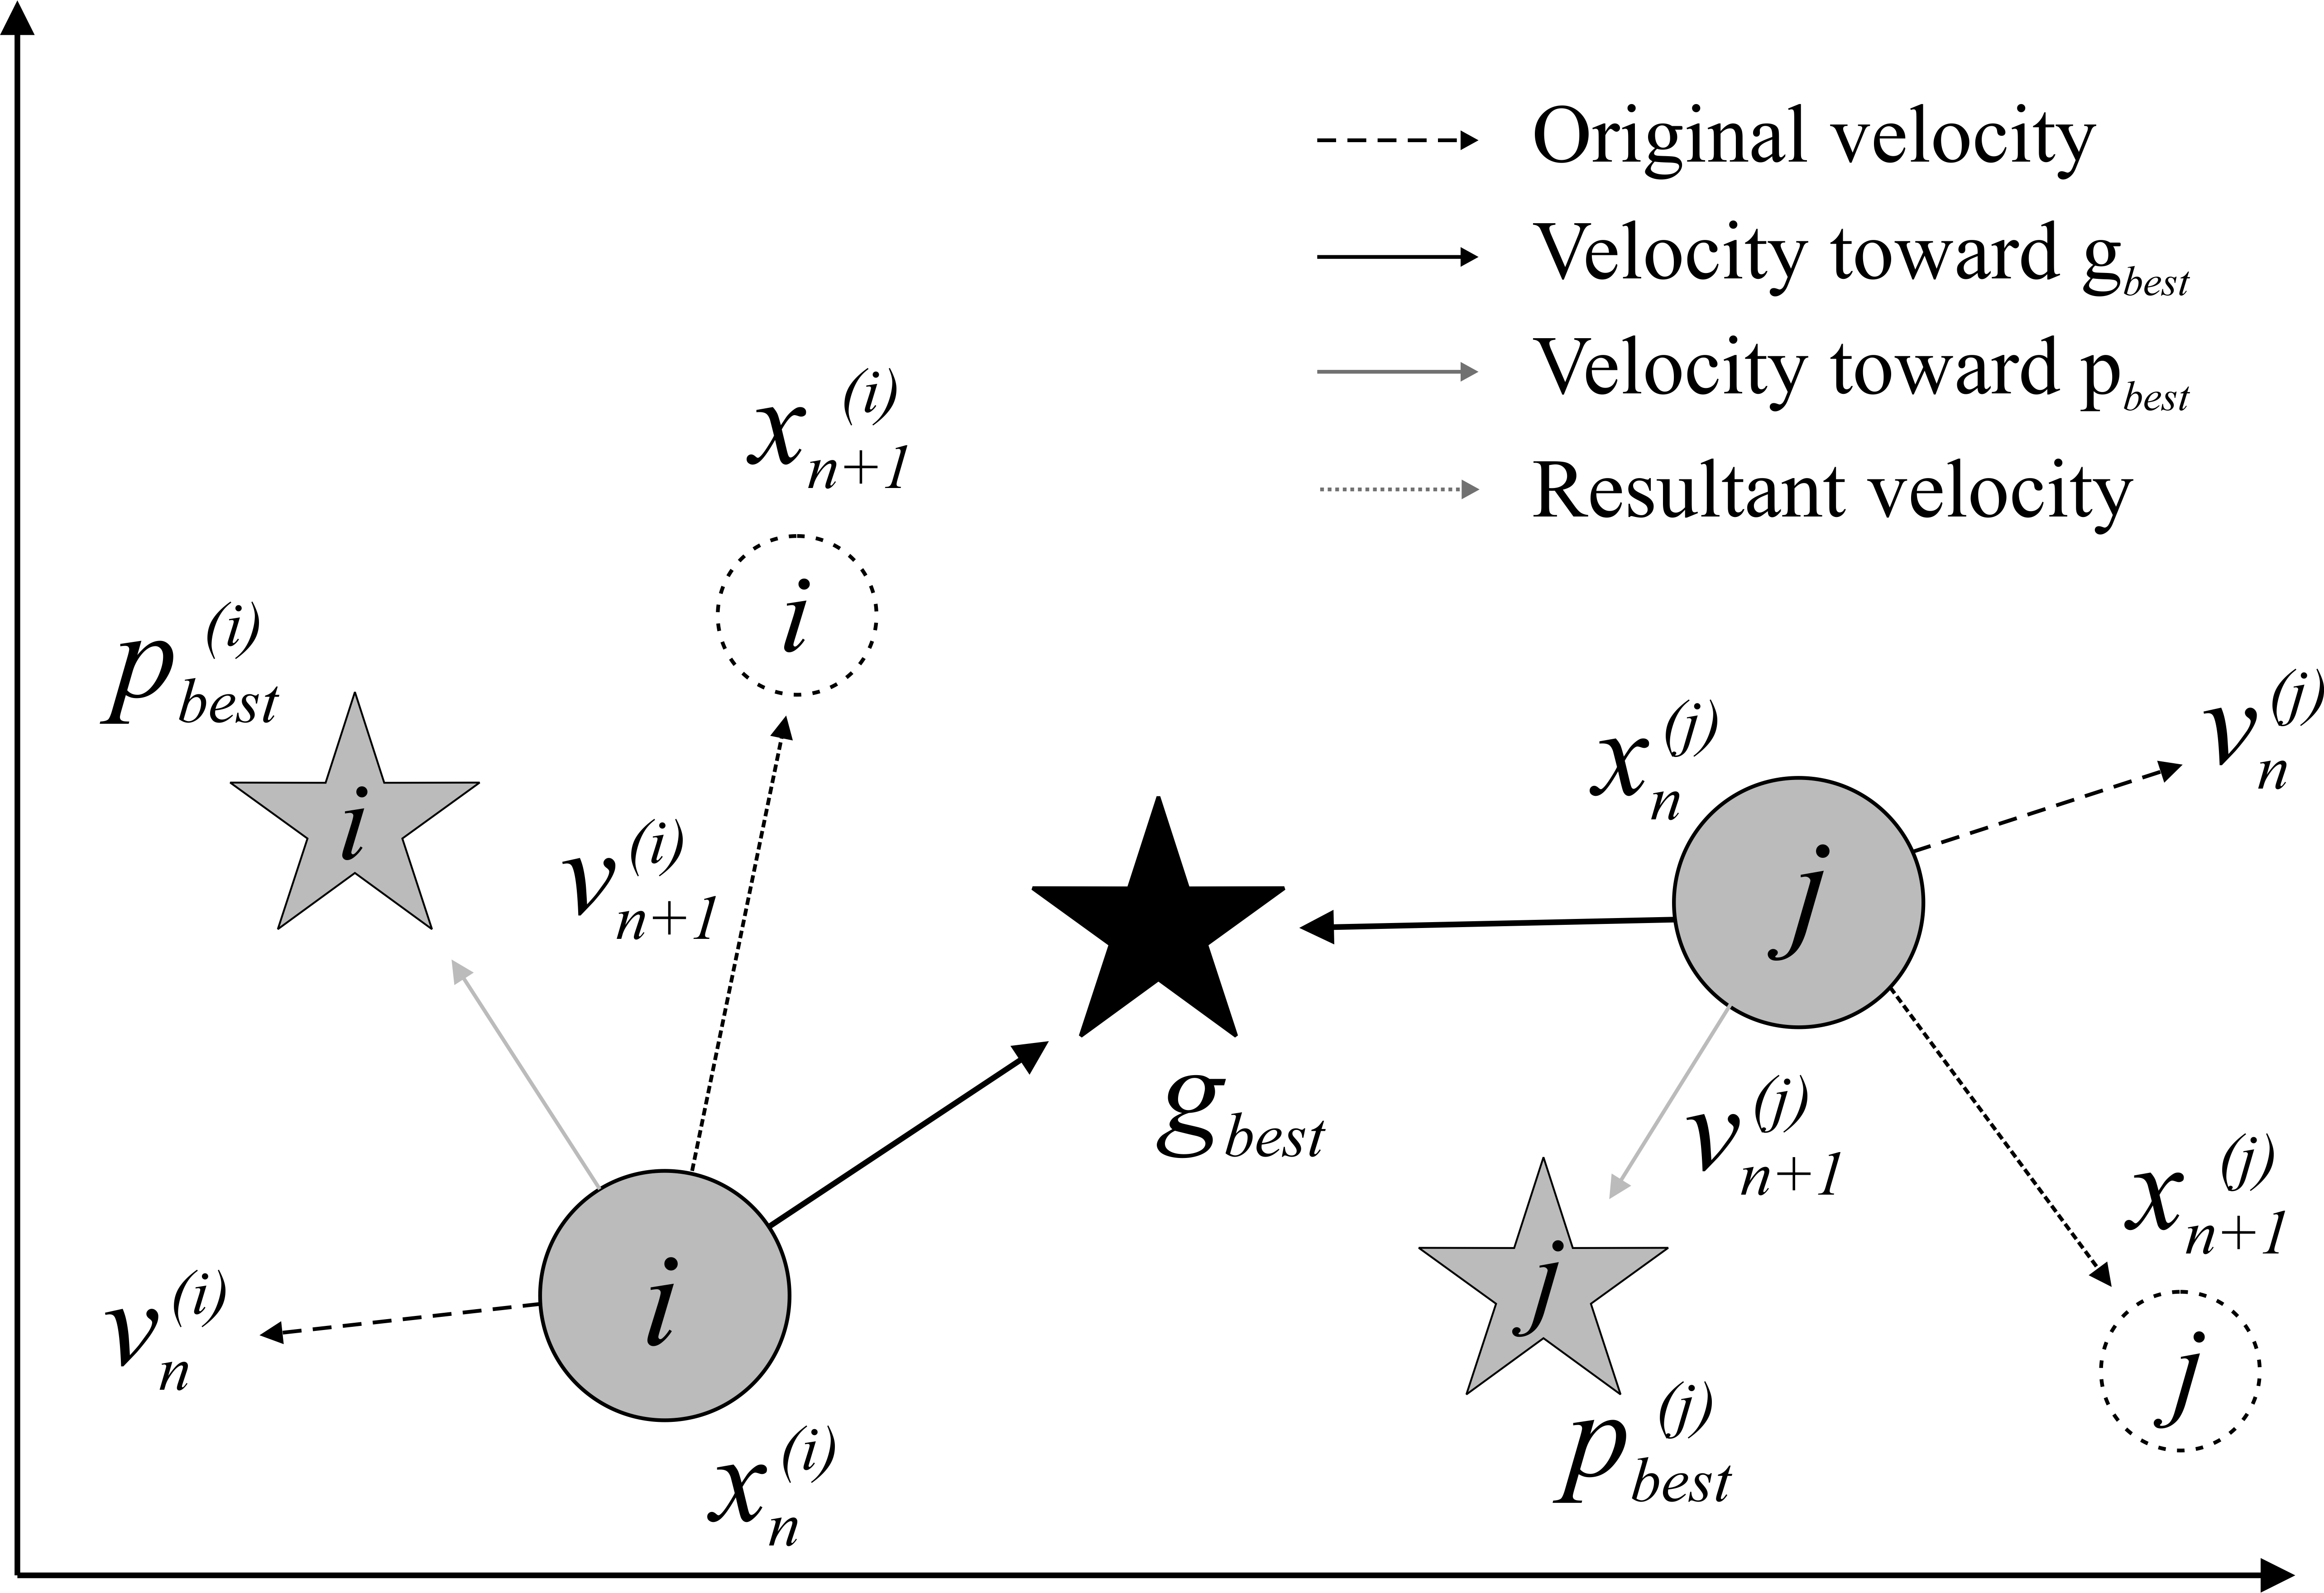
\includegraphics[width=\linewidth]{figs/pso_demo.png}
% \caption{PSO uses sociocognition to mutate its particles. Each particle $i$  mutates in the direction
% $v_n^{(i)}$ while also pulled towards
% (1)~the best idea it ever saw in the past $p_{\mathit{best}}^{(i)}$
% as well as (2)~the best idea ever seen by the community 
% $g_{\mathit{best}}$. As a result, the particle $i$ is redirected towards $x_{n+1}^{i}$.}
% \label{fig:pso}
% \end{wrapfigure}



Our intent is to use stochastic algorithms to learn rules that satisfy the optimization problem described in {\bf \S{3}}.
As to the mutation method, referring to \fig{pso},
each particle $i$  in the swam has
its current mutation  direction
$v_n^{(i)}$. That particle is   also being pulled towards
(i)~the best rule it ever saw in the past $p_{\mathit{best}}^{(i)}$
as well as (ii)~the best rule ever seen by the community 
$g_{\mathit{best}}$ (this best rule is marked by ``{\LARGE $\star$}'' in \fig{pso}. 
As shown in \fig{pso_pseudo}, the pull is determined by  a social cognition factor  $\phi_1$
(that controls how much we learn from others) and
 a cognitive learning rate $\phi_2$ (that controls how much we learn from ourselves).
As a result, the particle $i$ is redirected towards $x_{n+1}^{i}$. For further technical details on our PSO approach, see \tab{arch}:

\begin{table}[!t]
% \footnotesize
\caption{To apply PSO to planning association rules, we need to define (A)~what is a particle; (B)~how to determine when one solution is {\em better than} another; (C)~{\em direction of mutation} of a rule;
and (D)~how to nudge the direction by adding in another rule. }\label{tab:arch}
{ 
\begin{tabular}{|p{.99\linewidth}|}\hline

{\em (A) What is a particle?}
A particle  holds two planning association rules: {\em current} (which is being actively mutated) and  {\em best} which is a copy of the best current planning rule seen so far.
 Particles
also hold a list of sorted ranges, described below. At each step of the SWARM, the current rule is mutated using   ``direction of mutation'' (shown below).
\\\hline


{\em (B)~When is one rule better than another?}  This question is answered by a {\em domination predicate} that reports
one item in a multi-objective space is better than another. More precisely, we define ``better'' via  using Zitler's indicator
dominance predicate~\cite{zitzler2004indicator} that says rule
   $x$   is better than rule  
   $y$ if  
   $M(y,x) > M(x,y)$
   where \mbox{$M(x,y) = \sum_j^n -e^{\Delta(j,x,y,n)}/n$}
 and \mbox{$\Delta(j,x,y,n)  =  w_j(o_{j,x}  - o_{j,y})/n$}.
In these expressions,
 $w\in \{-1,1\}$   represents the $n$ objectives that need to be minimized or maximized. Also, 
 $o_x, o_y$ are the objective scores associated with $x,y$; i.e. the 
  $(o_x,o_y)\in\{I,O,E,D_i\}$ goals from {\bf \S{3}}.
\\\hline
{\em (C)~What is a rule's ``direction of mutation''?}
Rules mutate in the direction defined by weights on a list of ranges.  
Given a set of records, we  compute the {\em domination count}; i.e. using the Zitler predicate, for each records $x$ count how many record $y$ are dominated by  this row.
Next, we discretize  the numeric values in those records by   (a) sorting the values then (b) recursively finding the splits that minimizing the expected value of the standard deviation of the domination count (using the  CART feature selection rule~\cite{breiman1984classification}).

~~~~ Each   symbolic range and discretized numeric range is then weighted. Ranges are selected stochastically as follows.
Compute the CDF (cumulative distribution function) for all the ranges, sorted by those
 weights. 
 For $A$ attributes, add   $A$  ranges to a rule via  a binary search over the range CDF looking for the
 range/attribute pair associated with the   random number $0 \le R \le W$.

~~~~This search will select between $0$ to $A$
ranges for each attribute (so attributes whose ranges are all ranked lowly will rarely be selected). Attributes that are not selected by this process are not
added to a particles {\em current rule}.   Attributes with more than 1 selected range become   disjunctions. 
Clearly, this  CDF search will tend to select attribute ranges from the ranges with largest weights. 
 \\\hline
{\em (D)~How to nudge the direction by adding in another direction?}
To nudge the mutation direction of   rule, we compute the weighted sum of the range weights from two rules (and if a range is in one rule, but not the other, then it has a weight of zero). As seen in \fig{pso_pseudo}, that combination is controlled by the variables  $K,~\phi_1,~\phi_2$
where 
$K$ is a constriction factor to damp escalating velocities; and
 $\phi_1,\phi_2$ control the relative
weightings given to the locally and globally known best solution.
Carlisle \& Dozier~\cite{An01}    $\phi_1$ = 2.8; \mbox{$\phi_2$ = 1.3} (i.e. listen to your own experience about twice as much as that of your fellows).
\\\hline
\end{tabular}}

\end{table}
 
\head{5. RESEARCH PLAN}
In the above we motivated a two-part architecture: (a)~CrossTREE to generate a set of (possibly good) recommendations; then (b)~PSO to take advantage of patterns of usage in how
 developers use the CrossTREE recommendations. 
 This section describes our plan for using this architecture to test the core    hypothesis of this work; i.e.
\begin{center}
 {\em RQ1:  Are human-augmented data miners ``better'' for software   analytics?}
 \end{center}
 
 
\noindent
{\bf Task0: Evangelizing } {\em (a.k.a. Beating the drum.)}

Recalling the discussion around \fig{venn}, we will use feedback from live projects to tune
our learning methods. To gather that feedback, we will see what changes result from posting recommendations
from CrossTREE into the Github issue tracking system.

Other researchers~\cite{theisen2017risk} report that such a ``post an issue and see what happens'' tactic is an effective experimentation  for  teams that communicate via Github issue reports. Nevertheless, it would be prundent to   evangelize our work within the software developer community since, if that were done, developers
might look twice at issues   posted from some source called ``CrossTREE quality system''.

We anticipate no difficulties in visiting local software organizations
and evangelizing this project to a very large local population. It turns out that at NC State University, evangelizing to a large developer community is particularly
easy. NC State University is located 20 minutes away from Research Triangle Park (RTP),
home to 
numerous organizations engaged in extensive software
development including
(a)~SAS,   (b)~NetApp, (c)~EMC Corporation, (d)~Credit Suisse First Boston,  
(e)~the second largest IBM operation 
in the world (smaller only than the one in India)
with 11,000  local employees
and (f)~Cisco Systems' largest campus outside of
Silicon Valley with 5380 employees.  Also, nearby is the corporate headquarters
of Red Hat software,  Lexis Nexis' national   Technology Center, and the ABB Research Center. 
% All these organizations make extensive use of a similar
% tool stack (Github, Jira,   Travis CI) and the standard languages seen in 
% the continuous operations ecosystem (Java,Node.js,  Go, PHP,  Swift,  Python,  Ruby  Sinatra, Ruby on Rails). 
% This convergence of technologies has lead to the emergence of a new generation tools with wide application to
% many software projects. For example, the cloud platform used in this research (and shown
% in \fig{bluemix} is built and maintained  by one of the organizations listed above.
% PI Menzies already has  extensive contacts with that community and,
% in the period 2015 to 2017,   received  \$325K in gift money from these organizations
% to work on  their software analytics projects. 
% PI Menzies regularly publishes papers with  research-active members of that industrial community;
% e.g. see ~\cite{krishna2016bigse,yu16} and the two ICSE SEIP'18 submissions currently under development.  
% % More importantly:
% \bi
% \item Many students from NC State take jobs in the local software industry;
% \item
% Four of PI Menzies'  Ph.D. students students work as interns with these organizations-- and
% two of those students work 
% directly with the team maintaining the cloud platform used for this work.
% \ei
 
\noindent
{\bf Task1: Sanity checks} {\em (a.k.a. The best thing to do with some data is throw it away.)}


% \begin{figure}[!b]
    \centering
    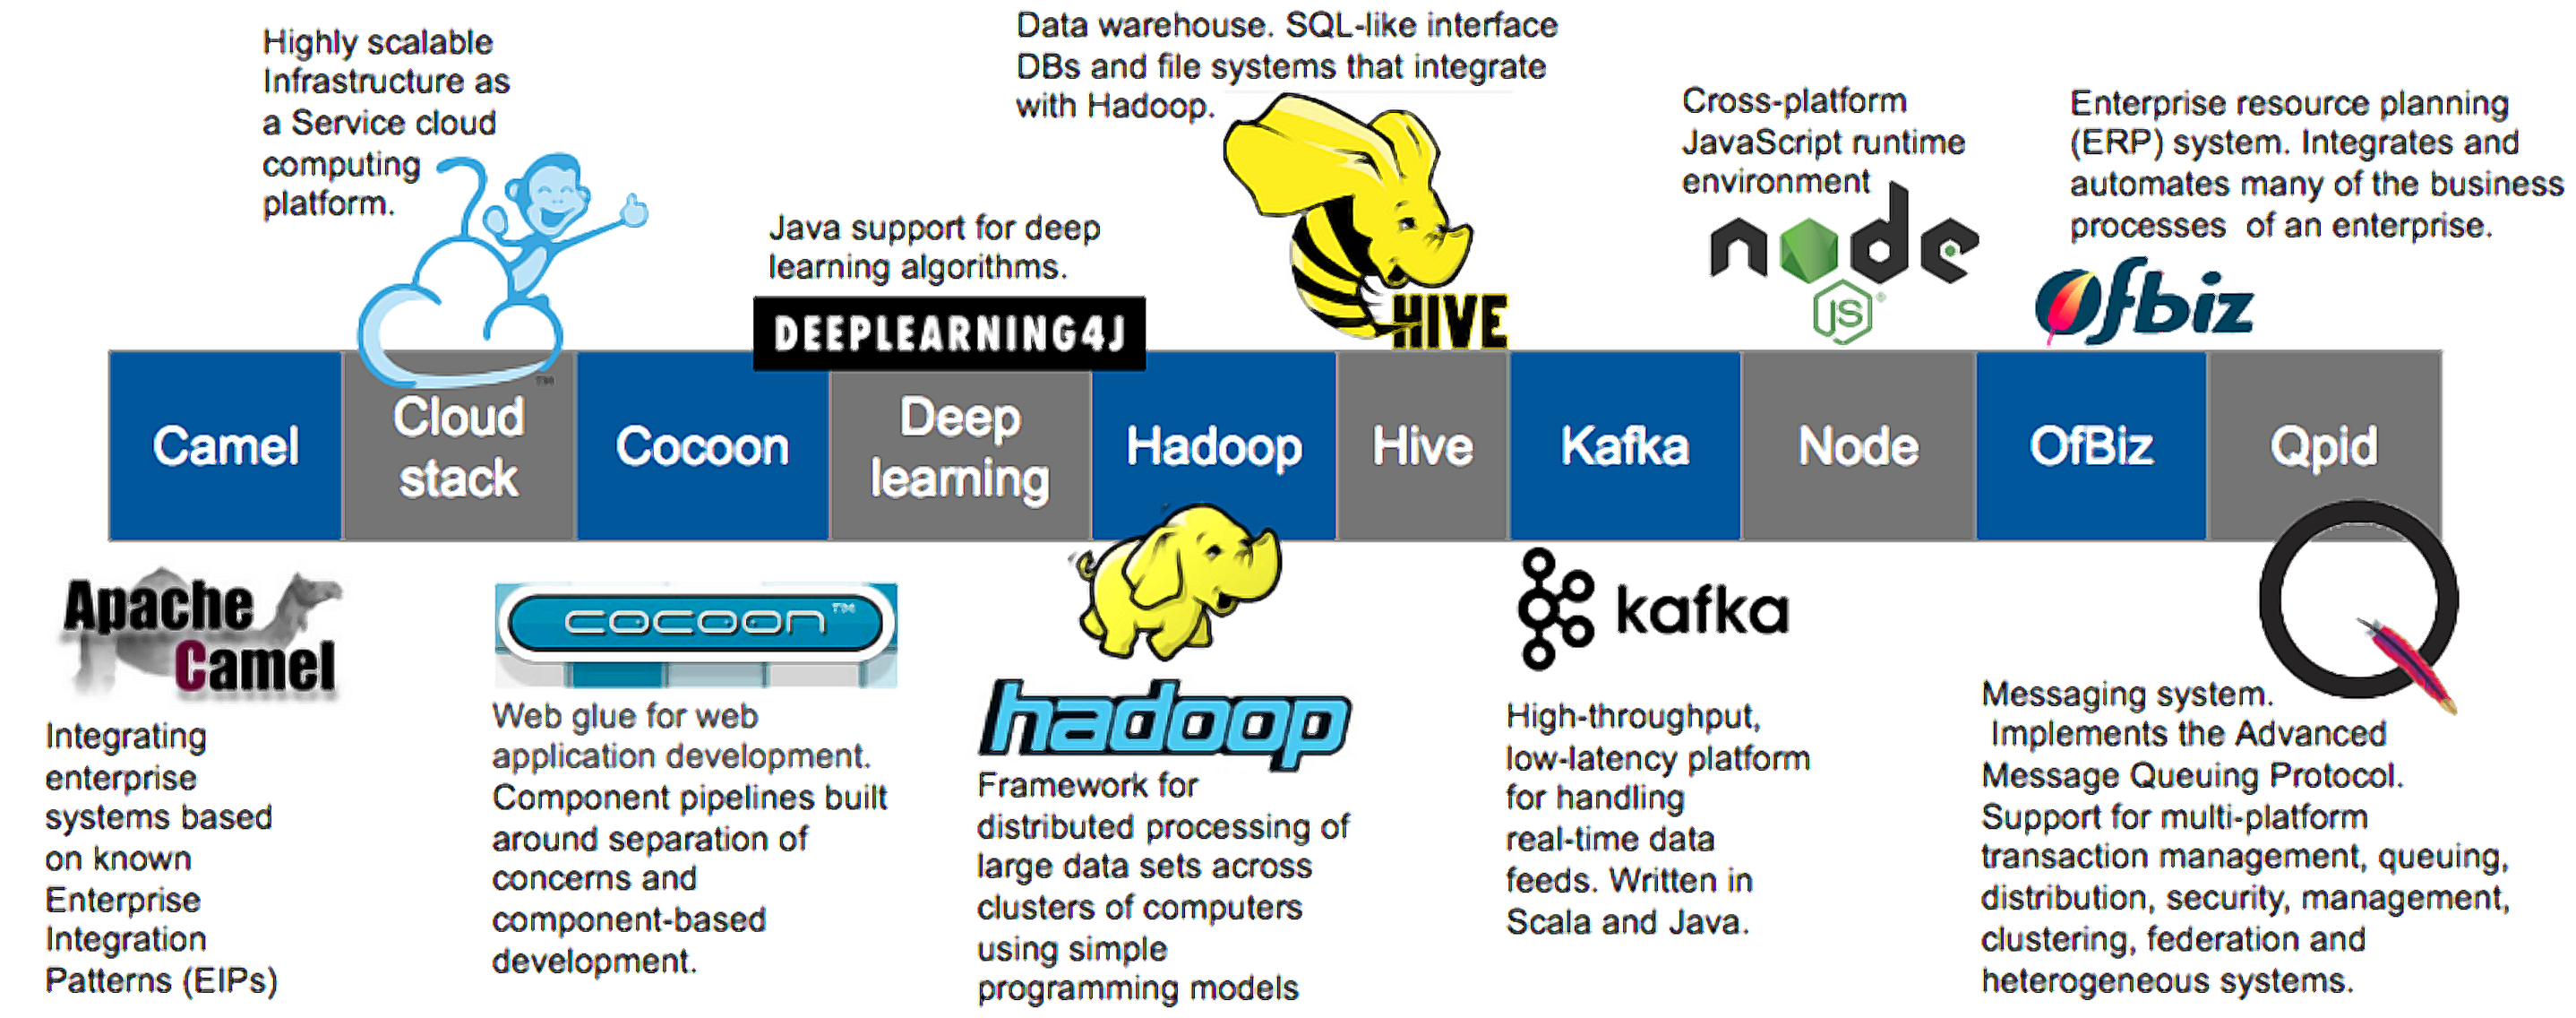
\includegraphics[width=\linewidth]{figs/projects.png}
    \caption{This project will use data from many open source projects, including the above.}
    \label{fig:projects}
\end{figure}


The cloud platform used 
for this work has already ingested Github/ Jira/ Travis CI  data from
538 in-house projects.
and over 1100 open-source projects
marked by Github as ``most trending''. A small sample of those projects are listed in \fig{flow}
 (and note that, for confidentiality reasons,
we cannot list details on the proprietary projects we can access within this cloud platform).
 

Bird et al.~\cite{bird2009promises} caution that many  Github projects are mere ``hobby'' projects and these should not be used as part of any serious research project.
They offer a list of ``sanity checks'' for selecting Github projects. Based on experience with this  data, we have slightly
augmented those sanity checks. \tab{sanity} shows the results of applying those sanity checks to our 1646 projects. Note that even after culling ``hobby''
projects, we are still left with hundreds of open source and in-house projects to use in this research.
 

\begin{wraptable}[13]{r!}{0.6\textwidth}
\footnotesize
\centering
\caption{Sanity checks. Starting with 1108+538  open source+in-house projects, we discard  projects that {\em fail}
any of the LHS tests to arrive at 661+171 projects.}\label{tab:sanity}
\begin{tabular}{|l|r|r|}
\hline
Sanity check & \multicolumn{2}{c|}{\#discarded projects}                     \\ \cline{2-3} 
\multicolumn{1}{|c|}{(discard projects that violate these tests) }                              & \multicolumn{1}{l|}{In-house} & \multicolumn{1}{l|}{Open-source} \\ \hline
\# Pulls \textgreater 0                             & 35                            & 54                              \\
\# Issues \textgreater 10                            & 60                            & 89                              \\
\# Commits \textgreater 20                          & 68                            & 96                              \\
\# Developers \textgreater 8                        & 47                            & 67                              \\
\# Releases \textgreater 0                          & 136                           & 44                              \\
Project time frame \textgreater 1 year              & 12                            & 46                              \\
Projects doing only software development            & 9                             & 51                              \\ \hline
%Total Projects                                      & 538                           & 1108                            \\
Surviving projects                                  & 171                           & 661                             \\ \hline
\end{tabular}
\end{wraptable} As to other data cleansing tasks, we will perform {\em column pruning} via the range generation method of \tab{arch} (part C),
and {\em outlier removal} via the clustering methods described below in {\bf Task3}.


 
\noindent
{\bf Task2: Goal Stratification} {\em (a.k.a. We cannot do everything, but we want to do many things.)}
 
 Recall from  {\bf \S{3}} that  the goals of this work are to learn software quality plans that minimize $I,O$ and maximize $E,G_x$. 
As shown in \tab{metrics},
our data set supports
exploration of many external attributes, any one of which could be the quality goal $G_x$ we will seek to maximize.
% That said, the  data we are exploring is   vast and the patterns of \fig{venn} are only meaningful if developers are changing code
% in order to achieve some goal that they actually care about.
% Hence, for this work, we will restrict our search for software quality goals $G_x$ for
% which it is known that some   manager or developer or active research
% group is currently exploring. 

% It turns out, even with that restriction, there are many such quality issues.
For the last two years, 
PI Menzies and his graduate students have  regularly interviewed studies with project
managers and developers to find the issues that drive their policy decisions.
and how those goals can be assessed via data mined from tools like Github, Jira, Travis CI, etc. 
In these sessions, we asked managers and developers ``what do you want to do, and do better?''. Their answers are as follows.
In this first task we will hold extensive on-line surveys   and in-person meetings to check the currency of the above list, perhaps to even expand it.
\bi
\item[$G_1=$]
Reduce defects~\cite{moniruzzaman2013comparative}; 
\item[$G_2=$]
Decrease development effort~\cite{sarro2016multi,menzies2017negative}; 
\item[$G_3=$]
Reduce issue resolution time~\cite{rees2017better}; 
\item[$G_4=$]
Rank issues such that more important ones get resolved faster than more trivial problems~\cite{moniruzzaman2013comparative}; 
\item[$G_5=$]
Decrease the impact of new personnel to project productivity~\cite{brooks1975mythical}, e.g. by learning a threshold below which it is safe to add new programmers to a project~\cite{agrawal17time};
\item[$G_6=$]
Increase the use of less-expensive software tools that improve productivity~\cite{bruckhaus1996impact}, or decrease the use of expensive tools that have no discernible
effect on products~\cite{rahman2014comparing}; 
\item[$G_7=$] Providing a proper documentation so that new personnel joining can have reduced ramp up time~\cite{petersen2009comparison}.
\item[$G_8=$]
Assess if it is useful to adopt a Continuous Integration approach~\cite{shahin2017continuous,vasilescu2015quality}.
\item[$G_9=$]
Determine what are the  right rate of releases for a project. 
If too slow  then a vendor might lose their customer base (customers may jump to other vendors offering more novel functionality
faster)~\cite{chen2015continuous}.
\item[$G_{10}=$] Provide techniques that can make software development be more language-agnostic~\cite{mens2005challenges}.
\item[$G_{11}=$]
Discover the right time for adding personnel to a project. If removed too early then the current project will suffer. If removed too late then too many programmers will be working on 
current projects (and newer work will be unnecessarily delayed)~\cite{rodriguez2012empirical}.
\item[$G_{12}=$]
Learn different ``bad smells''. For e.g.,
    \bi
        \item[$G_{12a}=$] Program features that are usually associated with code problems.
        \item[$G_{12b}=$] Process features that are usually associated with late or otherwise challenged projects. Further, an example of this might be a team  where most of the changes are (a)~made by a few  ``hero'' programmers~\cite{agrawal17hero} or (b) novice developers are likely to introduce defects than those produced by subject matter experts.
    \ei
\ei
There are two encouraging aspects to the above list. Fristly, 
we already have preliminary results on some of the above (see references to our work at $G_3,G_5, G_{12}$).  
That is, we already know that which data source is a rich source of insight into software engineering.
% \item
% We have discussed this list with several industrial cloud-based development teams. While not all goals are interesting
% to all parties, there is much overlap in their current interests.
Secondly, 
Many of these goals are also active research areas in the literature (see all those with references). For those
goals we will have ready access to alternate methods (and results from those methods) which we can use to baseline
our results. Also, the presence of those other research results means that we have a publication path for this work
(e.g. ``previously, a team at ABC argued for DEF but using our human-augmented data mining approach we have discovered GHI'').


\noindent
{\bf Task3: Data Stratification} {\em  (a.k.a. Not everything applies to everything. )}
 
Another way to divide this problem is {\em data stratification}. Boehm~\cite{Boehm:2006} strongly
advocates for data stratifications; i.e. not learning on all available data but on targeted subsets.
% A similar conclusion comes from other researchers~\cite{menzies2013guest} including Krishna et al.'s  who comments that
% during   transfer learning  (using data from one project to learn predictors for another)
%  if data
% is divided N ways, then best results for one division come from a poll across (a small number) of nearby divisions~\cite{Me13,krishna2017learning}. 
% There are many ways to divide SE data, some of which are not always productive. For example:
% \bi
% \item
% Dividing software project data via implementation language is becoming less and less useful since many current
% projects now use combinations of languages for different parts of their system.
% \item
% Dividing data into
% open source and proprietary is not always helpful. With Agrawal~\cite{agrawal17hero}, we have found that many 
% of our quality measures are not statistically significantly different between open source and proprietary.
% Further, with He et al.~\cite{he13} note that,  after computing the distance between projects (measured as an aggregate
% over the data from these different projects),   (a)~some proprietary projects are in fact closer to open source 
% projects that other proprietary projects and (b)~best quality estimates for open source projects can sometimes
% come from proprietary projects.
% \ei
Some such stratifications can  be very useful. 
% For example, Agrawal~\cite{agrawal17hero}  reports that if projects
% are sorted via frequency of release, then there are very clear divisions between waterfall-style projects
% (which release rarely) and agile-style projects (that release very frequently). 
Petersen and Wohlin~\cite{Petersen2009} have commented on which context variables to explore when searching through project data.
While we plan to follow their advice wherever possible, their advice has two limits. First, they offer certain pre-defined stratifications for software projects and there is no way for a reader of that work to determine if those stratifications are more useful than some other set. Secondly, given the ever-changing nature of the software landscape, it is likely that new kinds of projects
will appear in the near future. Petersen and Wohlin are silent on how to commission new kinds of stratifications.

Previously we have much success with automatic stratification tools. Such automatic clustering
address our two issues with the Petersen and Wohlin manual clustering approach.
When  clusters are learned automatically,   new kinds of projects are always accommodated;
Also, 
such clusters are always auto-assessed via the clustering creation mechanisms.

The are many other advantages to such auto-clustering.
Firstly, an important data cleansing heuristic is {\em outlier removal}; i.e. only do the reasoning within
similar sets of records. Clustering implements this important data cleansing step since, for each cluster, every other cluster is the outlier.
% Secondly, the rules generated from local clusters
% contain more effects familiar to developers working on projects in those clusters.
Secondly,
if data is stratified automatically via clustering algorithms,
then the resulting models learned per cluster may have similar median performance but
have far less variance than models learned from all the data~\cite{Me13}. 
% Fourthly, During 
% {\em transfer learning} (where data from one project is used to make predictions for another), then
% some subset of those clusters are often an {\em bellwether} (source of exemplar data that applies to other projects)~\cite{krishna2017learning,krishna2017simpler}. 
Thirdly, and
more specifically for this project, such automatically-generated clusters can be used to better define the ``global'' best rule as used by the PSO algorithm defined above. Classic PSO use a global ``best'' from all data. But for data as large as what we are processing, it seems prudent to cluster and redefine ``global'' to be mean ``best within the current cluster''.  Hence, for this work, we propose (a)~running
some incremental clustering algorithm (e.g. mini-batch K-means~\cite{Sculley:2010}, or its
more recent variants ~\cite{Sculley:2010}); then (b)~  running one of our PSO algorithms within each cluster (so in those clusters ``global best'' means ``best in this clster'').
One advantage in restricting PSO to subsets of the data is scalability. Whatever the runtime costs of PSO, by dividing that up and running
in parallel over multiple
tiny regions of data, then this would lead to dramatic speed ups in PSO.

\noindent
{\bf Task4: Data-lite} {\em (a.k.a. Make it run locally.)}

Our initial plan is to make all the above work within the cloud IDE
described in the introduction. That said, for the purposes of micro-experimentation and reproducability,
it would also be useful to perform all the above outside that IDE.

Working outside that IDE is practical and possible. While researchers would lose access to the proprietary projects inside this IDE, they could still access via Github, and associated tools
such as  GhTorrent (ghtorrent.org), and 
Github Archive (https://www.githubarchive.org/) to access much of the information stored in our
cloud platform. However,  are two caveats to that statement. Firstly,
the cloud platform offers extensive access to on-line CPU farms and cloud-based secondary storiage devices; and secondly 
the cloud platform routinely implements extensive joins between Github and other tools  such as the
Jira issue tracking system. Further, the results of those joins are cached and indexed
and made available via APIs. 
Hence, not everything we could do inside the cloud IDE might be 
easily reproducable otherwise. 

That said, we suspect it possible that after some experience with
our kinds of analysis, there will emerge a ``typical set'' of attributes that most often appear in our
planning rules. If such a ``typical set'' is found, then some lightweight collection policies
could be added to projects to collect and cache those sets-- in which case it may well be possible
to optimize for all the goals we are exploring in the cloud IDE without requiring extensive
extensive and expensive cloud-based CPU or secondary storage facilities.

\noindent
{\bf Task5: Execution} {\em  (a.k.a. Ready, set go.)}

Once the data is (a)~cleansed, (b)~sorted into groups reflecting different goals (with spurious records removed), and 
(c)~clustered into groups of records, the next task is to:
\bi
\item
Run CrossTREE;
\item
Which generate recommendations which are posted as issues to developer issue systems;
\item
Then monitor the subsequent changes to the code base;
\ei
Note that one of the reasons we are requesting four years of funding for this work is that, since this task will require
extensive monitoring to future changes in a project, this task will take some
time to complete.

\noindent
{\bf Task6: Evaluation } {\em (a.k.a. Testing {\bf RQ1}.)}

The evaluation criteria for this work was presented above: it was a four-goal optimization problem with the aim
to propose changes that were rarely in the sets $I,O$ (things {\em ignored} by developers, or changes {\em other} than
what was found by our methods) and were often seen in $E$ (things suggested by our tools and {\em endorsed} and enacted
upon by developers) and which had a large beneficial effect on some quality goal $G_x$.
Also, for quality goals that other researchers have explored, we would need to see which of those techniques
we can reproduce and compare with our methods. For example, in recent work where we built predictors for how Github issues
will take to close (using data from the cloud IDE). In our report on that work~\cite{rees2017better}, we showed
that our methods out-performed the prior state-of-the-art in this area~\cite{Kikas:2016}.
Note that with results from our approach, compared to some prior state-of-the-art, we can test our hypothesis that human-augmented data mining methods produce better predictors and planners for software quality. 
\bi
\item For a list of prior results relating to our goals, see the citations in the $G_x$ list shown in {\bf Task2}.
\ei
% The following two results would be very challenging to our research themes:
% \bi
% \item Methods taken from prior results perform better than our CrossTREE/PSO methods. Such a result would cast doubt on the value of our entire archicture.
% \item CrossTREE's recommendations perform just as well as anything generated via PSO. This would tell us that added human intelligence to our artifical intelligence
% methods was {\em not} useful, at least for the architecture studied here. Note that this result would {\em not} prove that all 
% AI was better than human intelligence (Shull et al.~\cite{shull02} offered examples in his prior work where a little human contextual knowledge greatly improved insight from
% automatic tools). But if CrossTREE performs as well as anything else, then it would motivate more resaerch on automatic big data research rather than human-in-the-loop
% reasoning.
% \ei

Other evaluation criteria to be considered are the {\em CPU cost} of our methods.
Many of our recent papers~\cite{chen2017beyond,fu2017easy,nair2017faster,mathew2017shorter,nair2017flash,chen2017riot}, 
and the work of others~\cite{Fisher:2012}, raises concerns about the reliance on CPU-intensive methods.
Such methods complicate reproducability -- an essential part of the scientific methods. Our design, described above, proposes
limiting PSO to just clusters found via min0batch K-means.
Still,  given the large size of of the data set on
the cloud IDE, much of our time will be spend matching information over
the data sets. At this time it is unknown if a one-pass summarization
algorithm can sweep over the data to return the small amounts of information
required for our rule-based reasoning. This issue  must be closely monitored.

Finally, another evaluation criteria must be the {\em disk  storage space}
needed for our methods. Initially, we will work within the cloud IDE
described in the introduction to this proposal. However, recalling
at {\bf Task4}, we need to know the minimal storage required to create an active useful working
copy.

Note that, in this section, we do not list specific metrics or statistical tests. Since our goals $G_x$ are many varied, we would have to
adapt our metrics and statistical methods to the requirements of that $G_x$. To aid that process, we would carefully read prior state-of-the-art
results about $G_x$ and, as far as practical, adopt their metrics and statistical methods.


\noindent
{\bf Task7: Refactor } {\em (a.k.a. Optimize our optimizer)}

Based on the above experience, it is highly likely that useful engineering possibilities will become obvious as part of this research.
Hence, in our timeline (below), we add two ``refactor'' tasks where we pause after year two and year three of our work to pull down our existing architecture
and rebuild a better, faster, version 2.0 and 3.0.
 
\head{5. TIMELINE}

This work  will take four years to complete, for two reasons.
Firstly, recalling the discussion around \fig{venn}, we will use feedback from live projects to tune
our learning methods. Such feedback takes time to accumulate (and we aim to accelerate that feedback via
the our evangelizing {\bf Tasks0}). Secondly, we aim to explore many of the  $G_x$ goals listed above.
Given two students assigned to this work, and based on our recent experience with making conclusions
from this space~\cite{agrawal17hero,agrawal17time,rees2017better}:
\bi
\item
We guesstimate that it will
take 3 to 6 months to process one goal $G_x$.
\item
That includes the time required to create the data hooks, perform an initial round of analytics,
discuss the results with relevant business users, then write a conference paper on that topic.
\ei
Note that this will only be possible after we commission our PSO planning rules systems as a backend to
the CrossTREE system. Hence, our plan is as follows.


%\begin{table}
\caption{Timeline}
\label{tab:timeline}
\begin{center}
\small
\setlength\tabcolsep{5pt}
\begin{tabular}{ |l|l|l|l|l|l|l|l|l|}
  \hline
   & Late 2018 & Early 2019 & Late 2019 & Early 2020 & Late 2020 & Early 2021 & Late 2021 & Early 2022\\
   \hline
   Task 1 & \cellcolor{black!20}build v1.0 &&&&&&&\\
   \hline
   Task 2 & \cellcolor{black!20}build v1.0 &&&&&&&\\
   \hline
   Task 3 & \cellcolor{black!20}build v1.0 &&&&&&&\\
   \hline
   Task 4 &  & & & & \cellcolor{black!20} build v2.0 &&&\\
   \hline
   Task 5 &  & \multicolumn{2}{l|}{\cellcolor{black!20}test single goal} &&&&&\\
   \hline
   Task 6 &  & & \multicolumn{2}{l|}{\cellcolor{black!20}test multi-goal}&& \multicolumn{2}{l|}{\cellcolor{black!20}test multi-goal} & \\
   \hline
   Task 7 &  & & & & \cellcolor{black!20} build v2.0 &&&\cellcolor{black!20} build v3.0\\
   \hline
\end{tabular}
\end{center}
\end{table}



Given two graduate students (S1,S2):
\bi
\item Months 0 to 6: implement the architecture; ie. {\bf Tasks 1,2,3} as described above.
\item Months 7 to 12: test the architecture; i.e. {\bf Task5,6} on a single goal (e.g.  for $G_1$ defect prediction).
\item Month 13 to 24: stress test the architecture. i.e. repeat   the first year work but this time for multiple goals.
         Given the above guesstimate, we anticipate two to six conference/journal submissions about different $G_x$ goals.
         
\item Month 25 to 30: pause and build version 2.0; . i.e. explore {\bf Task 4} (the {\em Data-lite} work) and {\bf Task7} (the {\em refactor work}).
\item Month 31 to 43: stress test architecture v2.0; repeat the first year work using the new archicture. In this period,
we anticipate five to ten conference/journal submissions about different $G_x$ goals.
\item Month 44 to 48:    build version 3.0 using {\bf Task4} and {\bf Task7}, and final reports.
\ei
Note that during all the above steps, our work would always available via public GitHub repositories. Also, as an on-going task,
we would be conduct many sessions with local practitioners as part of {\bf Task0} (i.e. {\em evangelizing}). Further, assuming our
tool set was mature enough, we would run tutorial sessions at major international conferences (e.g. IEEE ASE) to further evangelize the toolkit.

% Based on this architecture, we ask three research questions:
% \bi
% \item[{\bf RQ1}:] (Baseline question): What kinds of insights can we learn from this data? 
% \item[{\bf RQ2}:] (Core question):     Can we learn better insights from   human or automated or human+automated sources? 
% \ei
% The rest of this section discusses these questions, one by one.

% \noindent
% {\bf RQ1: (Baseline question): What kinds of insights can we learn from this data? } To answer this question, we need to perform {\em baseline} studies
% to discover in what areas our data source supports any insights. We call this the baseline question since, unless we can demonstrate there is any signal
% in all the data within our cloud platform, then there is little point continuing.






 


%  Note that developers from 1646 projects see these recommendations of \fig{my_label}  on a regular basis. 
% Given all that expertise reflecting on our recommendations, there is a tremendous   opportunity here is to research tools
% for  combining all that insight into better and actionable models of software quality (hence this research),

% % \noindent\texttt{XXX} \\
% % \texttt{XXX}


% Our proposal is to use an evolutionary program to take rules learned by a data miner, then look at the nouns (and, if any, numeric thresholds) mentioned by humans discussing the rules. Mutation operators would then explore stochastically varying the rules by mutating Boolean operators (and, or, not) or number range queries ($\geq$, $>$, $=$, $!=$, $<$, $\leq$) or the attributes mentioned in the rule.


% This research will attempt to answer the following research questions:


% \bi

% \item \textbf{RQ1: Is human expertise better than data miners?
% } A premise of this work is that human intelligence can usefully augment artificially intelligent data miners. Is this even true?


% \item  \textbf{RQ2: Will humans ever reach consensus on ``best'' knowledge? }If we ask a community of developers to critique and improve a rule (learned by, say, CrossTREE), will those humans ever reach consensus?


% \item \textbf{RQ3: What is the right language for the CrossTREE rules?} Currently CrossTREE works by using static code measures (the object-oriented Chidamber \& Kemerer metrics~\cite{Ch94}). Are these measures useful or are there better measures?

% \ei

% Accordingly, working with his graduate student Mr. Rahul Krishna, PI Menzies has installed such a ``first pass'' knowledge generator in the software analytics dashboards used by software developers.




% \paragraph{\textbf{ISSUE \#1:  Can we trust the current generation of anti-patterns? Can we learn new and better ones?}}

% One way to generate critiques is to make use of ``anti-patterns''. According to   Fowler~\cite{fowler99}, anti-patterns (a.k.a. code smells) are ``a surface indication that usually corresponds to a deeper problem''. Fowler  recommends   removing   code smells   by
% \begin{quote}
% 	``$\ldots$ applying a series of small behavior-preserving 
% 	transformations, each of which seem `too small to be worth doing'.
% 	The  effect of these refactoring transformations is quite 
% 	significant. By doing them in small steps you reduce the risk
% 	of introducing errors''.
% \end{quote}
	
% Several researchers such as Alves, Erni, Hermans, Shatnawi et al.~\cite{Al10},~\cite{Er96},~\cite{He15}, and~\cite{Sh10} static code metrics to propose various formulae as a ``anti-pattern detectors'' e.g. Erni et al. raises a ``anti-pattern'' alert if any static code measure is above  $\mu+\sigma$  for that distribution.  These papers are widely cited\footnote{As of August 2017, Google Scholar reported that the Alves, Erni, Hermans,and Shatnawi's papers have received  118, 116, 23, and  85 citations, respectively.}. But do are these bad smell detectors effective anti-patterns? I.e. can we use them as a guide to avoid problems with the software?  

% To test this, we recently compared their recommendations  against our new anti-pattern detector, the CrossTREE contrast learner~\cite{Kr16}.  CrossTREE builds a decision tree (according to the policies shown in~\fig{crosstree}) that predicts for software quality. It then classifies a new project artifact in the usual way by following the branches relevant to the artifact down to some leaf L1 of the tree.  Next, it finds a second leaf L2 such that examples on L2 are more likely to have higher quality than L1. CrossTREE's recommendations on how to change this artifact from bug-prone to bug free is the delta between the branches from the current leaf L1 to  the better leaf L2. For more details on CrossTREE, see top of next page.

% CrossTREE  finds deltas to the nearest branch that predicts for higher quality (where ``near'' is measured by number of edges in the branches). This  minimal learning style  is a very different approach to the equational methods that  typically reflect across all software artifact attributes and so many recommend far more changes than CrossTREE. For example, in the  following study,  CrossTREE and the Alves equations usually recommended 4 and 20 changes (respectively) per project artifact.  


% CrossTREE, and the equational methods, can be used to guide changes to software; i.e. alter the software such that these equations, or CrossTREE, no longer predict that the code will be buggy. To assess these different methods we used defect logs from open source JAVA projects from the PROMISE\footnote{XXX; url} and SEACRAFT\footnote{XXX: url} repository  as follows:


% \be
%     \item We used Random Forests\footnote{Random Forests were used since Ghotra and Lessmann et al.~\cite{Gh15},~\cite{Le08} both strongly recommend that algorithm.} to  construct  defect predictors. To ensure this experiment was fair, we kept this test set (used by Random Forests) separate to the training set (used to tune CrossTREE and the equational methods);
%     \item Using separate data, we  tuned the equations and CrossTREE  (each tuning was its own experiment);
%     \item We applied the changes recommended in step-2 to the code used in step-2;
%     \item Using the Random Forests from step-1, we tested how many bugs would be seen if the code was changed using the recommendations of  CrossTREE or the different equations;
%     \item Report the percent decrease $D$ in classes predicted to be buggy i.e. $D=100\times(1-\dfrac{v}{u})$ \\Where $u$, $v$ are the percent predicted to be buggy by Random Forests before and after step-3, respectively. CrossTREE and the equational approaches were ranked by how much they reduced bug predictions.  

% \ee

% \input{tex/CrossTREE.tex}

% To guard against spurious effects, the above was repeated 30 times with different randomly selected separate train/test sets. The median and inter-quartile range (IQR) results for  D are shown in~\fig{xtree_results}
% % \footnote{In this figure, ``CD'' is an ancestor of XTREE which we no longer recommend (since these results show that its clustering  methods perform very badly).} (and note that larger values of P are better)
% . Also, note that the Enri and Hermans et al. methods were not studied here since one has to yet to demonstrate popularity in the literature and the other offered no empirical evidence that its bad smell detector was effective. In those results, we see that one data set (Jedit) was impervious to 
% improvement via any method. Otherwise, CrossTREE or Alves performed best (and one widely cited method from Shatnawi  performed very badly indeed).  In summary, these experiments show that just because a bad smell detector is widely cited (e.g the Shatnawi equations), that does not mean we should use those detectors. We now recommend CrossTREE over the equational approaches since (a) as mentioned above, CrossTREE recommended far fewer changes than the Alves method; and (b)  current experimental results show that CrossTREE's recommendations are often as good (or better) than other approaches.

% \bi[leftmargin=*]
% \item The notion of ``code smells'' that require refactoring widely discussed and endorsed in the literature. Yet  the specifics of this concept are contradictory and, in some cases, demonstrably incorrect. Krishna et al~\cite{Kr16} reviewed the ``bad smell'' literature.  They found  that while everyone agrees that bad smells are bad, there is little agreement on which bad smells are most bad (and must be changed) and which bad smells are just a little bit smelly (and can be ignored).  Further, when they check the recommendations generated by different bad smell defectors, they find that (a) most  of those detectors propose changes to far too many project attributes, and (b) most of those changes are not effective at improving code quality. Accordingly, in this work, whenever we collect knowledge, we will always check that knowledge before deploying it.
% \ei


% Note two key phrases here: ``small number'' and ``small thoeries''. If their list of verification tasks grows too large then experts will suffer the same fate as novices; i.e. they will spend so long checking things that they will deliver after the deadline.

% The core assumption of this work is that \textbf{\textit{expert software developers are expert because they know how (sometimes) stupid they can be}}. This will be followed by a comparative study that will assess the impact of the advice given by our expert anti-patterns vs the  tools of~\tab{methods}.

% In terms of research novelty, one new feature of this work is our method of \textbf{\textit{acquiring knowledge via augmented data miners}}.  Years of research into knowledge acquisition comments on the difficulties associated with getting experts to describe their own expertise.  Hence, rather than merely asking experts about what factors lead to high or low quality software being delivered early or late. 	

% The premise of this work is that we need to do better than just having good theories. We   seek  theories that actually work; that are actionable, and that  can actually be used to increase software quality or decrease the odds that a project will be delivered late with too many bugs.

% This occurs by testing theories against data from multiple sources; by reconciling similarities and differences in results it can be determined what factors need to be accounted for in a theory~\cite{Sh08}. Theory-building needs to be an iterative process, in which results from practice are used to refine theories and theories are used to inform future observation and data collection~\cite{paivarinta15},~\cite{stol2015theory}. It is no coincidence that it is standard practice in other fields, such as medicine, to continually revisit old conclusions in the light of new theories~\cite{prasad13}.


% Glass defines a ``runaway software project'' as ``a project that goes out of control primarily because of the difficulty of building the software needed by the system''~\cite{Gl98}. For Glass ``out of control'' means ``schedule, cost, or functionality that was twice as bad as the original estimates''.

% Many software projects suffer from runaways.    In their survey of the projects of their industrial clients, Takagi et al.~\cite{Ta05} report that 32\% of those projects would be  classified as ``runaway''. The 2014 CHAOS report comments that at least a quarter of all software projects are cancelled and, by Glass's definition, are runaway. However, this has been disputed by some~\cite{Jo06}.

% This research is about better ways to find, and fix those bugs.~\tab{methods} lists numerous automatic approaches that attempt to improve software quality.  While these approaches are undoubtedly useful, are there other sources of competency we can exploit in order to enable the timely delivery high quality software?  More specifically, if we mined the expertise of expert software developers, would we discover:
% \be
%     \item What  expert developers do, every day, that  distinguishes them from novices and which leads to better software?
%     \item How  to capture and operationalize  that knowledge to best effect?
%     \item Be able to compare this expert knowledge approach vs the standard automatic methods such as those listed in~\tab{methods} (static code analyzers, data mining over static code attributes,  etc).
% \ee

% \begin{table}[htbp!]
\footnotesize
\centering
\begin{tabular}{|p{\linewidth}|}
\hline
\bi
  \item \textbf{Formal method tools}  such as the SPIN~\cite{Ho11} model checker deploy automatic tools that are guided  quantified formulae which can succinctly express the correct, or incorrect, behavior of a large class of error;
  
  \item \textbf{Static code analyzers} such as Findbugs~\cite{Ay10} scan code looking for issues that might cause defective behavior such as possible logic errors that could lead to null pointer dereferences, bad casts, infinite recursive loops and other problems.  These tools suffer from large false positive reports. 
  
  \item Visser~\cite{Vis14} celebrates recent triumphs in optimizing SAT solvers and their applications to SE quality assurance.  Visser  also warns that automatic tools like SAT solvers are ``blackbox'' and software engineers need to look under the hood to make use of some of the internal results. Further, much work remains in order to fine-tuning such general tools to the specifics of any particular problem.

  \item Researchers in software analytics apply data mining algorithms to  build defect predictors using product attributes~\cite{Ha12} or process attributes~\cite{Ra13} extracted from software code. Foyzur et al. report that the data mining approach can be just as other methods such as effective static code analyzers~\cite{Fa13}.

\ei \\[-0.2cm]
Much prior work has explored the relative cost/benefits of using one or more of the above. For example,   Lowry warns that model checkers have severe scalability problems~\cite{Lo98}.  Also,~\cite{Ow07} comments that   conjunctions of these methods may find more bugs that any single one, but it is hard to predict before hand which, if any, of these methods finds most bugs.  Foyzur et al.~\cite{Fa13} notes that these, these defect prediction methods have fewer bindings to specific languages. This means that (e.g.) when a new version of C\# is realized, vendors of static code analyzers must scramble to adapt their tool to the nuances of the new language. Meanwhile, users of defect predictors can quickly build (in just a few hours) the lightweight parsers required to extract features from the new language.  \\ \hline
\end{tabular}
\caption{\textbf{Automatic methods for addressing code quality.} Since our goal is to monitor thousands of projects implemented in, potentially, dozens of languages, and since Foyzur et al. report that this method is as effective as more complex ones,  this research will take the data mining approach.}
\label{tab:methods}
\end{table}


% \head{FREQUENTLY ASKED QUESTIONS} In summary, so far, this document has proposed a method to collect opinions from developers about quality factors that effect their projects.
% But is this idea  any good? Is the data available for this study? Is it even possible to implement? Does it yield useful results? Will developers use the recommendations generated this way? Is such an architecture cost-effective to maintain? Is it relatively better than any other approach? What are the external validity of results generated in this manner
% And if it does work, what does it tell us about the nature of software engineering, software quality control, and human cognition? The rest of this section 
% lists a research plan to systematically exploring these questions.  


 
% {\bf RQ0: Is the Relevant Data Available?} Much of the data required for this 
% analysis is already locally available.



% In summary, our industrial connections suggest we will have extensive access to extensive amounts of project data. 
% That said, it is valid to ask two questions about that data: (a)~can it be used to infer external quality attributes; and (b)~what
% would happen in the unlikely event that  we lost access to the  cloud platform described above. 

% better than other methods?

% {\em (A)~External quality measures:} A perineal problem with project data 

% access to date
% comissining effct for new doans
% - data ingest
% - hyptieses of interest

% is human insight useful?
% - if the PSO rulesare better than CrossTREE


% external validity of the results (lcaol effects)

% run CrossTREE

% are the rules found by the above usavle?
% How much data can be accessed ? 1646. plus cisnetific compputng. plus or minus indstrial stuff

% How much data is good? (rahuls sanity chencks)

% will redelveopes use our recommendations? perhs not expcilitedly but with this data source there are implicit makers. ssues accepted and closed. uisses ignored

% can we create coherent whole out of parts?

% is it better to have one whole or many small parts? note PSO offers natural supprot tor this... whne combined wiht an incremental clustering algorithm eg. mini-batch k-means then we can change the "gloabL" meas to be "globale withint the local nehourhood. 


% is combination beter than single?

% are the changes operational

% for what domains can we extract data?

\head{6. RELATED WORK}


For the reader familiar with recent work~\cite{Siegmund17,DAngelo17,Fritz14} 
discussing the how programming is informed by neuroscience  
 (e.g. using EEG monitoring , eye tracking etc.), we make the following
remark: this proposal takes more of a cognitive science approach, than a neuroscience approach.
Neuroscience is very informative on how individuals process information in milliseconds
to seconds; e.g. how a  programmer's eye flits around a block of code. Our task is
different  since we are  concerned with how communities build/share/maintain their rules to control
software project quality. Such building/sharing/maintaining takes days/weeks/months/years.
Hence we are more concerned with model building (which is a cognitive issue) than how
programmer's instantly react to new information (which is a neuroscience issue).
 
 
For the reader familiar with Bayes networks and their application to software engineering~\cite{hearty2009predicting,okutan2014software,misirli2014bayesian,dejaeger2013toward},
we note that such networks can be used to combine expert intuition (sketched out in the form of
a directed graph combining influences in a software system) and a data mining
method to incrementally update those networks as new information arrives. We do not use those here, due to some advice from Fenton et al.~\cite{hearty2009predicting} who have had much
experience with conducting extended workshops with business users in order to capture their intuitions (about software quality)
in a network structure. 
 Fenton (personnel communication)  reports that such direct knowledge acquisition methods (where experts
are asked about their expertise directly) can be very labour intensive. Specifically, it took 2 years to build one network 
using input from 15 business users. Such direct acquisition methods do not scale so this research explores other approaches.

Another technique that tries to combine human knowledge with AI methods is to use algorithms informed by crowd-sourced input (e.g.
using tools like Mechanical Turk).
For example, Heikinheimo and Ukkonen’s
centroid median theorem~\cite{HeikinheimoU13} shows that if a
crowd checks numerous examples for outliers,
then the item least marked as an outlier is equal to the mean of a univariate normal distribution.  That
is, crowds can be used as a human-based data miner to implement, for example, a crowd sourced K-means
clusterer (as done by Heikinheimo and Ukkonen).  Our prior work with crowd-based reasoning~\cite{chen2017replicating} showed us that
the wisdom of the crowd has to be carefully collected and curated-- an approach that may not scale to to the millions of
developers using our cloud platform. Further, once the crowd is polled, there still needs to be some mechanism that handles conflicting
opinions within the cloud (which we do with PSO). In summary, while crowd-sourcing is certainly a useful approach, it only addresses
a small portion of our problem (and even in that small portion, there are scalability issues).

Planning  has been a subject of much research in artificial intelligence. Here, planning usually refers to generating a sequence of actions that enables an \textit{agent} to achieve a specific \textit{goal}~\cite{norvig}. This can be achieved by classical search-based problem solving  approaches or logical planning agents. Some of the most common planning paradigms include: (a) classical planning~\cite{wooldridge95}; (b) probabilistic planning~\cite{altman99}; and (c) preference-based planning~\cite{baier09}. Existence of a model precludes the use of each of these planning approaches. This is a limitation of all these planning approaches since not every domain has a reliable model. In software engineering, the planning problem translates to proposing changes to software artifacts. Solving this has been undertaken via the use of some search-based software engineering techniques~\cite{Harman2009}. In some software engineering domains there is ready access to such models which can offer assessment of newly generated plans, e.g, automated program repair~\cite{Weimer2009, LeGoues2015}, software product line management~\cite{sayyad13, henard15}, etc. However, not all domains come with ready-to-use models. For example, consider software defect prediction. A model that includes {\em all} those potential issues would be very large and complex. In such domains, we seek alternate methods for planning that can be automatically updated with new data without comprehensive models. 

Yet another related AI technique that combines human opinion and AI is active learning. In this approach, some classifier reflects
over the space of examples seen so far to determine the next most useful example to evaluate~\cite{YuKM16}. In this way, active learning reduces
the number of times an inference engine pesters a human expert for an opinion. While an interesting approach, it is not useful here for two reasons: (a) it is focused on classification (our task is planning); (2) In our domain we have no shortage of experts eager to point out our mistakes. So while we have conducted experiments with active learning elsewhere~\cite{YuKM16}, they is not relevant here.



% \paragraph{Anti-patterns}

Anti-patterns are poor solutions to recurring design problems. They occur in object-oriented systems when developers unwillingly introduce them while designing and implementing the classes of their systems~\cite{fowler99}. In addition to anecdotal evidence, in the past decade anti-patterns have been empirical shown to have an detrimental impact on software quality~\cite{Ab11, Ar11, Ch10, Kh12, Li07}. There is also very strong evidence that the number of anti-patterns in software systems increases over time and only in few cases are they removed through refactoring operations~\cite{Ar11,Ch10}. Researchers have called for recommendation systems supporting the software engineer in (i) identifying anti-patterns and (ii) designing and applying a refactoring solution to remove them~\cite{Ba98}. Among the 30+ anti-patterns defined in the literature~\cite{fowler99,Ky05}, only for a subset of them we have
approaches and tools for their automatic identification. A survey of literature suggest that most widely used tools such as DECOR~\cite{decor} use a set of rules, called “rule card”, describing the intrinsic characteristics of a module/class affected by anti-patterns. Beside DECOR, other approaches also rely on rules generated by metrics to identify anti-patterns in source code. For example,
Marinescu~\cite{Ma04} presented a detection strategy able to identify anti-patterns by generating rule derived from deviations from good design principles. Fowler \cite{fowler99} and Brown
et al.~\cite{Br98} defined more than 30 anti-patterns. However, in the previous year, researchers concentrate their attention only on a small subset of anti-patterns defined in the literature. Palomba et al.~\cite{Pa15} assert that this limitation is due the difficulty in generating rules for identification of code smells. Methods such as CrossTREE may be particularly useful in these cases. In fact, Krishna et al.~\cite{krishna17a} have already shown that CrossTREE can be used to reason effectively about anti-pattern to assist reorganization efforts to address them. It must be noted that by augmenting CrossTREE with developer insights and knowledge combination methods such as PSO, it may be possible to further assist addressing anti-patern.
%\paragraph{Planning}

Planning  has been a subject of much research in artificial intelligence. Here, planning usually refers to generating a sequence of actions that enables an \textit{agent} to achieve a specific \textit{goal}~\cite{norvig}. This can be achieved by classical search-based problem solving  approaches or logical planning agents. Such planning tasks now play a significant role in a variety of demanding applications, ranging from controlling space vehicles and robots to playing the game of bridge~\cite{ghallab04}. Some common planning paradigms include: 
\be
\item[(a)] \textit{Classical planning:} This is used when the initial state is fully-observable and any action is deterministic. Classical Planning is most useful when the problem is not very complex and there's a well-founded model~\cite{strips,wooldridge95}. In case of complex domains like SE, classical planning is highly inefficient~\cite{ghallab04}; 
\item[(b)] \textit{Probabilistic planning:} Here the outcomes may be random and are partly controlled by the decision maker~\cite{Bel, altman99, guo2009}. These kinds of planning problems are usually solved using dynamic programming and reinforcement learning\cite{ghallab04}; 
\item[(c)] \textit{Preference-based planning:} This is an extension of the above planning schemes with a focus on producing plans that satisfy as many user-defined constraints (preferences) as possible~\cite{son06 , baier09}. 
\ee

Note that the existence of a model precludes the use of each of these planning approaches. This is a limitation of all these planning approaches since not every domain has a reliable model. 

There are at least two kinds of planning research in SE which are distinguishable by {\em what} is being changed. In {\em test-based planning}, some optimization is applied to reduce the number of tests required to achieve to a certain goal~\cite{tallam2006concept, yoo2012regression, blue2013interaction}. In {\em process-based planning} some search-based optimizer is applied to a software process model to infer high-level business plans about software projects. For example, Ruhe et al.'s work on next release planning in requirements engineering~\cite{ruhe2003quantitative, ruhe2010product}. This proposal is about {\em code-based planning} where the goal is to change a code base in order to improve that code in some way. More generally, in software engineering, the planning problem translates to proposing changes to software artifacts. Solving this has been undertaken via the use of some search-based software engineering techniques~\cite{Harman2009}, with algorithms such as SWAY, NSGA-II, etc.~\cite{Nair2016,deb00a}.

These search-based software engineering techniques require access to some trustworthy models that can be used to explore novel solutions. In some software engineering domains there is ready access to such models which can offer assessment of newly generated plans. Examples of such domains within software engineering include automated program repair~\cite{Weimer2009, LeGoues2015}, software product line management~\cite{sayyad13, henard15}, etc. However, not all domains come with ready-to-use models. For example, consider software defect prediction and all the intricate issues that may lead to defects in a product. A model that includes {\em all} those potential issues would be very large and complex. Further, even when there is an existing model, they can require constant  maintenance lest they become out-dated. In such domains, we seek alternate methods for planning that can be automatically updated with new data without a need for comprehensive models. One approach is to use data mining approaches to create a quasi-model of the domain and make of use observable states from this data to generate an estimation of the model. Our preferred tools in this proposal (CrossTREE) takes this approach by constructing decision trees on available data (discussed in \fig{tutorial}). 
%\paragraph{Anti-patterns}

Anti-patterns are poor solutions to recurring design problems. They occur in object-oriented systems when developers unwillingly introduce them while designing and implementing the classes of their systems~\cite{fowler99}. In addition to anecdotal evidence, in the past decade anti-patterns have been empirical shown to have an detrimental impact on software quality~\cite{Ab11, Ar11, Ch10, Kh12, Li07}. There is also very strong evidence that the number of anti-patterns in software systems increases over time and only in few cases are they removed through refactoring operations~\cite{Ar11,Ch10}. Researchers have called for recommendation systems supporting the software engineer in (i) identifying anti-patterns and (ii) designing and applying a refactoring solution to remove them~\cite{Ba98}. Among the 30+ anti-patterns defined in the literature~\cite{fowler99,Ky05}, only for a subset of them we have
approaches and tools for their automatic identification. A survey of literature suggest that most widely used tools such as DECOR~\cite{decor} use a set of rules, called “rule card”, describing the intrinsic characteristics of a module/class affected by anti-patterns. Beside DECOR, other approaches also rely on rules generated by metrics to identify anti-patterns in source code. For example,
Marinescu~\cite{Ma04} presented a detection strategy able to identify anti-patterns by generating rule derived from deviations from good design principles. Fowler \cite{fowler99} and Brown
et al.~\cite{Br98} defined more than 30 anti-patterns. However, in the previous year, researchers concentrate their attention only on a small subset of anti-patterns defined in the literature. Palomba et al.~\cite{Pa15} assert that this limitation is due the difficulty in generating rules for identification of code smells. Methods such as CrossTREE may be particularly useful in these cases. In fact, Krishna et al.~\cite{krishna17a} have already shown that CrossTREE can be used to reason effectively about anti-pattern to assist reorganization efforts to address them. It must be noted that by augmenting CrossTREE with developer insights and knowledge combination methods such as PSO, it may be possible to further assist addressing anti-patern.
% planning, prediction. no one doing planning.

% \head{BACKGROUND:} Much research has   explored how  automatic methods might assist in the discovery and removal of software bugs (see~\tab{methods}).  That work has two limitations. Firstly, it is somewhat incomplete.  Table 1 Much of the work on automatic analysis of software explores   software \textbf{products} (e.g. source code\footnote{There are some examples where  automatic  methods have been applied to process and resource issues; see~\cite{Ca00,Ra13,Lu12,Me07}. However, such examples are very uncommon.
% }). Yet according to Fenton~\cite{Fe00,Fe14}, software projects can be described in terms of their product, process and resources attributes (see~\tab{metrics}).  This is an important point since, in our industrial  experience\footnote{ From 1987 to 1994, PI Menzies worked as an industrial software consultant  expert systems, then object-oriented systems. From 1998 to 2004, PI Menzies served as the NASA Software Research chair and he spent much time talking to software managers about factors that cause late delivery of low quality code.  In 2010, 2011 PI Menzies spent summer at Microsoft Research (Redmond), working with managers of Microsoft projects about how to best apply data miners to their data. Since 2014, Dr Menzies has been working  with LexisNexis and IBM (at Raleigh), applying data mining to their data.}, when experienced software developers discuss how to ``fix'' projects, to fix  ``bugs''  in a software project, they propose changes to software products \underline{and} processes \underline{and} resources via:

% \bi
% \item Decisions made about  software products; e.g.  how multiple levels of redirection can obfuscate code and make it hard to maintain;
% \item Decisions made about cost/benefit trade-offs made at the process level; e.g. what parts of the project deserve more or less testing;
% \item Decisions made  at the resource level;   e.g.  how many skilled programmers can we take from this project and deploy to other systems that need their help.
% \ei

%  \begin{figure}[ht!]
\centering
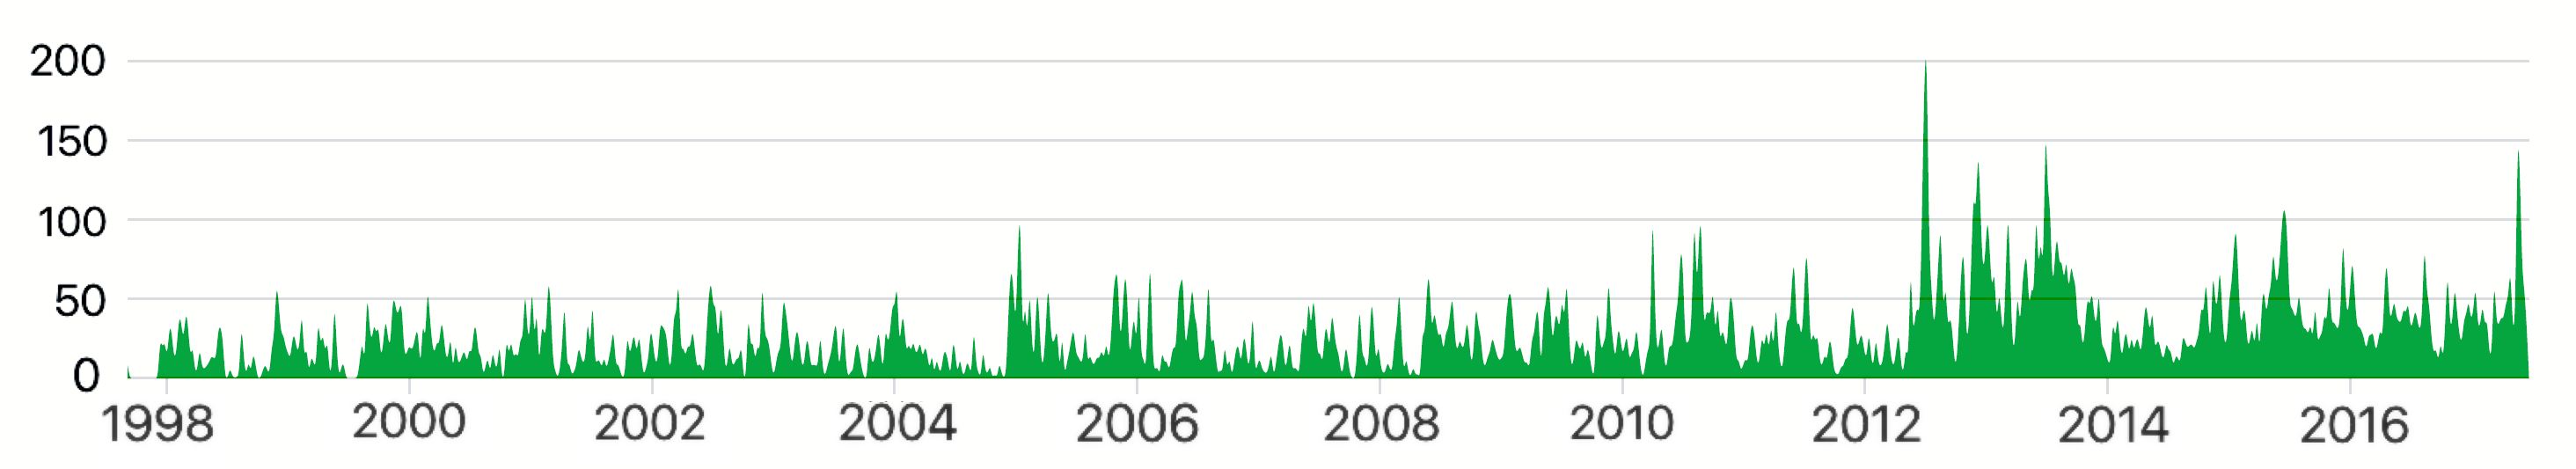
\includegraphics[width=\linewidth]{figs/commits.png}
\caption{This project will use data from many open source scientific programming projects, including the twenty year history available from tools like the deal.II finite elements library. Source: https://github.com/dealii/dealii/graphs/contributors}
\label{fig:commits}
\end{figure}


% \begin{table}[htbp!]
\footnotesize
\centering
\begin{tabular}{|p{\linewidth}|}
\hline
\bi
  \item \textbf{Formal method tools}  such as the SPIN~\cite{Ho11} model checker deploy automatic tools that are guided  quantified formulae which can succinctly express the correct, or incorrect, behavior of a large class of error;
  
  \item \textbf{Static code analyzers} such as Findbugs~\cite{Ay10} scan code looking for issues that might cause defective behavior such as possible logic errors that could lead to null pointer dereferences, bad casts, infinite recursive loops and other problems.  These tools suffer from large false positive reports. 
  
  \item Visser~\cite{Vis14} celebrates recent triumphs in optimizing SAT solvers and their applications to SE quality assurance.  Visser  also warns that automatic tools like SAT solvers are ``blackbox'' and software engineers need to look under the hood to make use of some of the internal results. Further, much work remains in order to fine-tuning such general tools to the specifics of any particular problem.

  \item Researchers in software analytics apply data mining algorithms to  build defect predictors using product attributes~\cite{Ha12} or process attributes~\cite{Ra13} extracted from software code. Foyzur et al. report that the data mining approach can be just as other methods such as effective static code analyzers~\cite{Fa13}.

\ei \\[-0.2cm]
Much prior work has explored the relative cost/benefits of using one or more of the above. For example,   Lowry warns that model checkers have severe scalability problems~\cite{Lo98}.  Also,~\cite{Ow07} comments that   conjunctions of these methods may find more bugs that any single one, but it is hard to predict before hand which, if any, of these methods finds most bugs.  Foyzur et al.~\cite{Fa13} notes that these, these defect prediction methods have fewer bindings to specific languages. This means that (e.g.) when a new version of C\# is realized, vendors of static code analyzers must scramble to adapt their tool to the nuances of the new language. Meanwhile, users of defect predictors can quickly build (in just a few hours) the lightweight parsers required to extract features from the new language.  \\ \hline
\end{tabular}
\caption{\textbf{Automatic methods for addressing code quality.} Since our goal is to monitor thousands of projects implemented in, potentially, dozens of languages, and since Foyzur et al. report that this method is as effective as more complex ones,  this research will take the data mining approach.}
\label{tab:methods}
\end{table}


% The second limitation with the tools of tools Table 1 is that they utilize automatic algorithms rather than  exploiting human domain knowledge.  In this age of the Internet, of social media, of everyone wired and on-line and sharing their ideas all the time, surely we  can augment (perhaps replace) automatic tools with more human expertise.  Previously, it was hard to collect all that human opinion, then assess which parts of that knowledge were useful/useless to some context. However, that is no longer the case. One side effect of more developers working on more open source projects is that many developers now routinely use a similar toolchain; e.g.  Jenkins for testing; Github for code storage/sharing; Jira for  issue tracking; Travis CI for continuous integration, and several other tools as well. \\

% This is a significant point since, once we build feature extractors from Github, Jenkins, Jira, Travis CI, etc, we extract  the  product, process, and resource data discussed above.. For example, since we have access to the source code of these systems (in Github) is it not difficult to extract code metrics. We can also automatically extract  resource and process information such as how often releases are made; how many active developers are part of each team; how long before developers move to different teams; what  developers touch what parts of the code; the time taken to close issues;  etc. Also, we can access quality measures such as reported bug rates, the achieved rate of enhancement within these systems, how many tests fail, how many old issues are re-opened, etc. Working in collaboration with our industrial partners at IBM Raleigh, over several months, we were able to gather data on 1646+ software projects of which 1108 were the most trending opensource projects on github and 538 were proprietary in-house projects. Upon mining these projects, we processed all the projects by running a ``sanity check''. We follow the guidelines of Kalliamvakou et al.~\cite{Ka14} to implement these ``sanity-checks'' which are then used to filter out all the projects.

% \begin{wraptable}[13]{r!}{0.6\textwidth}
\footnotesize
\centering
\caption{Sanity checks. Starting with 1108+538  open source+in-house projects, we discard  projects that {\em fail}
any of the LHS tests to arrive at 661+171 projects.}\label{tab:sanity}
\begin{tabular}{|l|r|r|}
\hline
Sanity check & \multicolumn{2}{c|}{\#discarded projects}                     \\ \cline{2-3} 
\multicolumn{1}{|c|}{(discard projects that violate these tests) }                              & \multicolumn{1}{l|}{In-house} & \multicolumn{1}{l|}{Open-source} \\ \hline
\# Pulls \textgreater 0                             & 35                            & 54                              \\
\# Issues \textgreater 10                            & 60                            & 89                              \\
\# Commits \textgreater 20                          & 68                            & 96                              \\
\# Developers \textgreater 8                        & 47                            & 67                              \\
\# Releases \textgreater 0                          & 136                           & 44                              \\
Project time frame \textgreater 1 year              & 12                            & 46                              \\
Projects doing only software development            & 9                             & 51                              \\ \hline
%Total Projects                                      & 538                           & 1108                            \\
Surviving projects                                  & 171                           & 661                             \\ \hline
\end{tabular}
\end{wraptable}


% \bi
% \item From the scientific programming arena, we can access detailed information about complex software. For example, see~\fig{commits} for 20 years of history about the deal.II finite elements software package. There are many other such scientific software projects that store their project data, on-line and readily available, in a similar manner\footnote{Dozens of such projects were presented at the recent 2017 PI meeting of the nsf  Software Infrastructure for Sustained Innovation (SI\textsuperscript{2}) https://github.com/si2-pi-community.github.io/2017-meeting/}. 

 

% \item Further, from the open source, we can explore a further 1108 open source projects.~\fig{projects} shows  details on some of the most widely known projects. We perform a sanity check to filter out projects that do not have sufficient data to perform the necessary analytics. Out of the 1108 projects, 661 passed our sanity checks (see~\tab{sanity}). 
% \ei

% % But a more important question is how to use all this data to achieve the goals of this research? I.e. how to use all this information to collect, summarize, audit and operationalize the expertise of seasoned software developers?  We can see three approaches. To answer, these questions, we must turn to cognitive psychology and some decades-old results from the field of knowledge acquisition. That material is discussed in the next section. In summary, we cannot just ask developers what process, product, and resource attribute ranges lead to high/low quality software being delivered late or on-time. Rather, we will propose a knowledge acquisition environment that extracts small fragments of knowledge about specific projects, then tests the generality of this fragments.
 
% % There are many similar examples in SE of how this theory explains certain expert incompetencies.  Many empirical results in SE suggest that sometimes expert developer behavior is actually hindered by their long-term memory.  The following studies all report problems where software developers hung on to patterns, without reviewing or revising them.  Another place where we must extend traditional STM/LTM theory is to explore cognition over long temporal periods. Much of the evidence for STM/LTM comes from the observations of short term incidents. 

% % \bi
% %     \item Ma et al.~\cite{Ma14} report that  STM contents are not long-lived and tend to be replaced every few seconds.    
% %     \item Griesche et al.  and Grigs et al.  study how brains cells change  while writing LTM ~\cite{Gr14} and how well human STM/LTM handles the user interface on autonomous cars~\cite{Gri13}.  The humans in those studies learned tasks for less than an hour (and in the case of~\cite{Gr14}, for less than than five minutes). 
% % \ei


% % \paragraph{\textbf{ISSUE \#2: What anti-patterns to apply?}}
% % \begin{wraptable}[13]{R}{0.56\linewidth}
\centering
\begin{tabular}{|l|l|l|l|l|l|}
\hline
 &\begin{turn}{90}Fowler'99~~\end{turn} & \begin{turn}{90}Lanza'06~~\end{turn} & \begin{turn}{90}SonarQube~~\end{turn} & \begin{turn}{90}Yamashita~~\end{turn} & \begin{turn}{90}Krishna'16~~\end{turn} \\ \hline
Fowler'99~\cite{Fo99}\cite{Ky05} & \cellcolor[HTML]{333333}{\color[HTML]{FFFFFF} 27} & 8 & 8 & 8 & 9 \\ \hline
Lanza'06~\cite{La06} &  & \cellcolor[HTML]{333333}{\color[HTML]{FFFFFF} 8} & 4 & 4 & 3 \\ \hline
SonarQube~\cite{Sq15} &  &  & \cellcolor[HTML]{333333}{\color[HTML]{FFFFFF} 8} & 5 & 5 \\ \hline
Yamashita'13~\cite{Ya13} &  &  &  & \cellcolor[HTML]{333333}{\color[HTML]{FFFFFF} 8} & 5 \\ \hline
Krishna'16~\cite{Kr16} &  &  &  &  & \cellcolor[HTML]{333333}{\color[HTML]{FFFFFF} 9} \\ \hline
\end{tabular}
\caption{Size of overlap  in what bad smells are endorsed/ supported by different tools or studies, from~\cite{Kr16}.}
\label{tab:smells}
\end{wraptable}
% % Table 1 shows a literature review~\cite{Kr16} on that topic: on the 27 anti-patterns proposed by Fowler~\cite{Fo99}, only very few are endorsed by other authors or supported by tools. This means that just because one developer strongly believes in the importance of a bad smell, it does not mean that belief transfers to other developers or projects. Developers can be clever, but their thinking can also be distorted by cognitive biases. Hence, as shown in \tab{smells}, developers, text books, and tools can disagree on which bad smells are important. Special tools are needed to assess their beliefs, for example, their beliefs in bad smells. Krishna et al.~\cite{Kr16}, show that tools like CrossTREE are one such candidate technology that can be used to assess the importance of bad-smells. They show that it is possible to use historical logs of software projects to identify which code-smells have been addressed in the past by developers. Then, using the information on if addressing these code-smells has had a positive impact in that past, we may recommend changes to future anti-patterns.

% % An interesting finding of that study is that different anti-patterns have different impacts on software quality. It is therefore difficult to know which anti-pattern needs to be fixed for specific projects without data mining tools like CrossTREE.

% % \paragraph{\textbf{ISSUE \#3: Can  anti-patterns be used for actionable and useful  change within a project?}}

% % In the summer of 2017, CrossTREE was deployed with at IBM in their BlueMix software suite. Bluemix is a cloud platform developed by IBM. It is an integrated DevOps tool that can be used to build, run, deploy, and manage applications on the cloud. Bluemix supports several programming languages including Java, Node.js, Go, PHP, Swift, Python, Ruby Sinatra, Ruby on Rails and it can be easily extended to support other languages (such as Scala).


% % Now, whenever BlueMix failed, it was for cognitive reasons like (a) recommendations were made at the wrong level; or (b) Recommendations do not take into account organizational factors etc. Given that we now have access to a large number of projects, we can actively monitor the evolution of these projects. This is shown in~\fig{venn}. Here \circled{A} represents the space of all possible artifacts that exist in a project. \circled{B} represents the artifacts that can be fixed of which developers may be willing to fix \circled{C}. There is a subset of the artifacts \circled{D} that have been changed historically. And \circled{E} represents the artifacts that anti-patterns recommend fixing. With IBM, we can monitor the 1646+ projects over long stretches of development to track these artifacts and recommend the right set of changes.



% % \paragraph{\textbf{RELATED WORK:}}   
% % Much of the current work in software analytics is on prediction not planning. CrossTREE is a planner. We distinguish planning from prediction for software quality as follows: 
% % Quality prediction points to the likelihood of defects. Predictors take the form:
% % \begin{equation*}
% %     out = f(in)    
% % \end{equation*}
% % where {\em in} contains many independent features (such as OO metrics) and {\em out} contains some measure of
% % how many defects are present. For software analytics, the function $f$ is learned via data mining (for static code attributes for instance).

% % On the other hand, quality planning generates a concrete set of actions that can be taken (as precautionary measures) to significantly reduce the likelihood of defects occurring in the future.

% % For a formal definition of plans, consider a defective test example $Z$, planners
% % proposes a plan $D$ to adjust attribute $Z_j$ as follows:

% % \begin{equation*}
% % \forall \delta_j \in \Delta :  Z_j =  
% % \begin{cases}
% %      Z_j + \delta_j& \text{if $Z_j$ is numeric}\bigstrut[t]\\
% %     \delta_j              & \text{otherwise}
% % \end{cases}
% % \end{equation*}

% % With this planner, to (say) simplify a large bug-prone method, our planners
% % might suggest to a developer to reduce its size (i.e. refactor that
% % code by, say, splitting it across two simpler functions).

% % %%%% END OF DOC %%%%%
% % % \begin{wrapfigure}[15]{R}{0.5\textwidth}
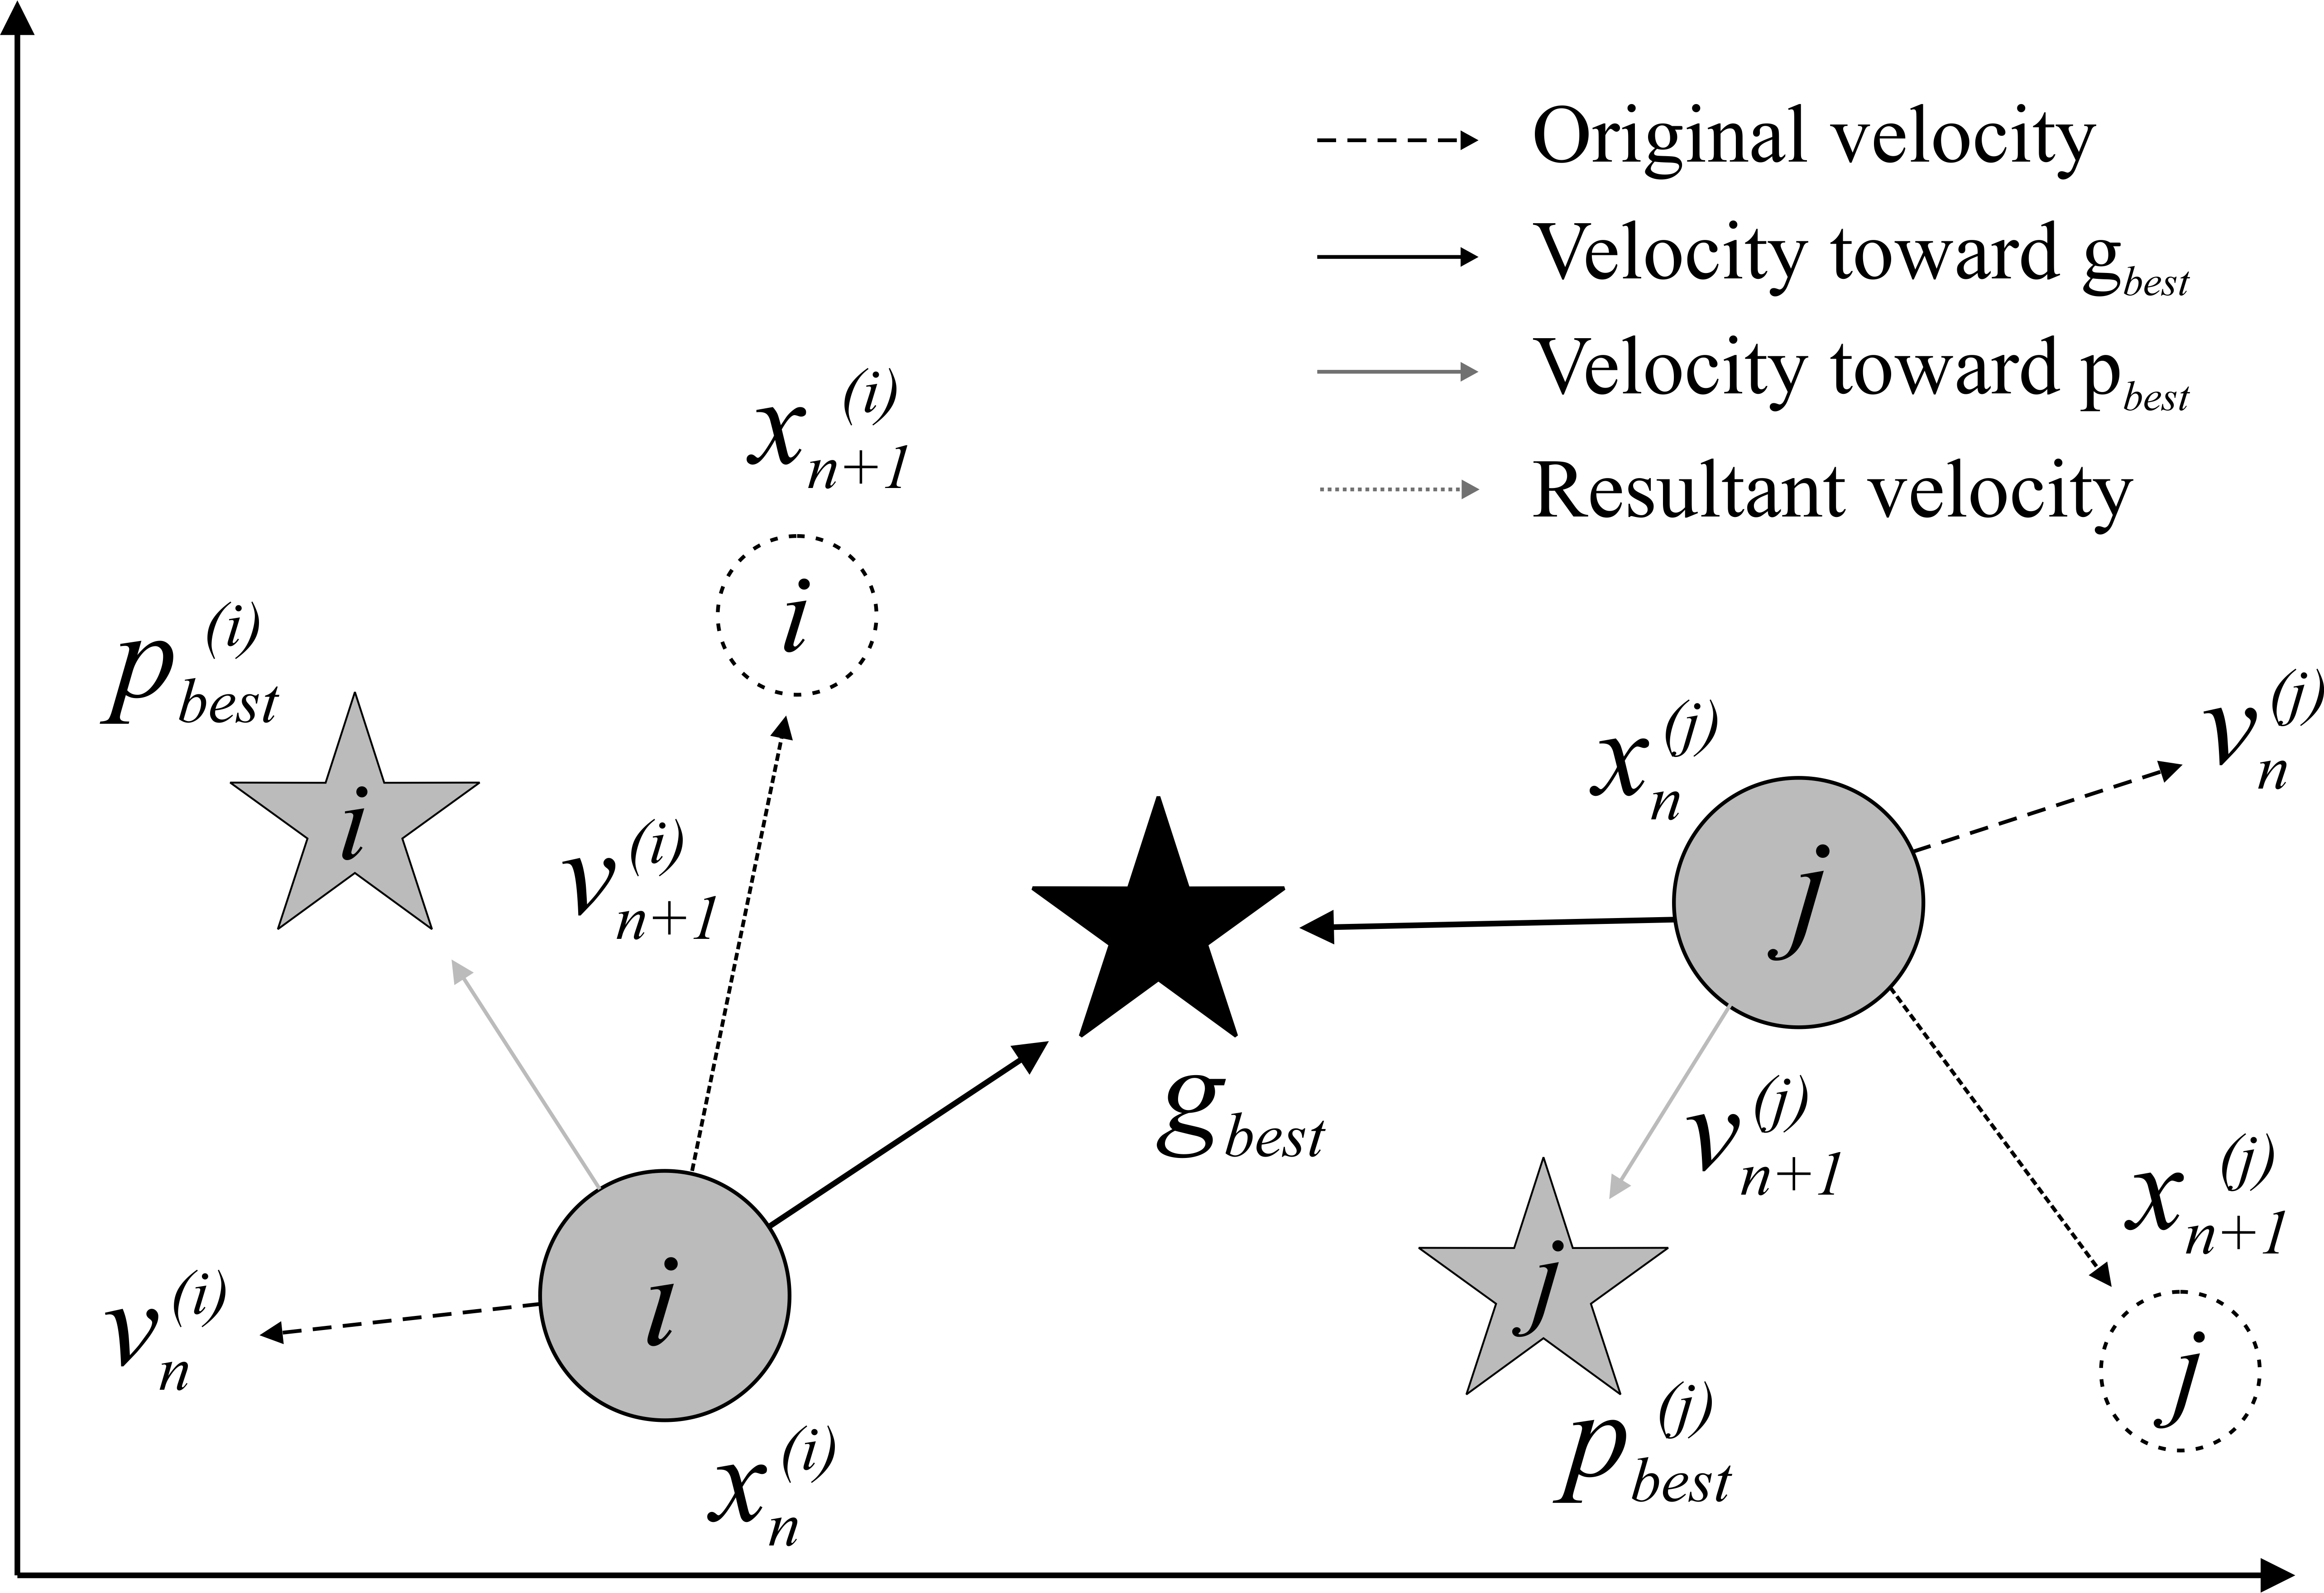
\includegraphics[width=\linewidth]{figs/pso_demo.png}
\caption{Mutations in PSO.}
\label{fig:pso}
\end{wrapfigure}


%%%%%%%%%%%%%%%%%%%%%%%%%%%%%%%%
\head{8. BROADER IMPACT AND EDUCATION:}
\paragraph{8.1. Benefits to Society at Large}
This proposal focuses on issues of
tremendous economic importance -- the creation of better quality software.
As a result, this work will increase America's ability for industrial and academic innovators to conduct
more scientific studies via computational means.  
 

\paragraph{8.2. Integration of Teaching and Research}
Much of the research in this project will also be integrated into a
classroom environment.  The PI teaches senior-level and graduate-level
SE, and software analytics   classes (and in those data mining
classes, all the case studies come from software engineering). All of
the technology developed in this proposal will become study
material for those subjects.  Replication studies are especially ripe
for classroom projects.  Also, through our publications and conference
work, we would publicize these tools as widely as possible with the
intent of supporting a broader community working with this approach.

\paragraph{8.3 Participation of Underrepresented
  Groups} The PI will continue their established tradition of
graduating research students for historically under-represented
groups.  PI Menzies' last two Ph.D. students were an African-American
women and a gentleman from an economically disadvantaged region
in central Pennsylvania.  Also, each summer, the PI's department runs an NSF-funded REU
 (research experience for undergraduates)
on the ``Science of Software''.
 At this
program, places are reserved for students from traditionally
under-represented areas (e.g. economically challenged regions of the
state of North Carolina) and/or students from universities
lacking advanced research  facilities.
Some of the simpler data mining concepts for this proposal would be suitable for lectures and REU projects.



%\input{f/under}
\paragraph{8.4. Dissemination of Knowledge}
 The PI has an extensive history of publishing at senior SE venues and so, it should be expected
that the results of this work will be widely visible.

Also, as mentioned above, the PI has a long history of publishing papers along with reproduction packages holding the data and the scripts required to
replicated the papers' results. All the our methods used here will be based around software tools in widespread   use (Github, Travis CI, etc).  We will release all our tools via open source licenses so our results can be readily applicable to researcher or developers using   Github, etc.
Although some of the data used in this study comes from private in-house projects,
the majority of our data comes open-source projects which we share with the community.

One issue here will be that it might be  too expensive
to let other groups download our  ingested data:
\bi
\item While we can certainly store our raw data on  S3,  Amazon   charges 4 cents per gigabyte download. Assuming our 5TB of data is downloaded 20 times a month for 3 years, that would cost \newline (\$0.05*1024*5*20)*36=\$184,320 $\approx$ 37\% of the grant (i.e. too much).
\item On the other hand, it is possible that our ingested data will occupy only a small fraction of the raw data-- in which case we can give free access
to our data to all
research groups.
\ei
Regardless of the above two points, we can certainly share all our scripts and bad smell detectors. These would allow other groups to replicated our results
after they conducted their own downloads.
 
 For more on this point, see our Data Management Plan.

 


\head{9. PRIOR RESULTS:}
This proposal is the next logical step in the PI's work on analytics.
{PI Menzies} has worked extensively in that arena.
In
\emph{``Automatic
Quality Assessment: Exploiting Knowledge of the Business Case''} (CCF-0810879, \$350,000, 08/08-06/11),
{PI Menzies} (with Bojan Cukic, WVU) built   generated many papers~\cite{jiang08a,me09n,me09i,me09b,me10d}
as well as one that is  was the third most-cited
paper in period 2009 to 2014 in the Journal of Empirical Software
Engineering.

In ``Better Comprehension of Software Engineering Data'' (CCF-1017330, \$500,000, 08/10-08/14).
{PI Menzies} (with Andrian Marcus, Wayne State),
explored various learning strategies (kernel estimation
methods, active learning tools, privatization methods) to
support defect and effort estimation. That work generated many papers~\cite{Bavota2010,Bavota2012a,Bavota2013,Bavota2012b,Haiduc2010a, Haiduc2013a, Haiduc2012a, Haiduc2013b, Marcus2010b, Ohlemacher2011b, Scanniello2013, Scanniello2011,me11m, peters12,Me13,me13a,peters12a}.
In terms \emph{broader impact}, that work graduated four masters and four Ph.D. students
and
spawned a small but active ``local learning'' research sub-community in SE (PI Menzies showed that
such ``local learners'' find better models
by first inferring local contexts, then building one model per context~\cite{Me13,me11m}).

  PI Menzies recently concluded
``Transfer Learning in Software Engineering'' (CCF-1302216, \$1,100,000, 08/13-07/18)
where {PI Menzies} (with Lucas Layman from Franhoufer Institute) 
building a toolkit to explore  methods for moving knowledge
learned from one software project to another.  That work  has generated
papers at TSE'18~\cite{krishna2018bellwethers}, ICSE'15~\cite{PetersML15}, ASE'15~\cite{krishna16}  and ESEM'13~\cite{he13} as well as the EMSE journal~\cite{Me17}, two IST journal papers~\cite{fu2016tuning,krishna2017learning},
one TSE paper~\cite{nam2017heterogeneous}.   A surprising and very useful outcome of that work
was the discovery of ``bellwethers'',  a simple transfer learner.

 PI Menzies has been working on  ``Scalable Holistic Autotuning for Software Analytics''
(CCF-1703487, \$898,349, 7/1/17-6/30/21) which is work with Co-PI Xipeng Shen
on using compiler technology to optimize very slow software analytics workflows. 
That work has several journal papers currently under review.

Also, since May'18 PI Menzies has worked on 
 EAGER: Empirical Software Engineering for Computational Science (CCF-1826574, \$124,628.00) looking at methods for applying empirical SE to computational science.
 That time has been spent interviewing domain experts and collecting data from
 Comp.Sci. projects.


\newpage
\head{Facilities, Equipment, and Other Resources:}
%\documentclass[10pt]{article}
%\usepackage{graphicx}
%\usepackage{subfigure}
%\usepackage{times}
%\usepackage{cite}
%\usepackage{subfigure}
%\usepackage{amsmath}
%\usepackage{amssymb}
%\usepackage{mscp}
%\usepackage{url}

%\begin{document}

\pagestyle{empty}
\setcounter{page}{1}
\setcounter{section}{0}
\setcounter{page}{1}
\setcounter{section}{0}

% \head{Facilities, Equipment, and Other Resources:}
NCSU completed the Engineering Building II on its Centennial Campus in
January 2006. The new building now houses the Computer Science
Department with its laboratories, which are accessible to the proposed
project. In particular, one laboratory will be devoted to the research
tasks of this proposal.

\paragraph{Facilities within NCS CS Department:}
The department has a 108-node compute cluster named ARC with about
2,000 cores (AMD Mangy-Cores), Infiniband QDR interconnect, per node
power monitoring, GPUs and SSDs and parallel file system support,
which was funded by an NSF CRI that he is the main PI of together with
5 co-PIs. 
%
The ARC facility is providing local and remote researchers with
administrator/root privileges for Computer Science experiments at
medium scale. This allows any of the software layers, including the
operating system and Infiniband switch network routing tables, to be
modified for experimental purposes, e.g., to experiment with different
network topologies.  For large-scale demonstrations, remote 
facilities will be utilized (see below).

%This platform can be used for software development of integrated
%architectures. We plan to experiment on multiple Intel Core i7 x86
%CPU/GPU platforms, AMD APUs, and 2 NVIDIA Tegra TK1 development kits
%in our lab. We also we plan to acquire additional integrated platforms
%as part of this grant, including an Intel Xeon Phi (Knight's Landing).

% \paragraph{Remote Computing Resources:}
% The PI has access to the GPU cluster and Infiniband cluster at the
% Thomas Jefferson National Accelerator Facility of the U.S. Department
% of Energy. The GPU cluster includes 117 Intel Nahalem nodes, equipped
% with over 200 Tesla S1070 in total and connected with QDR or SDR
% Ininiband. The Infiniband cluster contains three sub-clusters. One
% contains 224 nodes, each equipped with dual quad-core 2.53 GHz
% Westmere CPUs, 24 GB memory, and QDR (40 Gb/s) Infiniband; one
% contains 320 nodes, each equipped with dual quad-core 2.4 GHz Nehalem
% CPUs, 24 GB memory, and QDR (40 Gb/s) Infiniband; another contains 392
% nodes, each quipped with dual quad-core 1.9 GHz Opteron CPUs, 8 GB
% memory, and DDR (20 Gb/s) Infiniband.

\paragraph{Computing Resources:}
%% RECHECK
The College of Engineering at North Carolina State University has built
a distributed computing environment named ``Eos'' for engineering education.
The Eos environment consists of more than 1,000 public and private
workstations and supports more than 12,000 users campus wide.
The success of Eos in the College of Engineering has spawned similar
projects in other colleges and in the campus computing center. Recently,
these projects have merged into a single distributed computing system
supporting more than 30,000 faculty, staff, and students. This computing
environment not only serves the academic computing needs of the campus,
but is also becoming the primary means of communication between the students
and the faculty. A large number of software packages are available on the
Eos system.

Additionally, NC State University provides a High-Performance Computing (HPC) facility as a part of the initiative to provide state of the art support for research and academic computing. HPC system (called henry2) provides NC State students and faculty with entry and medium level high-performance research and education computing facilities, consulting support and scientific workflow support. The HPC ecosystem consists of 1233 dual Xeon compute nodes in the henry2 cluster. Each node has two Xeon processors (mix of dual-, quad-, six-, eight-, ten-core, twelve-core) and 2 to 6 GigaBytes of memory per core. The total number of cores increases as more cores are purchased and now exceeds 10000. The nodes all have 64-bit processors. All HPC projects have capability to run jobs using up to 128 processor cores up to 48 hours and smaller jobs up to a week.

\paragraph{Office:}
The PI has an
office in the CS Department.  The Engineering Building II
has adequate space to house all research assistants
working on this project. All offices are wired for high-speed network
access.

\paragraph{Other Resources:}
The departments provide the space and basic networking services to
carry out the experiments, secretarial and administrative support as
well as general-purpose office equipment ({\em e.g.}, fax, photocopiers,
etc.).




\newpage
\bibliographystyle{unsrt}
\bibliography{references,refs-rahul}

\end{document}
